\documentclass{uscthesis}

%%%%%%%%%%%%%%%%%%%%%%%%%%%%%%%%%%%%%%%%%%
%%% Options include: [forbinding], which produces 
%%% an alternative title page and an appropriate
%%% binding margin,  [honors] for Honors College theses,
%%% and [durt] for undergraduate thesis submitted as part
%%% part of the distinction in mathematics program.
%%%%%%%%%%%%%%%%%%%%%%%%%%%%%%%%%%%%%%%%%%

%%%%%%%%%%%%%%%%%%%%%%%%%%%%%%%%%%%%%%%%%%
%%  LaTeX Preamble
%%%%%%%%%%%%%%%%%%%%%%%%%%%%%%%%%%%%%%%%%%

\usepackage{graphics}
\usepackage{graphicx}
\usepackage{epsfig}
\usepackage{times}
\usepackage{amsmath}
%\usepackage[tight,footnotesize]{subfigure}
%\usepackage[subfigure]{tocloft}
\usepackage{subfig}
\usepackage{url}
\usepackage{hyphenat}
\usepackage{pdfpages}
\usepackage{chngcntr}
\usepackage{caption}
\usepackage{pdfpages}
%\usepackage[showframe, pass]{geometry}
\usepackage{titlesec}
\usepackage{apptools}
\AtAppendix{\titleformat{\chapter}[block]{\normalfont\Large\scshape\centering}{\appendixname~\thechapter:}{0.333em}{}}



%%%%%%%%%%%%%%%%%%%%%%%%%%%%%%%%%%%%%%%%%%
%% You should include above
%% any LaTeX packages that you need.  Most packages should work 
%% with this documentclass.
%%%%%%%%%%%%%%%%%%%%%%%%%%%%%%%%%%%%%%%%%

\usepackage[style=uscnumeric]{biblatex}
\bibliography{refs}


%%%%%%%%%%%%%%%%%%%%%%%%%%%%%%%%%%%%%%%%
%% The lines above specify a BibTeX style which controls 
%% the appearance of the bibliography and how citations to
%% the bibliography within the text will work.  It is based on the biblatex.sty
%% package and provides a Chicago style, as preferred by the Graduate School.
%% There are other acceptable styles.  Indeed, different academic disciplines
%% have different styles.
%% 
%% The line  \bibliography{references} will cause LaTeX is search for a file
%% called references.bib.  This file could be named differently.  For example
%% \bibliography{henry} would provoke a search for henry.bib.  The
%% file reference.bib (or henry.bib) is one you will have to produce.  It is
%% a BibTeX database of references you use.
%% 
%% There are a number of alternate ways to address your bibliographic needs.
%% See the documentation uscthesisdoc.pdf  for a discussion of the different options.
%%
%%
%% 
%%In any case, this  is a good spot to ask LaTeX to load what it needs to handle
%% literature citations and to layout the bibliography. 
%%
%%%%%%%%%%%%%%%%%%%%%%%%%%%%%%%%%%%%%%%%%%


\newtheorem{thm}{Theorem}[chapter]
\newtheorem*{thmun}{Theorem}
\newtheorem{cor}[thm]{Corollary}
\newtheorem{lem}[thm]{Lemma}
\theoremstyle{definition}
\newtheorem{defn}[thm]{Definition}
\newtheorem{ex}[thm]{Example}
\theoremstyle{plain}

%%%%%%%%%%%%%%%%%%%%%%%%%%%%%%%%%%%%%%%%%%%%
%%  These are just a few sample lines. Put here any 
%%  commands of your own devising that you want to use.
%%  If these examples are no use to you, omit them.
%%%%%%%%%%%%%%%%%%%%%%%%%%%%%%%%%%%%%%%%%%%%%


%%%%%%%%%%%%%%%%%%%%%%%%%%%%%%%%%%%%%%%%%%%%%%%%%%%%%%
%%             The Front Matter
%%  The section below deals with the material that comes 
%%  before the actual content of the document: The title 
%%  page, abstract, acknowledgments,etc.
%%
%%  Some of it is required.
%%%%%%%%%%%%%%%%%%%%%%%%%%%%%%%%%%%%%%%%%%%%%%%%%%%%%%

\title{Underwater Cave Mapping and Reconstruction using Stereo Vision}

\author{Nicholas}{Weidner}     %% First Name then 
                                 %% Last Name

\degreedate{2017}                      %% The year of graduation

%\month{December}                 %% Only for the honors option
                                 %% where it is REQUIRED

\otherdegrees{
Bachelor of Science\\
University of South Carolina 2016\\ [\baselineskip] %% The \\ on this line is 
}                                %% ESSENTIAL!

\degreename{Master of Science}     %% The Graduate School provides 
                                 %% a list of official degrees.
\field{Computer Science}              %% Fields also provided by the 
                                 %% Graduate School.
\college{College of Engineering and Computing}  %%As listed by Grad School

\advisor {Dr.}{Ioannis Rekleitis}{Director of Thesis}  %%% Be sure the 
\readera{Dr.}{Marco Valtorta}{Reader}     %%% third field is 
\readerb{Dr.}{Jason O'Kane}{Reader}          %%% the one used in 
\readerc{Dr.}{Song Wang}{Reader} %%% your department.
               %%% Only use as many as
%%% If you have just two readers, for example, leave out \readerc and
%%% \readerd
%%%
%%% For Honors College theses use \reader{}{}   NO third field.
%%% The commands \otherdegrees, \degree, \field, \college, \readera, etc.
%%% are not used under the honors option.
%%%%%%%%%%%%%%%%%%%%%%%%%%%%%%%%%%%%%%%%%%%%%%%%%%%%%%%

\dean{Cheryl L. Addy}{Vice Provost and Dean of the Graduate School}   %% The Dean of the Graduate School
                   %% BE SURE TO CHECK THE NAME OF THE
                   %%PERSON CURRENTLY HOLDING THIS POSITION	
		   %% and the correct title.		             		
                     %% For Honors College theses use
                     %% \schcsigner{}{}.  For example,
                     %% \schcsigner{Dr.}{Davis Baird}

\copyrightpage       %% This is optional. It makes a 
                     %% copyright page that will appear 
                     %% immediately after the title page.

\abstract{abstract}  %% This calls the file herkimer.tex but 
                     %% but you might replace herkimer by 
                     %% anything you like, for example by 
                     %% abstract. Note, the Graduate School
                     %% REQUIRES that PhD dissertations have 
                     %% abstracts.
                     %%
                     %% For Honors College theses use
                     %% \honorsabstract{}

%\summary{precis}     %% This command calls  precis.tex
                     %% It is only available with the honors
                     %% option and it is REQUIRED for Honors
                     %% theses. 

\acknowledgments{thanks} %% This calls the file thanks.tex 
%% This is optional       %% where you have put your 
                          %%acknowledgments.

%\dedication{dedication}   %% Calls dedication.tex
%%% Also optional

%\preface{forward}    %% Calls forward.tex.  Optional.

%\makeLoT               %% Issue this command if your work has 
                       %% four or more tables.  A list of tables 
                       %% will be produced automatically.

\makeLoF               %% works the same way but for figures.

%%%%%%%%%%%%%%%%%%%%%%%%%%%%%%%%%%%%%%%%%%%%%%%%%%%%%%%%%%%%
%%  Finally, here is the meat.  The idea is to compose a 
%%  .tex file for each section of your thesis or dissertation.  
%%  Then use LaTeX's \include command to put them all together.  
%%  Doing it this way makes it easier to change the order of 
%%  exposition as your writing is in progress.  Also it
%%  makes it easy to print out just one section. The \include
%%  command always starts a new page. So every section would 
%%  start on a new page.  If you would like for sections just
%%  to continue, after the appropriate vertical space, on the
%%  current page, then use the \input command instead of the 
%%  \include command.
%%%%%%%%%%%%%%%%%%%%%%%%%%%%%%%%%%%%%%%%%%%%%%%%%%%%%%%%%%%%

\begin{document}

\addcontentsline{toc}{chapter}{Introduction}
\chapter*{Introduction}\label{ch:intro}

The importance of underwater cave mapping spans several fields. First, it is crucial in monitoring and tracking groundwater flows in karstic aquifers. According to Ford and Williams~\cite{Ford1994} 25\% of the world's population relays on karst water resources. Our work is motivated from the Woodville Karst Plain (WKP) which is a geomorphic region that extends from Central Leon County around the ``Big Bend'' of Florida~\cite{Lane2001}. Due to the significance of WKP, the Woodville Karst Plain Project (WKPP) has explored more than 34 miles of cave systems in Florida since 1987~\cite{WKPP}, proving the cave system to be the longest in USA~\cite{WKPP1}. This region is an important source of drinking water and is also a sensitive and vulnerable ecosystem. There is much to learn from studying the dynamics of the water flowing through these caves. Volumetric modeling of these caves will give researchers a better perspective about their size, structure, and connectivity. These models have even greater importance than simply enhancing the mapping. Understanding the volume of the conduits and how that volume increases and decreases over space is a critical component to characterizing the volume of flow through the conduit system. Current measurements are limited to point-flow velocities of the cave metering system and a cross-sectional volume at that particular point. My thesis work introduces a fist step towards robotic mapping of an underwater cave. The proposed approach results in 3\hyp D reconstructions which will give researchers the above described capabilities. Furthermore, volumetric models will be incredibly helpful for those involved with environmental and agricultural studies throughout the area, and once perfected this technology could help map other subterranean water systems, as well as any 3\hyp D environment that is difficult to map. The Woodville Karst Plain area is sensitive to seawater intrusions which threaten the agriculture and the availability of drinking water; for more details see the recent work by Zexuan et al.~\cite{ZexuanReports2016}. Second, detailed 3\hyp D representations of underwater caves will provide insights to the hydrogeological processes that formed the caves. Finally, because several cave systems contain historical records dating to the prehistoric times, producing accurate maps will be valuable to underwater archaeologists. 

\begin{figure}[ht]
	\begin{center}
		%\leavevmode
		\begin{tabular}{ccc}
			\hspace{-0.2em}\subfloat[]{\fbox{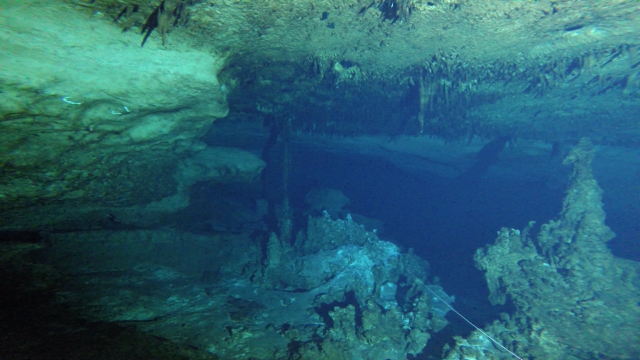
\includegraphics[width=.75\textwidth]{figures/Cave1S}\label{fig:beautyCave}}} \\
			\hspace{-0.5em}\subfloat[]{\fbox{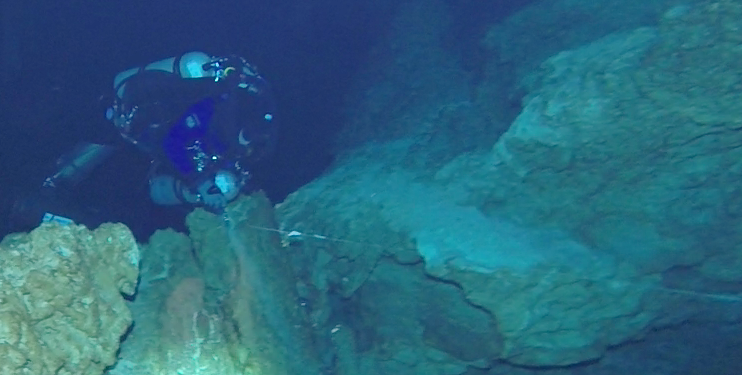
\includegraphics[width=.75\textwidth]{figures/DiverLine}\label{fig:diver}}}&
		\end{tabular}
	\end{center}
	\caption{\ref{fig:beautyCave} Typical Scene from an underwater cave. \ref{fig:diver} A cave diver attaching a branch line to the main line of a cave.}
	\label{fig:caveShots}
\end{figure}

Operations in underwater caves can be grouped under three categories: motion inside the known part of the cave; exploration of new territory; and surveying of newly explored areas. Most transportation in the explored part of caves is performed using diver propulsion vehicles (DPVs). All explored areas are marked by permanently attached cave line, which provides a direct route to the exit; see Fig. \ref{fig:diver} where a diver is inspecting the line. When divers explore uncharted territory, they proceed without the DPVs, laying out line and tying it to projections on the floor, walls, or ceiling. The third phase, surveying, consists of two divers measuring distances, using a cave\hyp line with knots every 3 m between attachment points. Simultaneously, the divers also measure the water depth at each attachment point, as well as the azimuth of the line leading to the next attachment point. All the information is recorded on a slate or waterproof paper. Estimates of the height and width of the passage can also be recorded, if time permits. The above described process is error\hyp prone and time consuming, and at greater depths results in significant decompression times, where total dive time can reach between 15 to 28 hours per dive. My thesis presents a first step of utilizing robotic technology to assist in cave exploration via the use of a stereo camera and a video\hyp light.  In many cases, during DPV rides, the divers attach cameras to their DPV and/or to themselves in order to document the exploration. Consequently, introducing a stereo camera does not complicate the standard operating procedures and will not increase the cognitive load of the divers.

The work of this thesis aims to achieve 3 goals.
\begin{enumerate}
	\item Study the implementation of camera calibration in a physical setting.
	\item Produce a point cloud of the underwater cave using stereo shape estimation and utilizing the presence of artificial light. 
	\item Reconstruct the surface of the cave out of the generated point cloud.
\end{enumerate} Combined, these pieces will come together to form a sufficient pipeline for reading image data and outputting a mapping of the cave system. This work can be easily adapted to a physical robot setting for later field use as described earlier. 

The next chapter will discuss a study of camera calibration along with effective methods for minimizing error in results. Chapter 3 covers the topic of scene reconstruction from stereo vision, and introduces a novel approach to generating point clouds of underwater cave systems\footnote{This chapter is joint work with Sharmin Rahman, Alberto Quattrini Li, and Ioannis Rekleitis and has appeared in the proceedings of the International Conference for Robotics and Automation (ICRA) 2017~\cite{weidner2017}.}. The last component, point cloud surface reconstruction, will be addressed in chapter 4. Finally, chapter 5 will conclude the work with a discussion of the overall contributions.    %% Calls Introduction.tex
                          %% Honors theses are required to 
                          %% have an Introduction.  For
                          %% Honors theses, the file 
                          %% Introduction.tex should begin
                          %%
                          %% \chapter*{Introduction}
                          %% followed by the text of the 
                          %% introduction.


\chapter{Camera Calibration}\label{chap:camcalib}
\section{Overview}\label{sec:caliboverview}
Camera calibration of the data acquisition cameras is a fundamental first step in achieving accurately scaled reconstructions. It is a highly studied and in common setups a solved problem. While much of the research of the community has passed the calibration phase, it is still the fundamental first step in a number of vision based research topics. Accurate calibration models and properly undistorted images are a necessity for any kind of accurate depth measurements, 3D reconstructions, or robotic navigation through a physical space via imaging. Good calibration relies on good input image data and sometimes this can be difficult to obtain. Cameras without digital screens make it impossible to view images or video until connected to a computer. This can make it difficult to validate the calibration set up while gathering input. In the underwater domain, cameras that lack this feature make data validation much more tedious and time consuming as the cameras must be removed from the water and connected to an external machine. If the data is being recorded in the field without additional equipment, it may be impossible to view the images or footage until data collection is complete. This can be even more problematic for stereo calibration systems where it is important that both cameras record the required information. As such, identifying the subset of collected data that results in the best calibration model is an important step in the calibration process.  

With such factors as affordability, durability, and quality becoming commonplace for the camera market, the use of cameras in research has grown. One popular brand is GoPro which develops small, durable, high resolution action cameras. GoPro cameras can be used in a number of domains including above and below water and on a number of different applications such as building reconstruction or ocean floor mapping. While the popularity of these cameras has increased, they are susceptible to some of the challenges in collecting good calibration data. Most GoPro models lack a screen for viewing images and footage during and after capture making it hard to position the camera in the scene. Part of this problem has been fixed with the introduction of new Bluetooth and smart phone features, but wireless communication is severely limited in the underwater domain. In the case of this work, there was a need to accurately undistort footage obtained using GoPro's SuperView capture mode. This mode causes severe distortion along the edge of the frame which some calibration tools have trouble overcoming. 

\begin{figure}[t]
	\centering
	\fbox{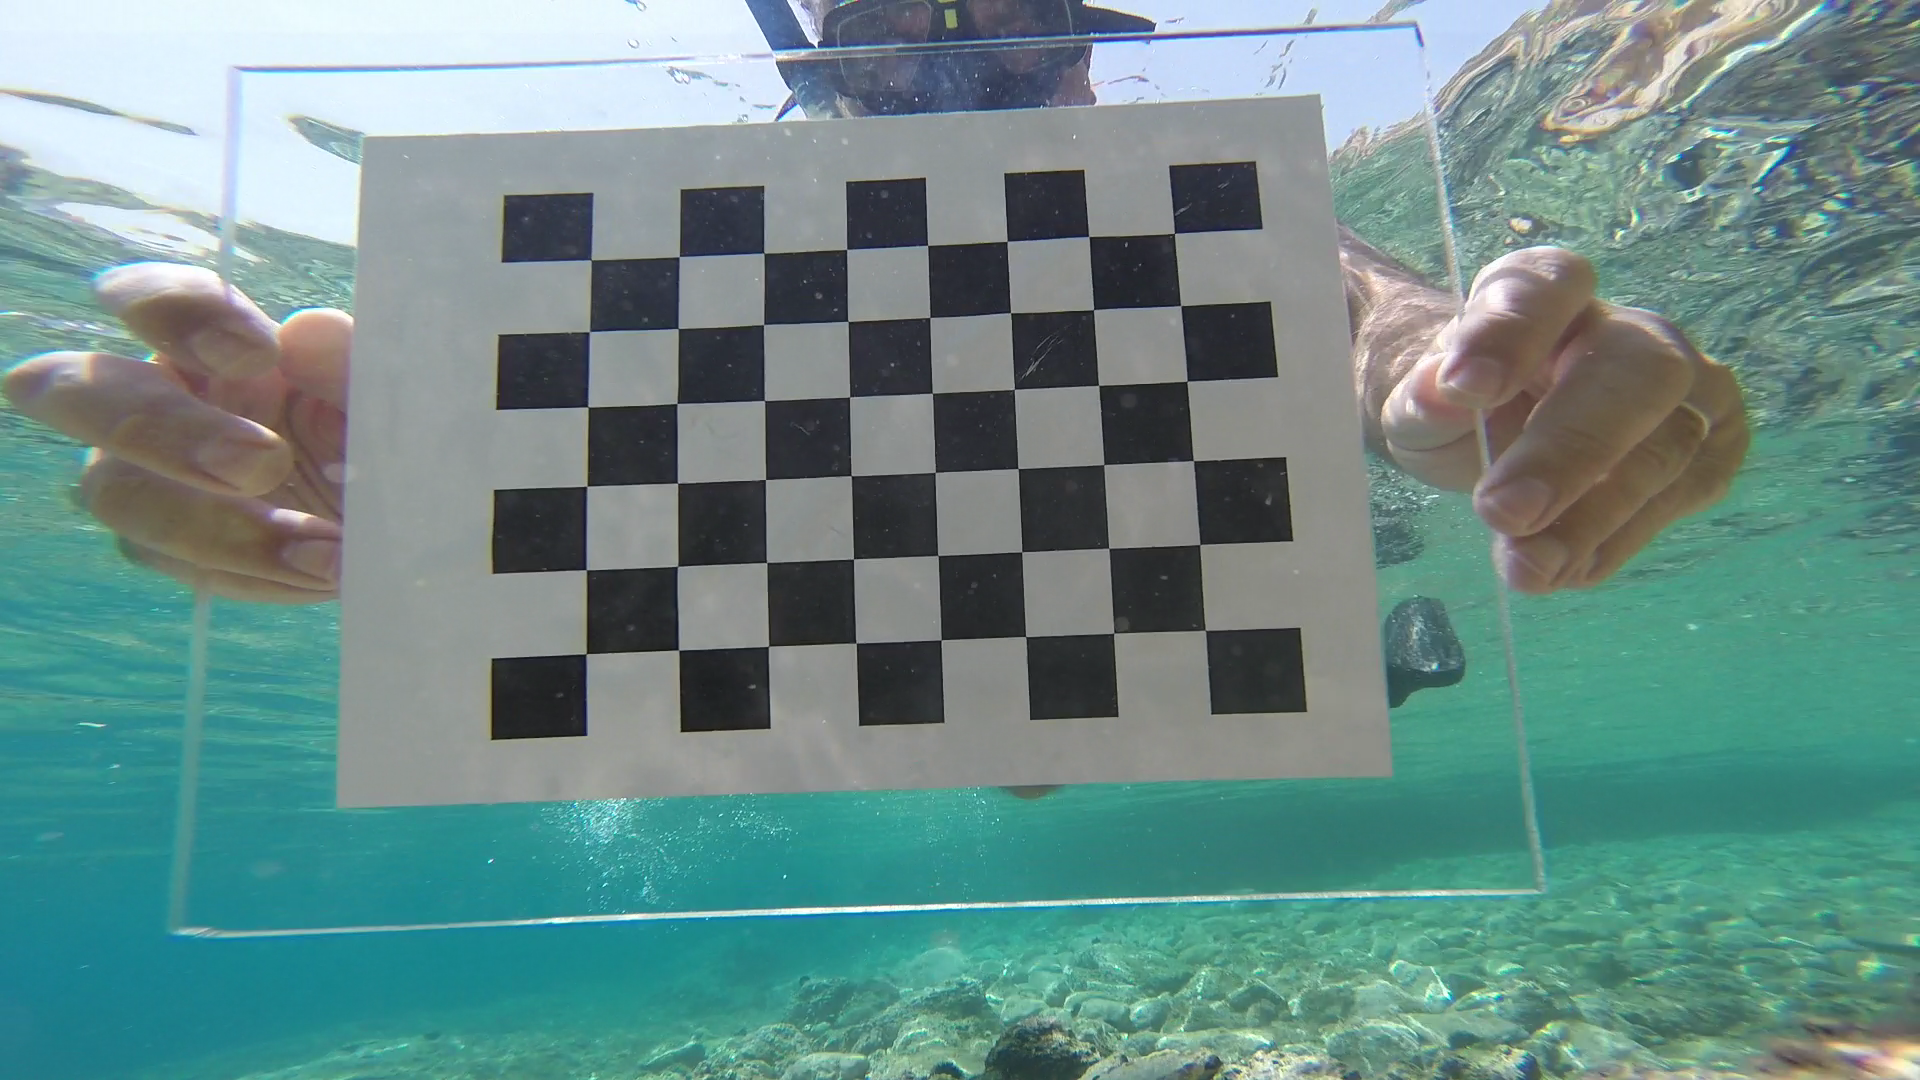
\includegraphics[width=0.75\textwidth]{./figures/right-0006.png}}
	\caption{An underwater image of a waterproof calibration checkerboard pattern used for camera calibration.}
	\label{fig:beauty}
\end{figure}

\section{Related Work}\label{sec:camrel}
Camera calibration is a well established method originating back to as early as the 1900s with lens research by Conrady~\cite{Conrady1919}. This developed into the Brown distortion model which forms the foundation for modern day camera calibration techniques~\cite{Brown1966,Brown1971,Brown1986}. One of the first openly available camera calibration tools was the Camera Calibration Toolbox for MATLAB. This tool, developed by Jean-Yves Bouguet, could calibrate a camera and return the intrinsic and extrinsic parameters. The toolbox was built on the foundation of work done by Tsai~\cite{Tsai1987} for introducing off the shelf technologies to camera calibration, Heikkila and Silven~\cite{Silven1997} for presenting an intrinsic calibration model, and most prominently Zhang for developing many of the techniques used in the toolbox~\cite{Zhang2000}. This work was later ported to OpenCV and used to develop the more powerful Computer Vision System Toolbox for MATLAB. These two tools are widely used in the field today. 

More complex calibration models have been developed to handle more complicated camera lenses taking into account different types of distortion. Specific methods to deal with extreme fisheye and barrel distortion have arose both in OpenCV and in independently released packages. Both the  Camera Calibration toolbox for MATLAB and OpenCV have a fisheye calibration model based on the work of Kannala and Brandt~\cite{Bradnt2006}. Scaramuzza have worked extensively with omnidirectional camera calibration and has developed his own MATLAB toolbox ~\cite{Scara2006_1,Scara2006_2,Scara2008_1,Scara2008_2}. Currently these are the state of the art readily available tools for rapid prototyping and used by the general public, each with its own advantages and disadvantages.

In recent years, there has been a push for the calibration of low cost and easily portable camera systems. With the development and continued advancement of products such as the GoPro, research has gone into the calibration and use of these cameras to solve imaging problems. Balletti et al. ~\cite{balletti2014calibration} explained many of the advantages of lightweight cameras including their ease to handle, capability of performing under extreme conditions, and providing high quality stills and video. They also explained methods for calibrating the cameras for reconstruction purposes. In the realm of underwater camera calibration, Schmidt and Rzhanov~\cite{schmidt2012measurement}, and Shortis~\cite{shortis2015calibration} compared the results and techniques for calibrating GoPro systems with the added distortion of water. These studies all fail to touch on the calibration of the GoPro camera when it is set to SuperView mode. 

\begin{figure}[t]
	\centering
	\fbox{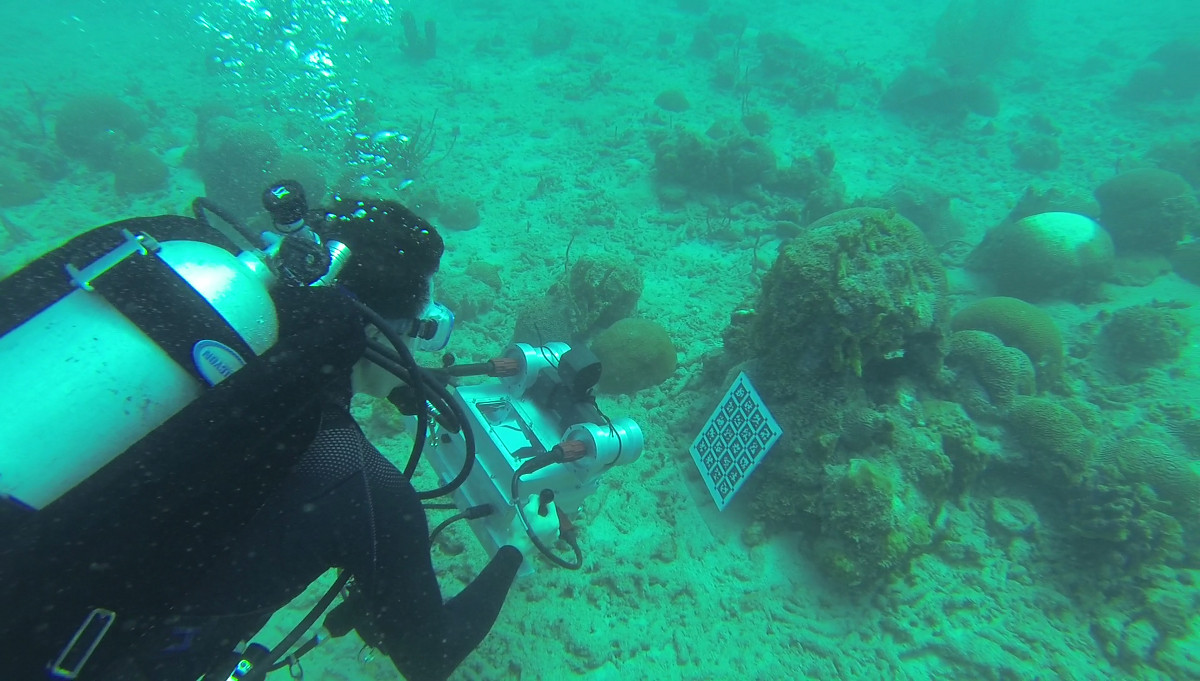
\includegraphics[width=0.9\textwidth]{figures/othersensors_red}}
	\caption{Diver calibrating an underwater rig consisting of stereo cameras and an IMU.}
	\label{fig:sensors}
\end{figure}

Calibration can be much more complicated and tedious if the camera is not the only sensor needing calibration. Many robotic systems take advantage of multiple proprioceptive and exteroceptive sensors in combination with visual input. A common proprioceptive sensor is the inertial measurement unit (IMU) which measures linear accelerations and angular velocities. Fig. \ref{fig:sensors} shows an example of the calibration process for a visual and interior sensor system. Significant efforts has been  in order to calibrate these systems as accurately as possible including the use of a Kalman Filter to determine the unknown coordinate transformations between sensors~\cite{4637877, doi:10.1177/0278364907079276, 2011_Kelly_Visual}. Because these calibrations rely heavily on the camera input, it is important that the camera calibration output is as accurate as possible so it will not skew the calibration of the other sensors. 



A system for assisting novice users to collect images for calibration through a Graphical User Interface is proposed by Richardson et al.~\cite{richardson2013iros}. 

Hu and Kantor~\cite{hu2016icra} presented a greedy approach for selecting images so that they are uniformly distributed over different camera poses. Such a method considers a budget that encodes the maximum processing time allowed. A quality metric could be considered to improve the performance.
%\section{Related Work}\label{sec:camrel}
Camera calibration is a well established method originating back to as early as the 1900s with lens research by Conrady~\cite{Conrady1919}. This developed into the Brown distortion model which forms the foundation for modern day camera calibration techniques~\cite{Brown1966,Brown1971,Brown1986}. One of the first openly available camera calibration tools was the Camera Calibration Toolbox for MATLAB. This tool, developed by Jean-Yves Bouguet, could calibrate a camera and return the intrinsic and extrinsic parameters. The toolbox was built on the foundation of work done by Tsai~\cite{Tsai1987} for introducing off the shelf technologies to camera calibration, Heikkila and Silven~\cite{Silven1997} for presenting an intrinsic calibration model, and most prominently Zhang for developing many of the techniques used in the toolbox~\cite{Zhang2000}. This work was later ported to OpenCV and used to develop the more powerful Computer Vision System Toolbox for MATLAB. These two tools are widely used in the field today. 

More complex calibration models have been developed to handle more complicated camera lenses taking into account different types of distortion. Specific methods to deal with extreme fisheye and barrel distortion have arose both in OpenCV and in independently released packages. Both the  Camera Calibration toolbox for MATLAB and OpenCV have a fisheye calibration model based on the work of Kannala and Brandt~\cite{Bradnt2006}. Scaramuzza have worked extensively with omnidirectional camera calibration and has developed his own MATLAB toolbox ~\cite{Scara2006_1,Scara2006_2,Scara2008_1,Scara2008_2}. Currently these are the state of the art readily available tools for rapid prototyping and used by the general public, each with its own advantages and disadvantages.

In recent years, there has been a push for the calibration of low cost and easily portable camera systems. With the development and continued advancement of products such as the GoPro, research has gone into the calibration and use of these cameras to solve imaging problems. Balletti et al. ~\cite{balletti2014calibration} explained many of the advantages of lightweight cameras including their ease to handle, capability of performing under extreme conditions, and providing high quality stills and video. They also explained methods for calibrating the cameras for reconstruction purposes. In the realm of underwater camera calibration, Schmidt and Rzhanov~\cite{schmidt2012measurement}, and Shortis~\cite{shortis2015calibration} compared the results and techniques for calibrating GoPro systems with the added distortion of water. These studies all fail to touch on the calibration of the GoPro camera when it is set to SuperView mode. 

\begin{figure}[t]
	\centering
	\fbox{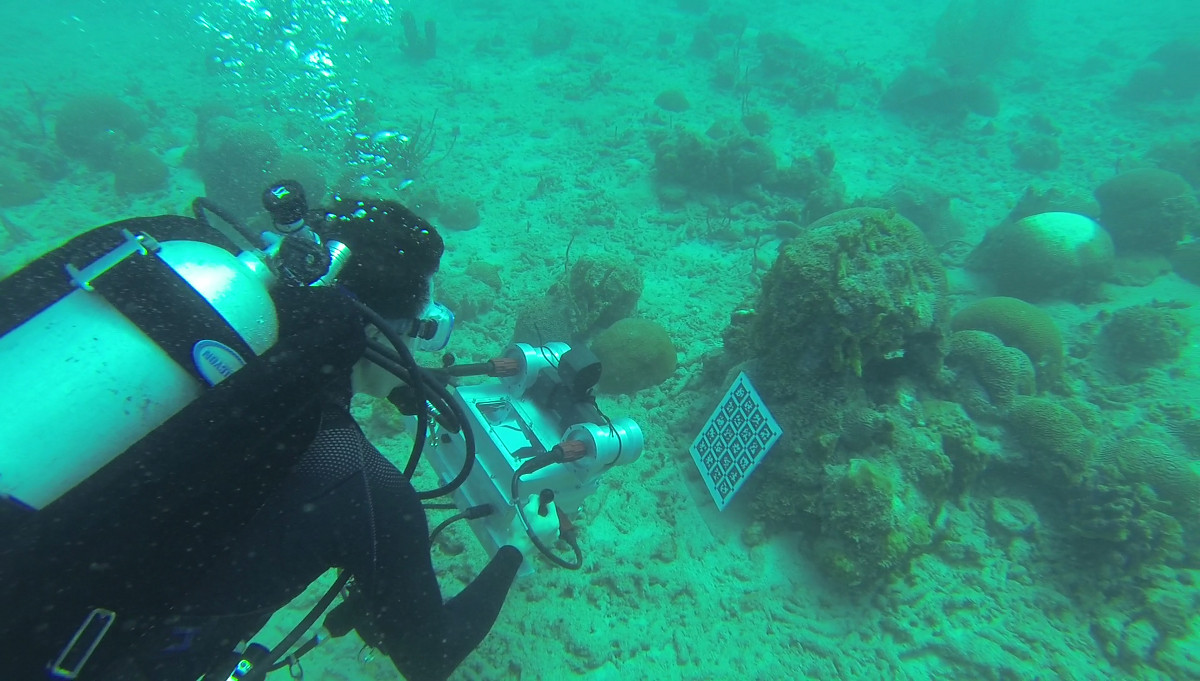
\includegraphics[width=0.9\textwidth]{figures/othersensors_red}}
	\caption{Diver calibrating an underwater rig consisting of stereo cameras and an IMU.}
	\label{fig:sensors}
\end{figure}

Calibration can be much more complicated and tedious if the camera is not the only sensor needing calibration. Many robotic systems take advantage of multiple proprioceptive and exteroceptive sensors in combination with visual input. A common proprioceptive sensor is the inertial measurement unit (IMU) which measures linear accelerations and angular velocities. Fig. \ref{fig:sensors} shows an example of the calibration process for a visual and interior sensor system. Significant efforts has been  in order to calibrate these systems as accurately as possible including the use of a Kalman Filter to determine the unknown coordinate transformations between sensors~\cite{4637877, doi:10.1177/0278364907079276, 2011_Kelly_Visual}. Because these calibrations rely heavily on the camera input, it is important that the camera calibration output is as accurate as possible so it will not skew the calibration of the other sensors. 



A system for assisting novice users to collect images for calibration through a Graphical User Interface is proposed by Richardson et al.~\cite{richardson2013iros}. 

Hu and Kantor~\cite{hu2016icra} presented a greedy approach for selecting images so that they are uniformly distributed over different camera poses. Such a method considers a budget that encodes the maximum processing time allowed. A quality metric could be considered to improve the performance.
\section{Theory}\label{sec:callibtheory}
The pin hole camera model is the simplest model for how a camera works and is used as the basis for modern implementations of camera calibration. With this model, intrinsic and extrinsic camera parameters define the transformation between 3D world coordinates and 2D image coordinates. The intrinsic parameters
disregard the position and orientation of the camera and define such parameters as the focal length, principal point, and aspect ratio. Extrinsic parameters define the pose between object frame and camera frame in terms of rotation and translation. The full model to get the pixel coordinates ($u$, $v$) of a point in the world $(X, Y, Z)$, including intrinsic and extrinsic parameters, is 
%
\begin{equation}
\lambda 
\left[\begin{array}{c} u \\ v \\ 1 \end{array} \right]
=
\begin{bmatrix}
f_x & 0 & c_x \\ 0 & f_y & c_y \\ 0 & 0 & 1
\end{bmatrix}
\begin{bmatrix}
r_{11} & r_{12} & r_{13} & t_1 \\ r_{21} & r_{22} & r_{23} & t_2 \\ r_{31} & r_{32} & r_{33} & t_3
\end{bmatrix}
\left[\begin{array}{c} X \\ Y \\ Z \\ 1 \end{array} \right]
\end{equation}
%
where $\lambda$ defines the scale, $u$ and $v$ describe the coordinates of the newly projected image pixel point, $f_{x}$ and $f_{y}$ describe the focal length values in pixels over width and height of the camera sensor, $c_{x}$ and $c_{y}$ describe the principal point coordinates in pixels, $r_{ij}$ represent the elements of the extrinsic rotation matrix, $t_i$ represent the elements of the extrinsic translation matrix, and $X$, $Y$, and $Z$ are the 3D coordinates in the world reference frame. The extrinsic matrix is what translates 3D coordinates $X$, $Y$, and $Z$ to new coordinates $X_{new}$, $Y_{new}$, and $Z_{new}$ in the camera reference frame. This transformation equates to
%
\begin{equation}
\left[\begin{array}{c} X_{new} \\ Y_{new} \\ Z_{new} \end{array} \right]
=
R
\left[\begin{array}{c} X \\ Y \\ Z \end{array} \right]
+ t
\end{equation}
%\[
%u=\dfrac{f_{x}*X}{Z}+c_{x}
%\]
%\[
%v=\dfrac{f_{y}*X}{Z}+c_{y}
%\]
%
Then, using triangle equivalence, assuming a unit distance between the Center of Projection where all the ray lights project in the camera and the image plane, the pixel $X_{new}'$ and $Y_{new}'$ in normalized image coordinates can be determined as follows, :
%
\begin{equation}
X_{new}'=X_{new}/Z_{new}
\end{equation}
\begin{equation}
Y_{new}'=Y_{new}/Z_{new}
\end{equation}
Taking into account the intrinsics parameters of the camera, we can then find the projected $u$ and $v$ pixel coordinates on the actual image plane: 
\begin{equation}
u=f_{x}*X_{new}'+c_{x} 
\end{equation}
\begin{equation}
v=f_{y}*Y_{new}'+c_{y}
\end{equation}

When actual cameras are examined, calibration must take into account the distortion resulting from the lens. Distortion is separated between radial and tangential distortion. Radial distortion is caused by the light bending near the edges of the lens. MATLAB defines the distortion along the $x$ (columns) and $y$ (rows) coordinates of the camera as: 
%
\begin{equation}
x_{r\textit{distortion}} = X_{new}'(1+k_{1}r^{2}+k_{2}r^{4}+k_{3}r^{6})
\end{equation}
\begin{equation}
y_{r\textit{distortion}} = Y_{new}'(1+k_{1}r^{2}+k_{2}r^{4}+k_{3}r^{6})
\end{equation}
%
where $k_{i}$ are the radial distortion coefficients and $r^{2} = X_{new}'^{2}+Y_{new}'^{2}$. Tangential distortion is the result of the lens unparallel to the camera sensor plane. MATLAB defines the $x$ and $y$ of this distortion as 
%
\begin{equation}
x_{t\textit{distortion}} = [2*p_{1}*X_{new}*Y_{new}+p_{2}*(r^{2}+2*X_{new}'^{2})]
\end{equation}
\begin{equation}
y_{t\textit{distortion}} = [p_{1}*(r^{2}+2*Y_{new}'^{2})+2*p_{2}*X_{new}'*Y_{new}']
\end{equation}
% 
where the $p_j$ are the tangential distortion coefficients and $r^{2} = X_{new}'^{2}+Y_{new}'^{2}$. 
%
These distortions can be introduced into the perspective projection as

\begin{equation}
u=f_{x}*X_{new}'*(x_{r\textit{distortion}}+x_{t\textit{distortion}})+c_{x}
\end{equation}
\begin{equation}
v=f_{y}*Y_{new}'*(y_{r\textit{distortion}}+y_{t\textit{distortion}})+c_{y}
\end{equation}
resulting in the pixel coordinates $u$ and $v$ in the image plane.
%\[
%or
%\]
% OpenCV also includes the implementation of a fish eye camera model for more extreme radial distortions. In this model a $\theta$ is introduced as $\theta=\arctan(r)$. This is then used to define a fisheye distortion of the scene as
% %
% \[
% \theta_{distortion}=\theta(1+k_{1}\theta^{2}+k_{2}\theta^{4}+\theta_{3}r^{6})
% \]
% These distortions can be introduced into the perspective projection as
% \[
% u=\dfrac{f_{x}*x*\theta_{\textit{distortion}}}{z*r}+c_{x}
% \]
% \[
% v=\dfrac{f_{y}*y*\theta_{\textit{distortion}}}{z}+c_{y}
% \]


Using known world coordinates and identifying how the camera transforms points in a 2D image, the intrinsic $[f_x,f_y,c_x,c_y]$ and extrinsic $[R|t]$ parameters can be calculated, where $R$ and $t$ are the matrix and vector that represents the rotation with elements $r_{ij}$ and the translation with elements $t_i$. Testing the accuracy of the resulting model is done by reprojecting the points backwards through the model and identifying how close the points lie to where they were originally. The average distance these points are off from where they should be is the reprojection error and is used to identify how good the model is. Reprojection error measures pixel units and ideal models should minimize reprojection error as much as possible.

Once the error is as an acceptable level---typically below 1 pixel---the images can be undistorted using the calibration parameters. Because the intrinsic parameters have nothing to do with the image scene, they can be used to undistort any collection of images taken with the same camera. If the domain changes, for example the camera is moved from above water to underwater, the distortion coefficients will no longer accurately represent the image distortion. Because of this, the camera needs to be calibrated for both underwater and on above water  undistortion. While theoretically the introduction of a water distortion model could eliminate the need for calibrating directly underwater, practically this was found unnecessary. 

While this describes the process of monocular camera calibration, in a stereo system there is also the step of rectification. Rectified images are undistorted images with an additional rotation applied in order to make the epipolar lines of the image parallel. They also use an altered projection matrix that shifts the images apart by a distance described by the baseline of the cameras. The baseline is the distance between the optical centers of each camera. In a horizontal stereo setting, matching epipolar lines in each camera would have identical $y$ coordinates. The new rectified projection matrices in a horizontal stereo system are
%
\begin{equation}
P1 =
\begin{bmatrix}
f_x & 0 & c_{x1} & 0\\ 0 & f_y & c_y & 0\\ 0 & 0 & 1 & 0
\end{bmatrix}
\end{equation}
\begin{equation}
P2 =
\begin{bmatrix}
f_x & 0 & c_{x2} & T_x * f_x\\ 0 & f_y & c_y & 0\\ 0 & 0 & 1 & 0
\end{bmatrix}
\end{equation}
%
where $T_x$ is the horizontal shift amount. The rectified $u'$ and $v'$ coordinates can again be defined as 
%
\begin{equation}
u'=P1*R*P1^{-1}*u
\end{equation}
\begin{equation}
v'=P2*R*P2^{-1}*v
\end{equation}
%
and the rotation matrix $R$ is defined so the epipolar lines along both images are now parallel. This is a vital step in any kind of reconstruction work, because it allows a matching algorithm to reduce the search space to find the distance between matching features in stereo image sets; the output can then be used for the triangulation of 3D world points using such a distance, also called disparity.
\section{Calibration Data Collection}\label{sec:calibdatacollection}
The common approach among calibration techniques is to use a set of points with known relationships, for example points in a grid pattern. The points are usually extracted from a set of input images as the corners, or centers of blobs. On these input images distinct features are needed so that it is possible to easily identify the spatial relationship of points in space compared to how the camera perceives them. Common approaches use calibration targets with black and white squares or circles with known dimensions. The checkerboard pattern is one of the standardized approaches, see Fig. \ref{fig:beauty}. The intersection of white and black squares creates distinct points in space, all the points exit on the same plane along parallel lines, and the square size provides accurate measures physical distance between the points. Thus, the undistorted (rectified) images can be checked if they preserve the linear relations between points. 

\begin{figure*}[th]
	\begin{center}
		%\leavevmode
		%\begin{tabular}{ccc}
		\fbox{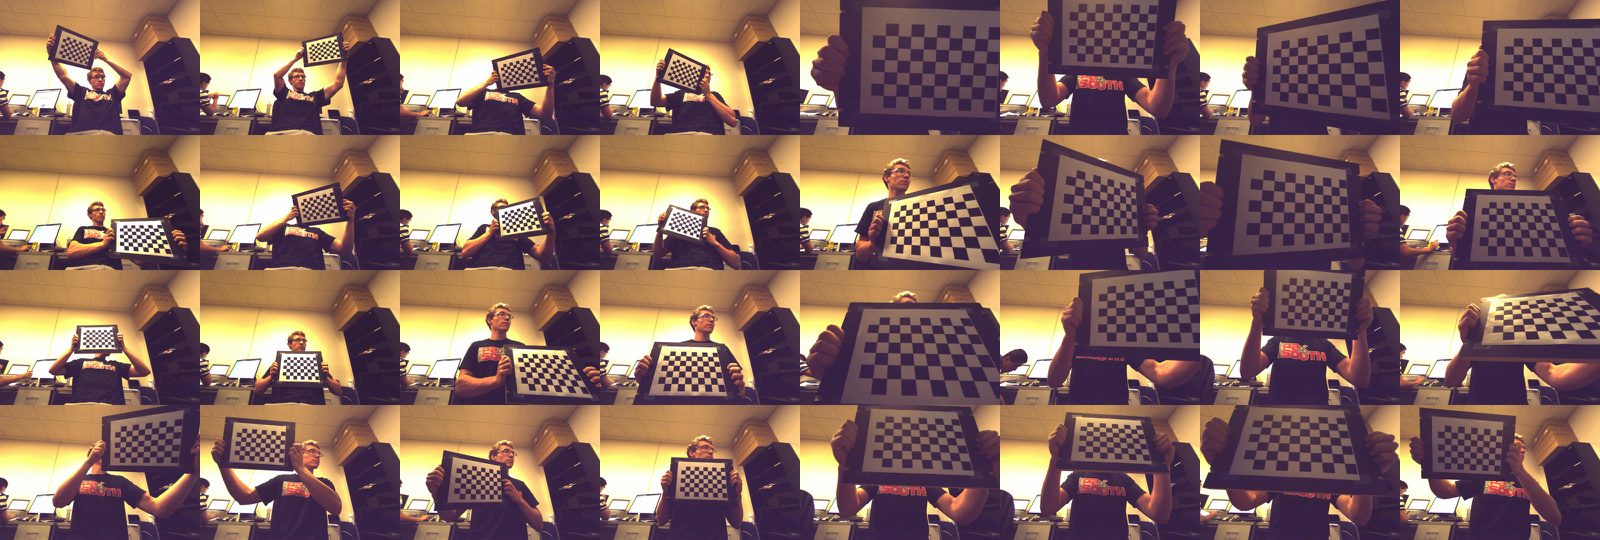
\includegraphics[width=.9\textwidth]{figures/combine_images_final.jpg}}
		%\end{tabular}
	\end{center}
	\caption{A collection of good viewing angles and distances for a calibration board}
	\label{fig:goodAngles}
\end{figure*}

When collecting images using a calibration target there are a number of important factors to consider. The input images should show the calibration board at a variety of locations, depths, and angles. Fig. \ref{fig:goodAngles} shows a collection of images taken when calibrating the stereo rig shown in Fig. \ref{fig:sensors}. The calibration was performed using the OpenCV fisheye camera calibration functions. This set of images highlights the important lessons learned. First there are views of the board from different distances, from far to near as seen left to right respectively. Second, 
the board is skewed with respect to the image plane; this is achieved by tilting the target to be non parallel to the camera. Third, the board should never be rotated past 90 degrees otherwise the images can be flipped; it is worth noting that using an odd by even dimension calibration pattern makes the board robust to orientation changes. The pattern should be visible in the field of view in its entirety, although this is an obvious point, when there are no preview capabilities it can be challenging. In particular, when calibrating a stereo system the pattern should be fully visible in both the left and the right camera.

\begin{figure*}[ht]
	\begin{center}
		\leavevmode
		\begin{tabular}{ccc}
			\subfloat[]{\fbox{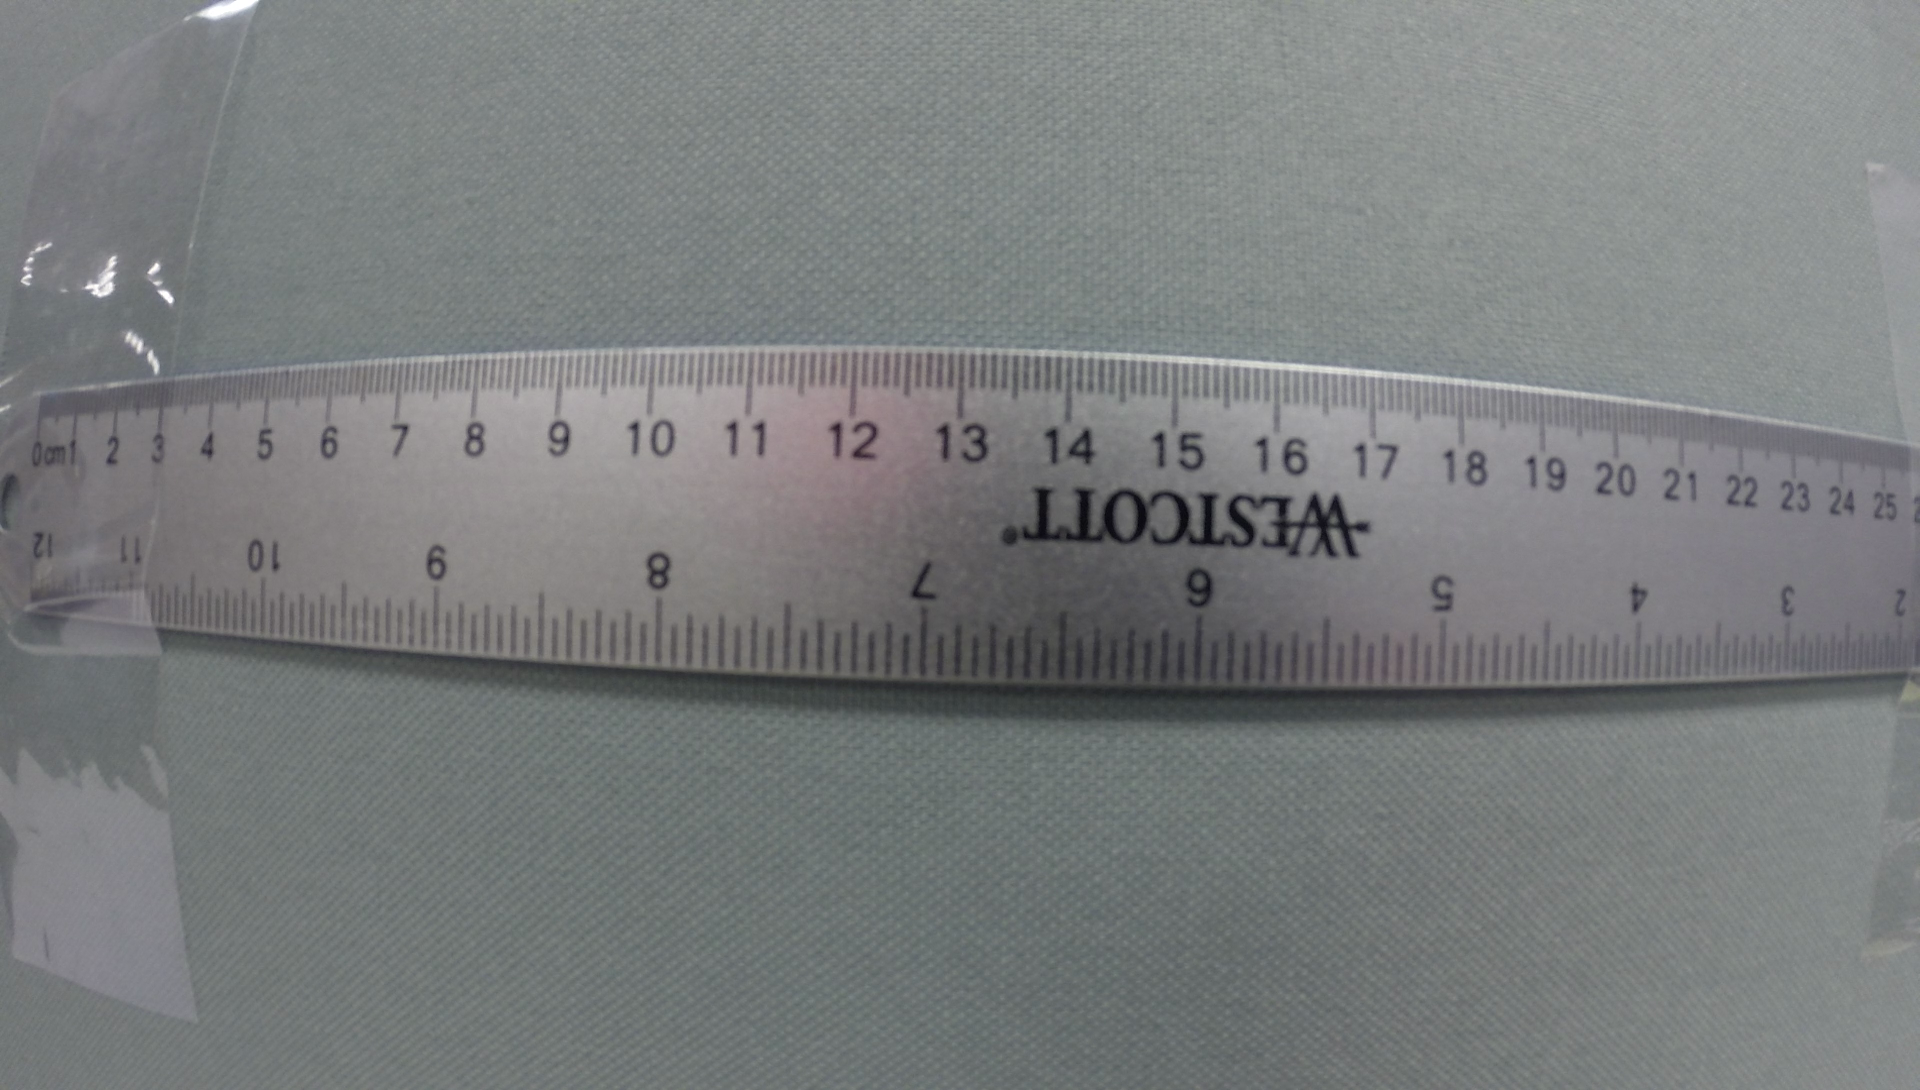
\includegraphics[width=.4\textwidth]{figures/without_superview.png}\label{fig:withouts}}} &
			\subfloat[]{\fbox{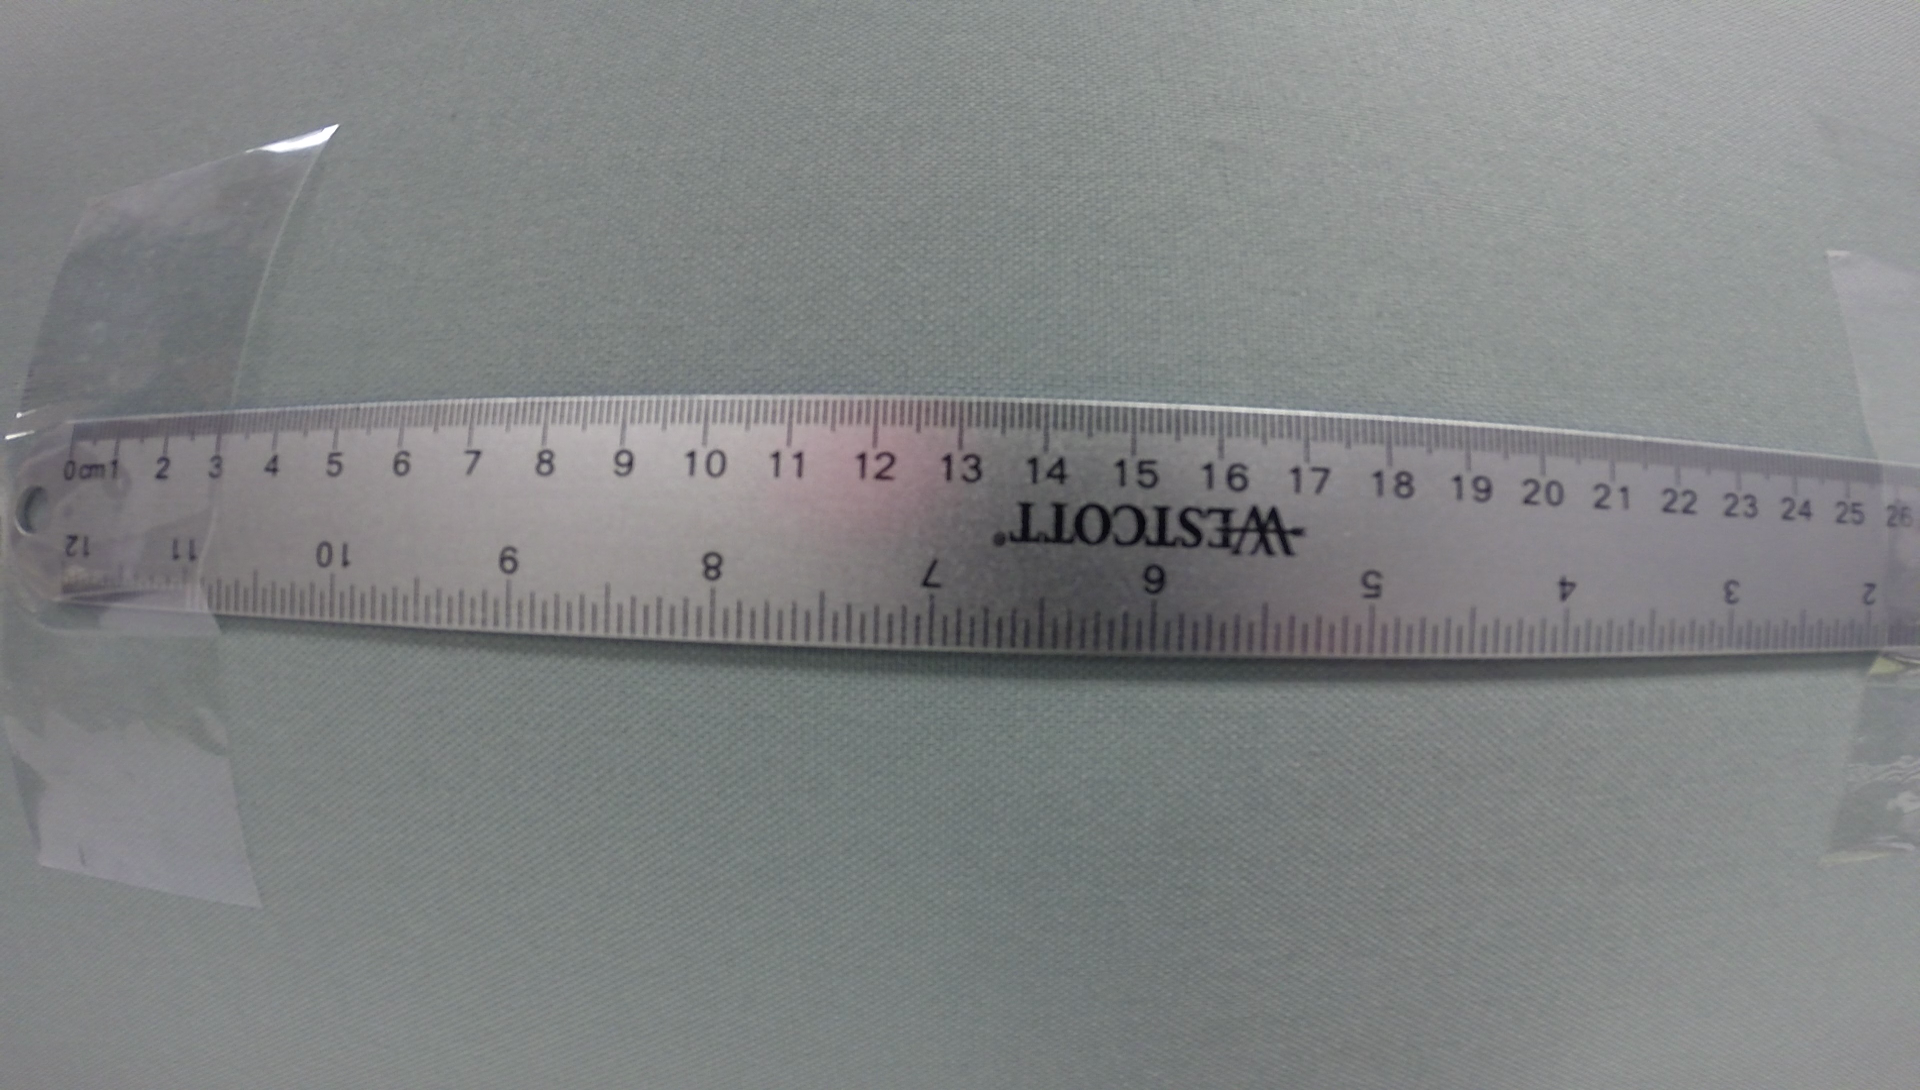
\includegraphics[width=.4\textwidth]{figures/with_superview.png}\label{fig:withs}}}&
		\end{tabular}
	\end{center}
	\caption{From the same camera pose, (a) 1080p GoPro footage without the SuperView feature. (b) 1080p GoPro footage with the SuperView feature.}
	\label{fig:comparisons}
\end{figure*}
\section{SuperView}\label{sec:superview}
The GoPro cameras starting with Hero 3+ are employing a video capture mode termed {\em SuperView}. According to GoPro, SuperView works by dynamically stretching the 4:3 aspect ratio of the original image into a 16:9 aspect ratio. This keeps the center of the frame unchanged, but severely distorts the edges. The outcome is an image that captures more of the standard 1080p resolution mode. The exact image transform GoPro uses to fit the new aspect ratio is undisclosed so removing the distortion in post processing is not an option. As can be seen in Fig. \ref{fig:comparisons}, there is a drastic difference in images collected in GoPro's SuperView mode and their scene vertically and adjusts the aspect ratio to fit a standard wide screen. Many standard video editing software packages such as Adobe Premier, Adobe After Effects, or GoPro's own GoPro Studio have undistortion features, but these apply a stylistic look which does not help to calibrate the camera properly. 
\section{Calibration with MATLAB}\label{sec:calibmatlab}
As mentioned earlier, there are two standard, widely used, packages for camera calibration, one in MATLAB and one in OpenCV; both based on the same theoretical formulation. 
The MATLAB Computer Vision system Toolbox calibration implementation includes a feature for visualizing the reprojection error across input images as a graph; see Fig. \ref{fig:results1}. This graph also plots a mean reprojection error line which can help to identify which input images caused the most problems with the calibration. There is also an adjustable threshold line to set a maximum acceptable reprojection error, resulting in removing outlier images with reprojection error above the set threshold. In other words, by setting this threshold level after calibration, the system can reject the images above the line and rerun the calibration on only those images below. If the input data set is large (several tens to hundred of images), this can help cut down the input images to a more manageable  number between twenty and fifty. Furthermore, when calibrating, there is an option to use two or three distortion coefficients. The GoPro cameras we experimented with, calibrate best using two coefficients, but cameras with severe radial distortion work better with three.

While adjusting such features as the number of coefficients or the reprojection error threshold can result in a better camera model, it is important to avoid false positive reprojection error results. Using too many distortion coefficients can minimize the reprojection error, but rectified images generated with those parameters can be dramatically distorted. It is also important when removing outliers to avoid fitting the model to a non diverse image set. When removing outliers, try to keep images from distinct calibration pattern positions with lowest reprojection error. Also viewing the rectified images and scene reconstructions can validate if the parameters were accurate or not. 
Careful examination of the outliers images captured in SuperView mode indicated that points detected near the boundary of the image were badly misplaced due to the extreme distortion. 

\begin{figure}[bh]
	\centering
	\fbox{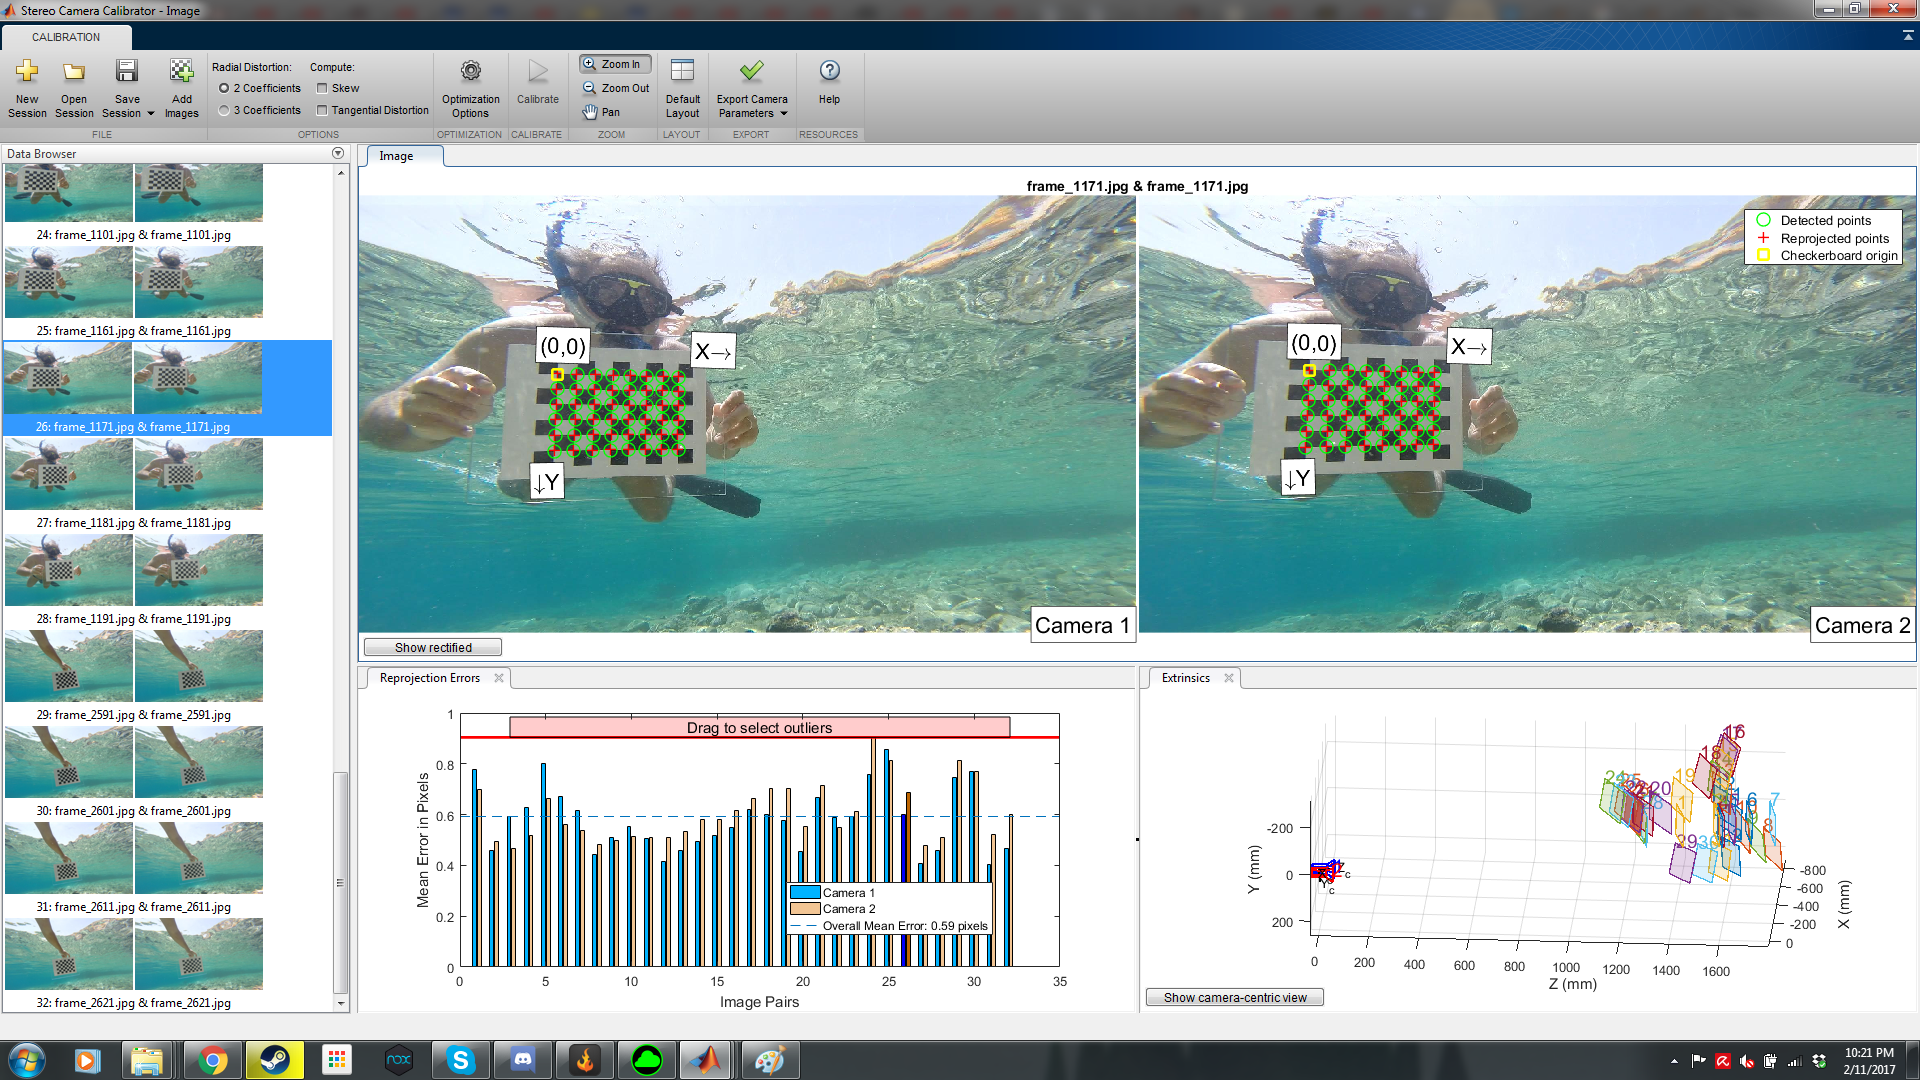
\includegraphics[width=0.95\columnwidth]{./figures/Results_01.png}}
	\caption{MATLAB Stereo Calibrator App GUI.}
	\label{fig:results1}
\end{figure}
\section{Experimental Results}\label{sec:calibmatsults}
\paragraph*{Experimental Setup}In our results we used a 8x6 calibration board with 25mm squares when underwater, and a 7x6 calibration board with 29mm squares when on air. We found the use of an odd by even size calibration board avoided the possible problem of upside down corner detection. In our underwater footage this did not interfere with our underwater results so our old set up still used. The board was printed on waterproof paper and glued onto an acrylic board as smoothly as possible to avoid any extra noise. 

\begin{figure*}[hp]
	\centering
	\subfloat[Non-filtered underwater dataset without SuperView]{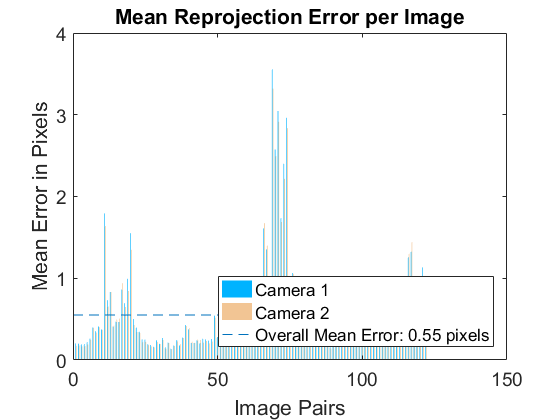
\includegraphics[width=.49\textwidth]{figures/no_sup_unw_before}}
	\subfloat[Filtered underwater dataset without SuperView]{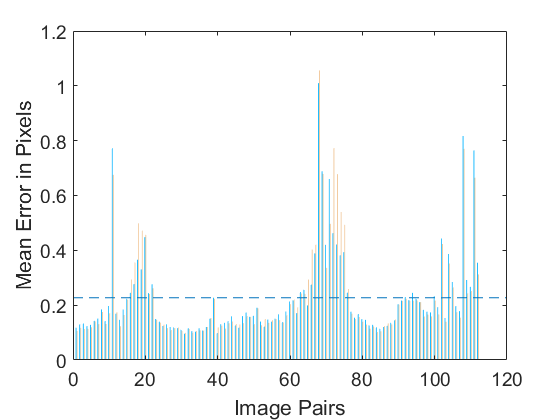
\includegraphics[width=.49\textwidth]{figures/no_sup_unw_after}}
	
	\subfloat[Non-filtered underwater dataset with SuperView]{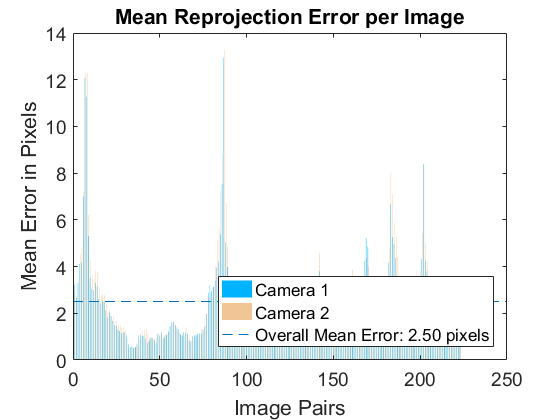
\includegraphics[width=.49\textwidth]{figures/with_sup_unw_before}}
	\subfloat[Filtered underwater dataset with SuperView]{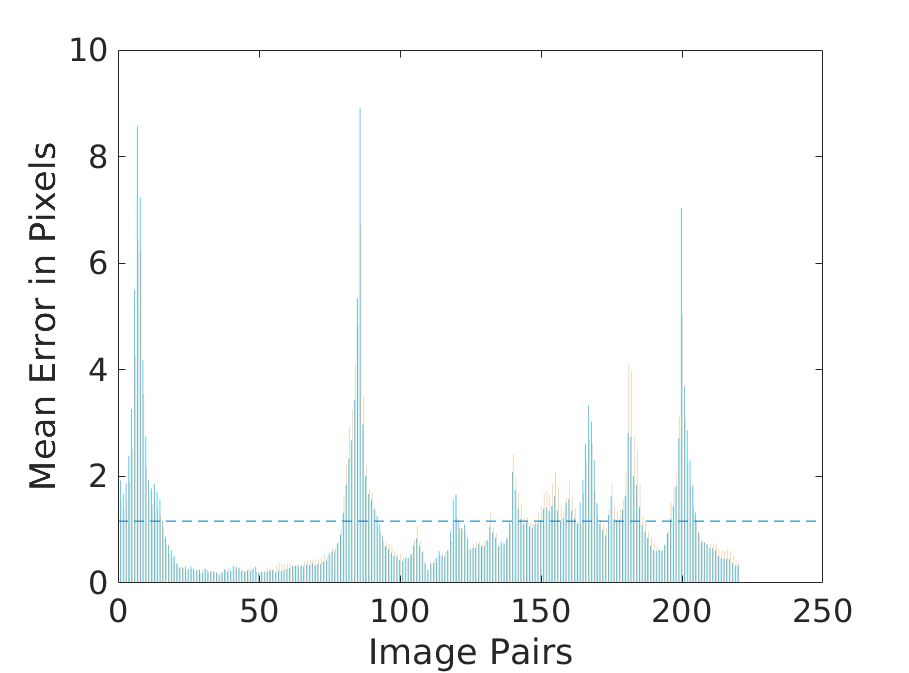
\includegraphics[width=.49\textwidth]{figures/with_sup_unw_after_fix}}
	\caption{Calibration results using MATLAB on underwater datasets. On the left column, results by using all the images, on the right column, results by filtering the dataset using the outlier removal method.\label{fig:MATresults}}
\end{figure*}

\begin{figure*}[hp]
	\centering
	\subfloat[Non-filtered above water dataset without SuperView]{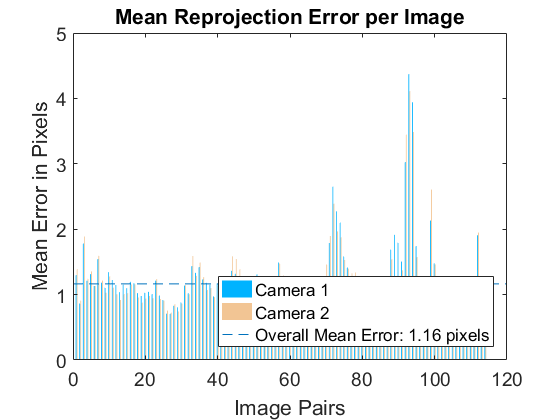
\includegraphics[width=.49\textwidth]{figures/no_sup_abvwat_before}}
	\subfloat[Filtered above water dataset without SuperView]{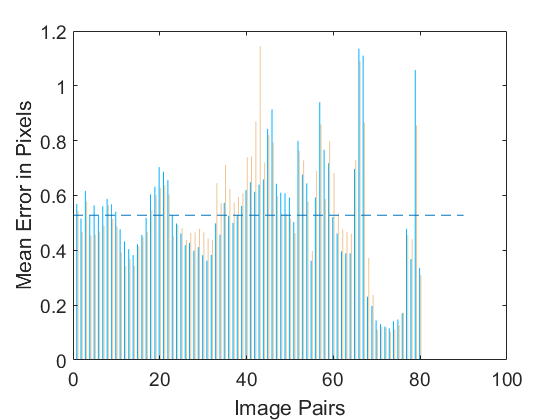
\includegraphics[width=.49\textwidth]{figures/no_sup_abvwat_after}}
	
	\subfloat[Non-filtered above water dataset with SuperView]{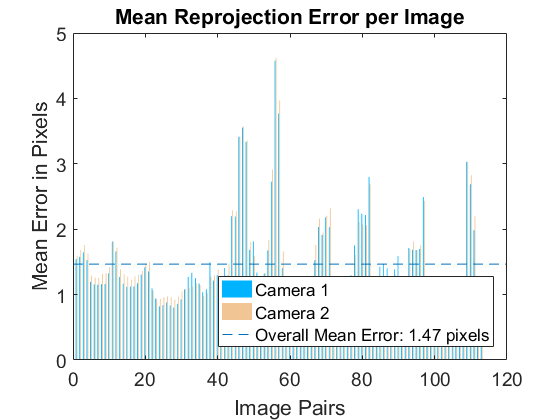
\includegraphics[width=.49\textwidth]{figures/with_sup_abvwat_before}}
	\subfloat[filtered above water dataset with SuperView]{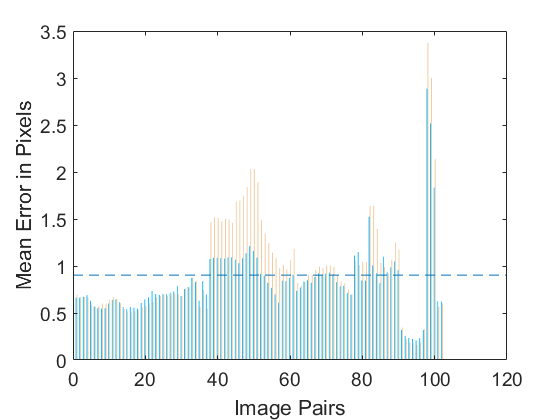
\includegraphics[width=.49\textwidth]{figures/with_sup_abvwat_after}}
	\caption{Calibration results using MATLAB on above water datasets. On the left column, results by using all the images, on the right column, results by filtering the dataset using the outlier removal method.\label{fig:MATresults2}}
\end{figure*}

\paragraph*{Calibration Procedure and Results}Using the left and right frames extracted from our calibration video, the images were run through the MATLAB Computer Vision system Toolbox Stereo Camera Calibrator upon which a result was determined. The reprojection error graph was examined in order to identify image pairs that exceeded the average image pair mean. These pairs were then removed from the input image list and the process was rerun. This happened repeatedly until either the total reprojection error fell within a specified reasonable range, or the image pair set became to small for meaningful calculations to be done. 

Using this method, we were able to calibrate a GoPro camera recording in SuperView mode with reprojection error of 0.9 on air and 0.51 underwater, compared to an error of 2.5 on air and 1.5 underwater without any outlier removal, as seen in Fig. \ref{fig:MATresults}.

Fig. \ref{fig:MATresults} compares the reprojection error results of image sets both with and without SuperView and both above and below water. 
In each case, calibration parameters were determined using a subset of full input data set---training phase---where the outliers had been removed. These parameters were then used to calculate the reprojection error of the full set once again---validation phase. 
Note that, in MATLAB, the function provided that recovers the extrinsics given the set of 2D-3D points of the checkerboard is based on a closed form formulation, while the one used inside the function for estimating the camera parameters is using a numerical optimization algorithm. As such, reprojection errors calculated on the same images from the training phase and the validation phase could be slightly different. In our experiments it was around 1-2 pixels. As such, we formulated the recovery of the extrinsics as a numerical optimization problem and we compute the error using a numerical optimization algorithm.
It can be observed that the mean pixel error is lower on the full set when the parameters from the image subset are used. Many plots still have outlier cases which result from a few possibilities. One cause is that while the corners were all detected by the corner detector, there was motion blur that skewed the actual location of the points. A second cause is the SuperView dynamic stretching that pulls the corner points outward near the edges. This effect is not completely eliminated after calibration which signifies features very close to the edge of the scene are not usable in any future processes. A future study might evaluate the region for which undistorted SuperView images remain undetected by the dynamic stretching. Comparing the results of image sets above and below water, underwater sets had a number of more sharp outlier cases. This is most likely the results of the difficulty in actually acquiring underwater calibration footage. The two domains did both had success in producing low reprojection error. In our case we even got slightly better error results from using SuperView underwater compared to above water, possibly because of the additional water distortion effect.
%%\section{OpenCV Port}
While the MATLAB Computer Vision system Toolbox is highly powerful and produced good results for our setup, there are drawbacks. Namely MATLAB is closed source software that requires payment to use. At the same time, MATLAB can be tedious to integrate with external applications and thus might not be ideal if camera calibration is only a part of a larger pipeline. OpenCV on the other hand is both widely used for a variety of image and computer visions applications, and is both open source and easy integrate. As noted earlier, OpenCV has implementations of camera calibration already and they are simple to use. Unfortunately they lack the user interface and built in outlier removal to make calibrating something like SuperView efficient. A similar implementation of the MATLAB outlier removal system was thus developed as an easy to use tool in OpenCV.

Because data visualization plays such a crucial role in identifying bad calibration input images, there needed to be a good way to generate interactive graphs of the OpenCV calibration results. This can be time consuming in C++, so alternatively python's Matplotlib library was used to recreate as similar output as possible to MATLAB's. OpenCV has both a C++ and a python library, but python was found to quite slow in calibrating large data sets. Due to this, a hybrid C++ and python application was created. The finalized control flow is as follows. 

\begin{enumerate}
	\item The C++ application reads in a set of input image pairs for calibration
	\item The calibration board corner points are detected and stored in an external file
	\item The first calibration run takes place and the reprojection error of every input image is stored in an external file along with the average reprojection error
	\item A python script reads the reprojection errors and plots them along with an average reprojection error line
	\item The user adjusts the average reprojection error line, selects outlier removal button, and the file of corner points is edited down to the new smaller set
	\item The C++ application reads in the corner points, avoiding time spent calculating the corner points again, and recalculates the reprojection errors with the new set
	\item The output is again used in the python script and the process is repeated
\end{enumerate}

Fig. \ref{fig:cvrepro} shows the plot generated by the OpenCV port, and the reprojection error for the image set of \ref{fig:results1}. After iterative outlier removals, the error is brought down from the original 2.83 to 1.02. This compares to MATLAB's error output of .51. Because MATLAB is a closed source application, the exact method for calibration can not be ported over directly. This means MATLAB's calibration probably involves a slightly refined calculation and optimization. OpenCV has trouble matching MATLAB's results and its speed, but compared, but this method still provides an open source alternative. These results match or are even better than hand picking input images and saves time eliminating bad options. 

\begin{figure}[th]
	\centering
	\fbox{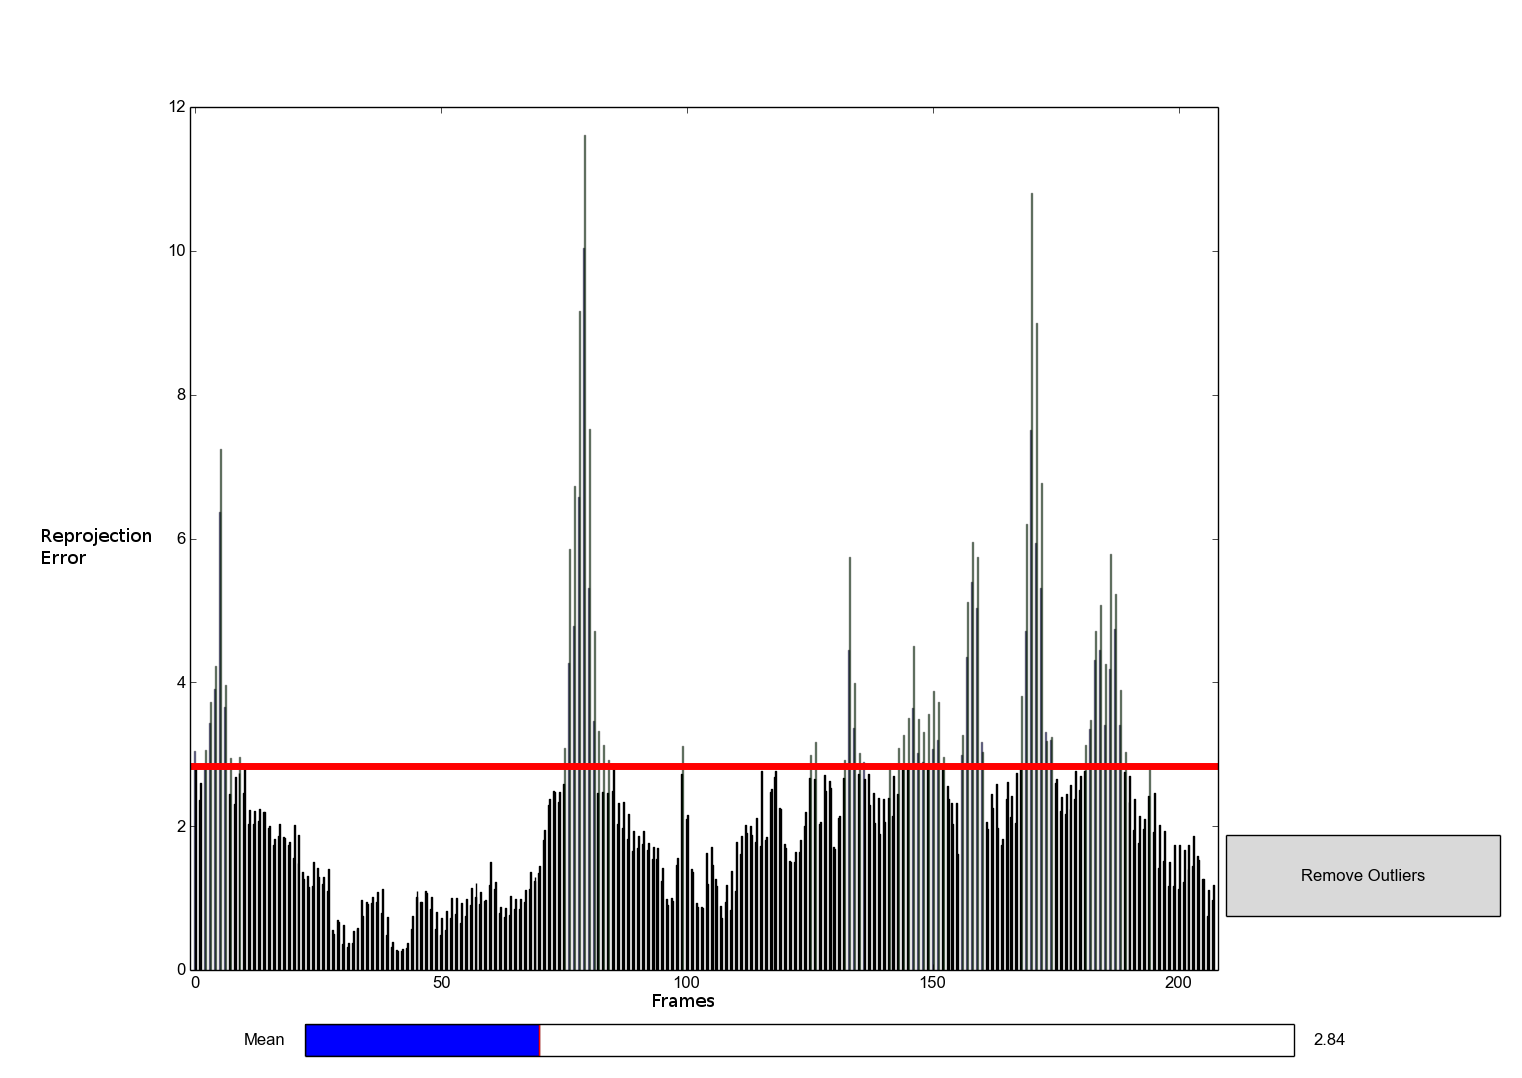
\includegraphics[width=0.95\textwidth]{./figures/allframes_axes_labels}}
	\caption{Initial reprojection errors plotted in python}
	\label{fig:cvrepro}
\end{figure}

\chapter{Stereo Shape Estimation}\label{chap:pcrecon}
\section{Overview}\label{sec:pcoverview}
Camera calibration was an important step in our overall pipeline of underwater cave reconstruction, because without it we could not accurately project 2\hyp D image points into 3\hyp D space. The footage for all of our tests were taken using a GoPro in SuperView mode, so this calibration problem needed to be addressed. With calibration out of the way, we now shift focus to the generation of a geometrically accurate point cloud using stereo footage collected in an underwater cave. The presented approach utilizes the presence of the artificial lighting to produce a rough model of the traversed area. In particular, the video\hyp light cone is used to identify the  walls of the cave from a single stereo pair. Furthermore, motion between consecutive stereo pairs is estimated and the 3\hyp D reconstruction is utilized to produce an approximate volumetric map of the cave.

\section{Related Work}\label{sec:pcrelwork}
The majority of underwater mapping up to now consists of fly\hyp overs with downward pointing sensors mapping the floor surface. The resulting representation consists of 2.5 dimensional mesh\hyp maps or image mosaics with minimal structure in the third dimension. In addition to underwater caves,  several other underwater environments  exhibit prominent three dimensional structure. Shipwrecks, are significant historical sites.  Producing accurate photorealistic 3\hyp D  models of these wrecks will assist in historical studies and also monitor their deterioration over time. During maritime disasters, it is important to produce accurate maps of the sunken vessel, especially the interior, in order to assist with rescue efforts. Multiple cases existed where survivors have been rescued from submerged vessels~\cite{Gray2003} hours, or even days after the event. Finally, underwater infrastructure inspection~\cite{Ribas2008} is another dangerous and tedious task that is required to be performed at regular intervals. Such infrastructure includes bridges, hydroelectric dams~\cite{Ridao2010}, water supply systems~\cite{White2010}, and oil rigs. For more information please refer to the Massot\hyp Campos and Oliver\hyp Codina survey~\cite{massot2015optical} for an overview of 3\hyp D sensing underwater. 

Most of the underwater navigation algorithms~\cite{lee2005underwater,snyder2010doppler,johannsson2010imaging,rigby2006towards} are based on acoustic sensors such as Doppler Velocity Log (DVL), ultra-short baseline (USBL) and sonar.  Gary et. al.~\cite{gary20083d} presented a 3D model of a cenote using LIDAR and sonar data collected by DEPTHX (DEep Phreatic THermal eXplorer) vehicle having DVL, IMU and depth sensor for underwater navigation. Corke et. al.~\cite{corke2007experiments} compared acoustic and visual methods for underwater localization. However, collecting data using DVL, sonar, and USBL while diving is expensive and sometimes not suitable in cave environments. 

Using stereo vision underwater has been proposed by several groups, however, most of the work has focused on open areas with natural lighting, or artificial light that completely illuminates the field of view. Small area dense reconstruction of a lit area was  proposed by Brandou et al.~\cite{Brandou2007}. Mahon et. al.~\cite{mahon2008efficient} proposed a SLAM algorithm based on the viewpoint augmented navigation (VAN) using stereo vision and DVL in underwater environment. A framework proposed by Leone et al.~\cite{Leone2008} operated over mainly flat surfaces. Several research groups have investigated the mapping and/or inspection of a ship's hull using different techniques~\cite{Hogue2007,Hover2007,Englot2013,akim-2013a}, the most famous shipwreck visual survey being that of the Titanic~\cite{Eustice2006}. Error analysis was performed recently by Sedlazeck and Koch \cite{Sedlazeck2012}. The problem of varying illumination was addressed by Nalpantidis et al.~\cite{Nalpantidis2010} for above\hyp ground scenes in stereo reconstruction. More recently, Servos, Smart and Waslander~\cite{Servos2013} presented a stereo SLAM algorithm with refraction correction in order to address the transitions between water, plastic, and air that exist in the underwater domain.
%\section{Related Work}\label{sec:pcrelwork}
The majority of underwater mapping up to now consists of fly\hyp overs with downward pointing sensors mapping the floor surface. The resulting representation consists of 2.5 dimensional mesh\hyp maps or image mosaics with minimal structure in the third dimension. In addition to underwater caves,  several other underwater environments  exhibit prominent three dimensional structure. Shipwrecks, are significant historical sites.  Producing accurate photorealistic 3\hyp D  models of these wrecks will assist in historical studies and also monitor their deterioration over time. During maritime disasters, it is important to produce accurate maps of the sunken vessel, especially the interior, in order to assist with rescue efforts. Multiple cases existed where survivors have been rescued from submerged vessels~\cite{Gray2003} hours, or even days after the event. Finally, underwater infrastructure inspection~\cite{Ribas2008} is another dangerous and tedious task that is required to be performed at regular intervals. Such infrastructure includes bridges, hydroelectric dams~\cite{Ridao2010}, water supply systems~\cite{White2010}, and oil rigs. For more information please refer to the Massot\hyp Campos and Oliver\hyp Codina survey~\cite{massot2015optical} for an overview of 3\hyp D sensing underwater. 

Most of the underwater navigation algorithms~\cite{lee2005underwater,snyder2010doppler,johannsson2010imaging,rigby2006towards} are based on acoustic sensors such as Doppler Velocity Log (DVL), ultra-short baseline (USBL) and sonar.  Gary et. al.~\cite{gary20083d} presented a 3D model of a cenote using LIDAR and sonar data collected by DEPTHX (DEep Phreatic THermal eXplorer) vehicle having DVL, IMU and depth sensor for underwater navigation. Corke et. al.~\cite{corke2007experiments} compared acoustic and visual methods for underwater localization. However, collecting data using DVL, sonar, and USBL while diving is expensive and sometimes not suitable in cave environments. 

Using stereo vision underwater has been proposed by several groups, however, most of the work has focused on open areas with natural lighting, or artificial light that completely illuminates the field of view. Small area dense reconstruction of a lit area was  proposed by Brandou et al.~\cite{Brandou2007}. Mahon et. al.~\cite{mahon2008efficient} proposed a SLAM algorithm based on the viewpoint augmented navigation (VAN) using stereo vision and DVL in underwater environment. A framework proposed by Leone et al.~\cite{Leone2008} operated over mainly flat surfaces. Several research groups have investigated the mapping and/or inspection of a ship's hull using different techniques~\cite{Hogue2007,Hover2007,Englot2013,akim-2013a}, the most famous shipwreck visual survey being that of the Titanic~\cite{Eustice2006}. Error analysis was performed recently by Sedlazeck and Koch \cite{Sedlazeck2012}. The problem of varying illumination was addressed by Nalpantidis et al.~\cite{Nalpantidis2010} for above\hyp ground scenes in stereo reconstruction. More recently, Servos, Smart and Waslander~\cite{Servos2013} presented a stereo SLAM algorithm with refraction correction in order to address the transitions between water, plastic, and air that exist in the underwater domain.
\section{Challenges}\label{sec:pcchallenges}



As can be seen in Fig. \ref{fig:caveLight}, the complete absence of natural illumination in combination with the presence of several sources of artificial illumination, such as: each diver's primary light and also one or more video\hyp lights, results in huge lighting variations in the scene. In particular each diver's primary light generates a tightly focused beam which is constantly moving with the motion of the diver. In Fig. \ref{fig:wireReco}a, there are three divers present: one holding the video light, his tanks visible at the bottom of the image; one traveling with the camera, not visible; and a third one whose DPV is visible at the top of the image. The primary light of the third diver can be seen as a blue beam pointing downwards, starting at the left of the DPV. 

\begin{figure*}[p]
	\begin{center}
		\leavevmode
		\begin{tabular}{ccc}
			\subfloat[]{\fbox{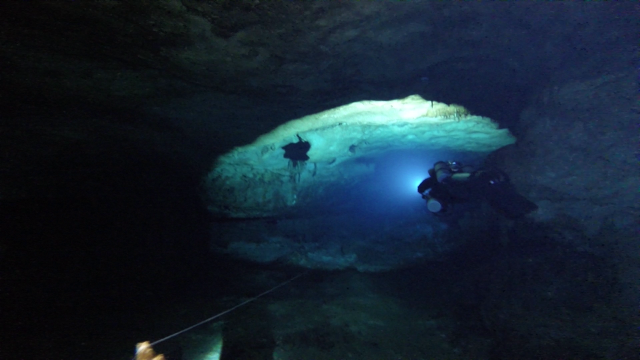
\includegraphics[width=0.62\textwidth]{figures/vlcsnap-2015-04-24-22h02m05s387S}\label{fig:light1}}}\\
			\subfloat[]{\fbox{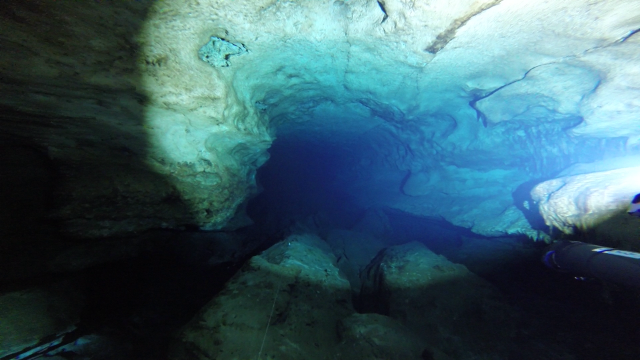
\includegraphics[width=0.62\textwidth]{figures/vlcsnap-2015-04-24-22h04m59s302S}\label{fig:light2}}}\\
			\subfloat[]{\fbox{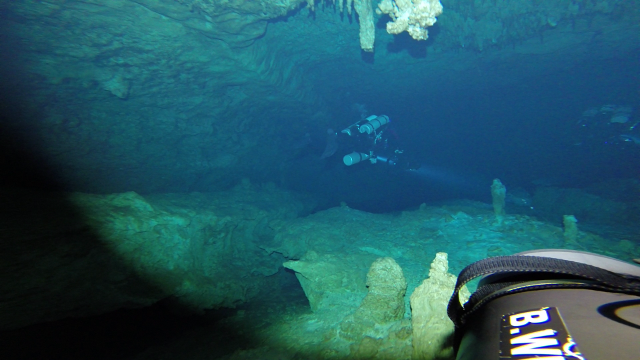
\includegraphics[width=0.62\textwidth]{figures/vlcsnap-2015-04-24-22h09m25s981S}\label{fig:light3}}} 
		\end{tabular}
	\end{center}
	\caption{Left camera images of an underwater cave with different illuminations. Illumination in the cave is provided by the lights individual divers have and also from a strong video\hyp light.  \ref{fig:light1}  Diver in front holds a strong video\hyp light; see how the cone of light outlines the boundaries of the cave. \ref{fig:light2}  Diver with video\hyp light follows behind the camera. \ref{fig:light3} The diver with the camera also holds the light.}
	\label{fig:caveLight}
\end{figure*}

\begin{figure*}[ht]
	\begin{center}
		\leavevmode
		\hspace*{-.2cm}\begin{tabular}{lll}
			\subfloat[]{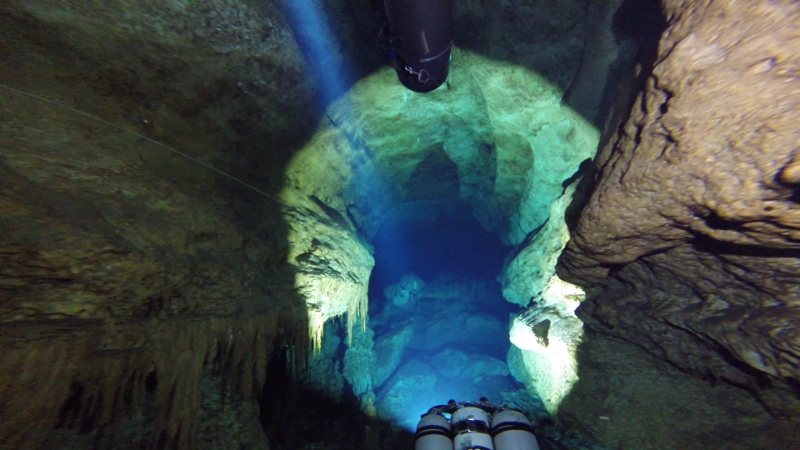
\includegraphics[width=0.47\textwidth]{figures/LUR_0000S}\label{fig:wire1}}&
			\subfloat[]{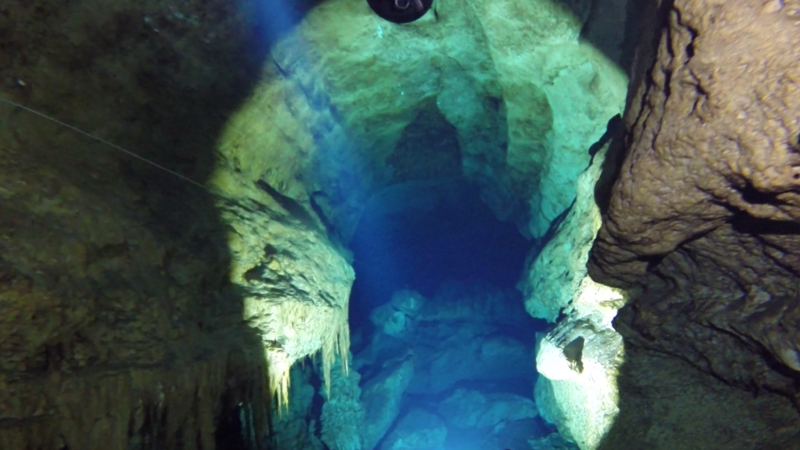
\includegraphics[width=0.47\textwidth]{figures/LR_0000RectS}\label{fig:wire2}}\\
			\subfloat[]{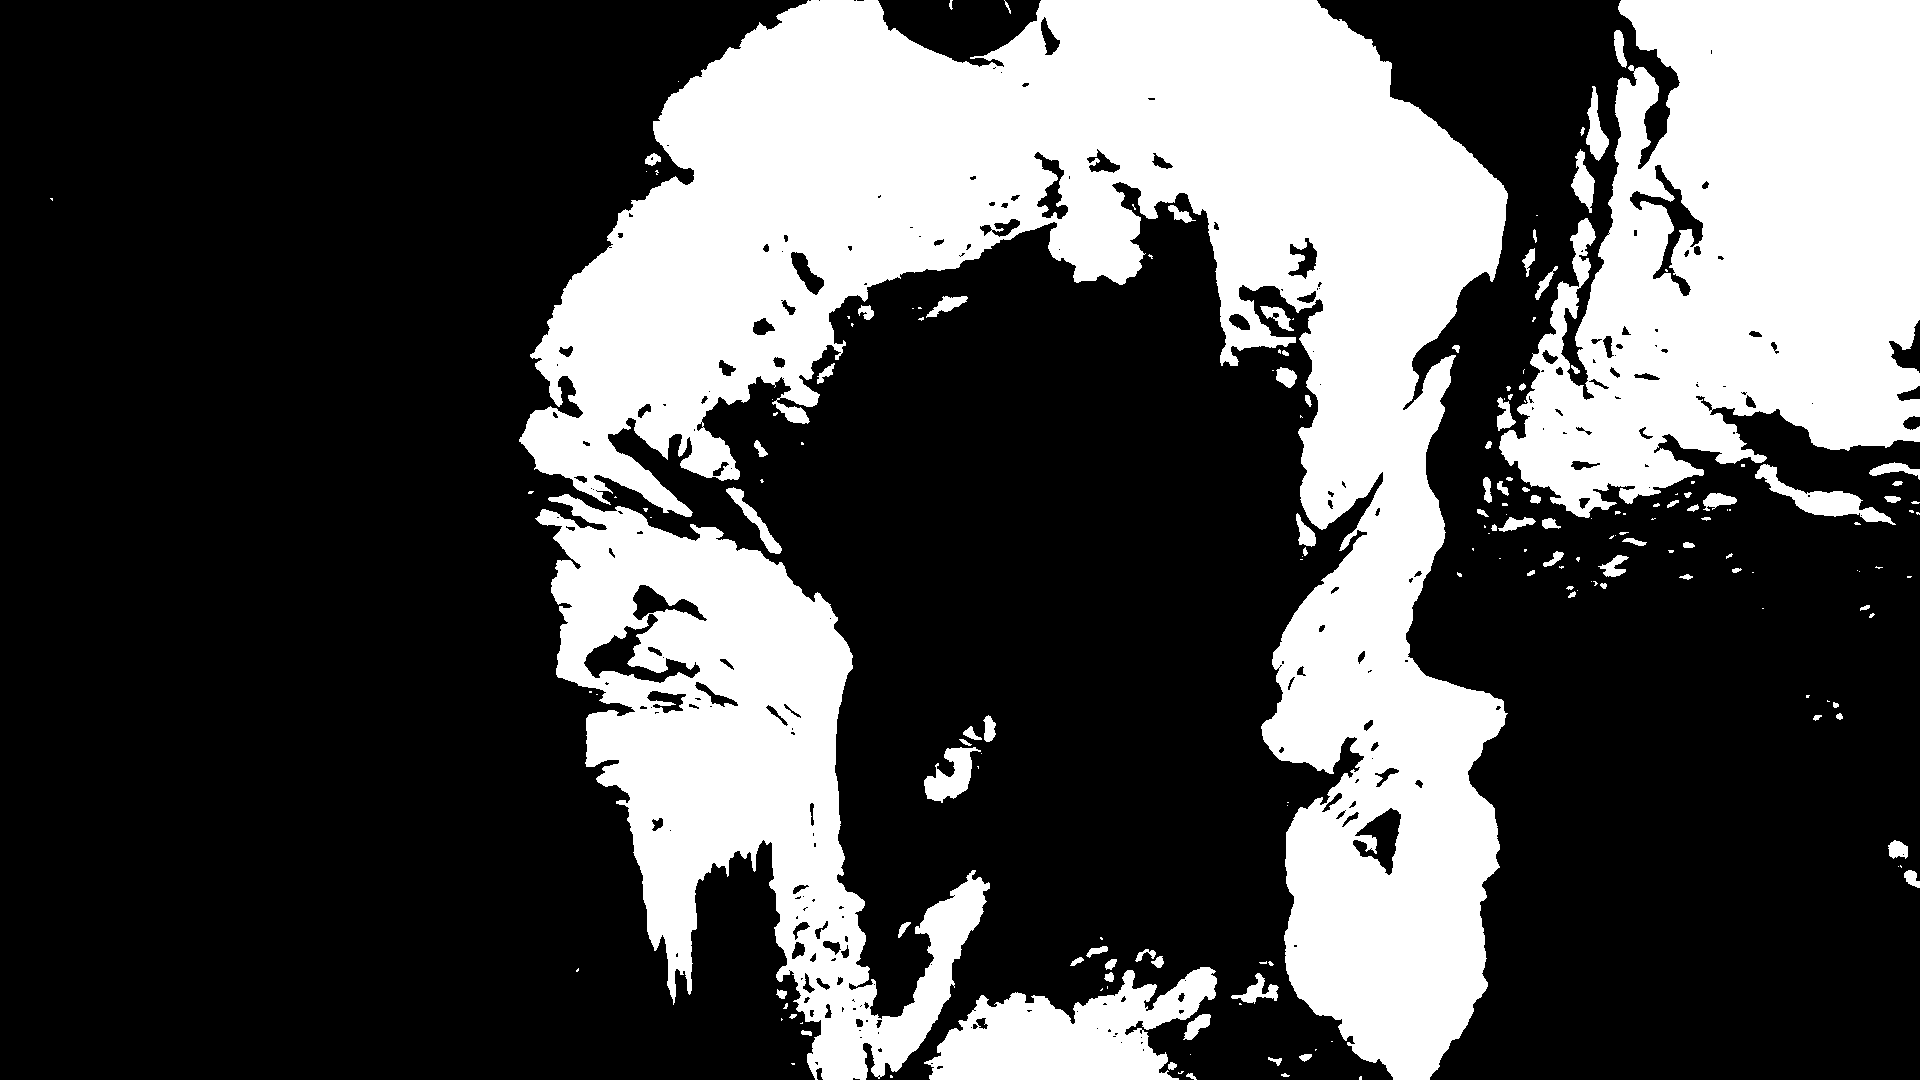
\includegraphics[width=0.47\textwidth]{figures/LT_0000Thr}\label{fig:wire3}}&
			\subfloat[]{\fbox{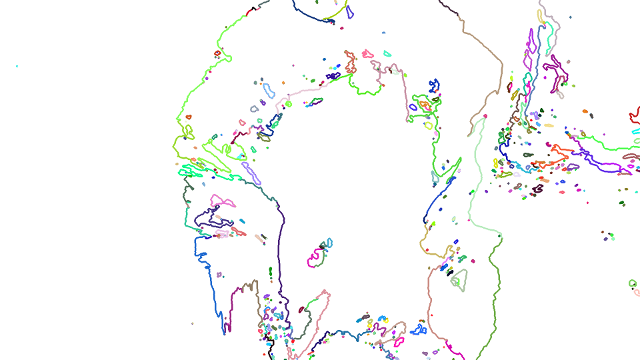
\includegraphics[width=0.47\textwidth]{figures/LT_0000EdgeS}\label{fig:wire4}}}\\
			\subfloat[]{\fbox{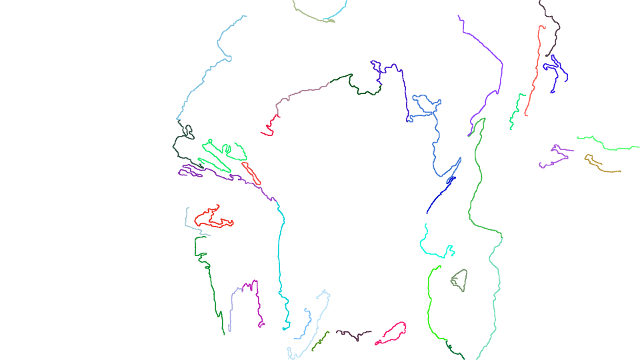
\includegraphics[width=0.47\textwidth]{figures/LT_0000FEdgeS}\label{fig:wire5}}}&
			\subfloat[]{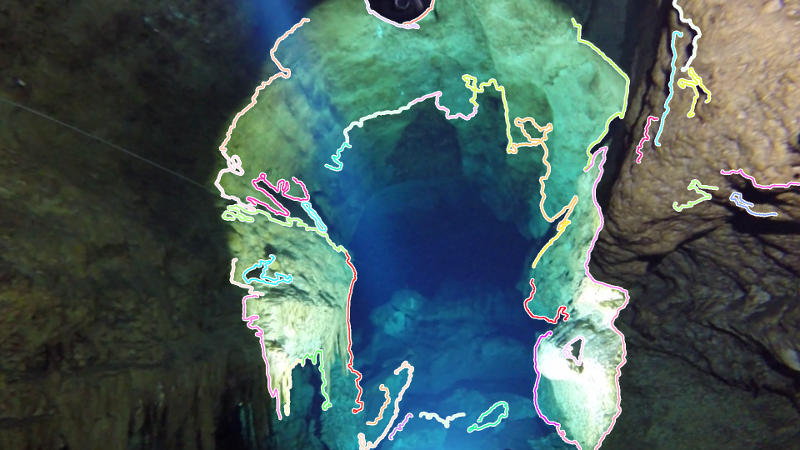
\includegraphics[width=0.485\textwidth]{figures/overlay_with_whiteS}\label{fig:wire6}}
		\end{tabular}
	\end{center}
	\caption{\ref{fig:wire1} Left camera image of an underwater cave.  \ref{fig:wire2} The rectified image. \ref{fig:wire3} The rectified image thresholded based on light intensity. \ref{fig:wire4} An edge map of the boundaries of the thresholded image. \ref{fig:wire5} The boundaries filtered to eliminate small contours. \ref{fig:wire6} The longer contours superimposed on the rectified image.}
	\label{fig:wireReco}
\end{figure*}

The lighting variations make the success of traditional visual odometry~\cite{nister2004visual} algorithms near impossible. The main assumption of Brightness Constancy Constraint underlying most visual odometry algorithms is violated by the constantly moving light\hyp sources. Table \ref{tab1} presents tests of five open source packages of vision based SLAM on underwater cave vision datasets; as expected most of them failed on the longer sequence and the rest were not able to extract the scale of the environment. It is worth noting that several of the packages are expecting specific motions in order to initialize~\cite{klein}. Complete results are not presented due to space constraints; interested readers should refer to the work of Quattrini Li et al.~\cite{RekleitisISERVO2016} for a detailed analysis of more packages and a variety of datasets. The selection of the algorithms presented here was motivated of testing a variety of methods; feature based~\cite{ORB1,4538852}, semi-direct~\cite{forster2014svo}, direct~\cite{raey}, and global~\cite{schoenberger2016sfm}. The main challenge these algorithms face is the constant change of the field of view and the dramatic lighting variations resulting from occlusions and from light absorption over distance. Among the most successful was the ORB\hyp SLAM~\cite{ORB1} with its latest incarnation as ORB\hyp SLAM 2, still in beta version, working with stereo images. While some of these packages, produced an acceptable trajectory, their shape reconstruction was plagued by noise.

%from the detected 3\hyp D features was plagued by noise.

\begin{table*}[htbp]
	\caption{Performance of different open source vision based SLAM packages on underwater data; for a detailed analysis please refer to Quattrini Li et al.~\cite{RekleitisISERVO2016}}
	\resizebox{\columnwidth}{!}{
		\begin{tabular}{|c|c|c|c|c|c|}
			\hline
			&\cite{ORB1}  &  \cite{4538852}&\cite{forster2014svo}  & \cite{raey} &\cite{schoenberger2016sfm}\\
			&ORB-SLAM  & PTAM & SVO & LSD-SLAM & Colmap\\
			\hline
			10 sec & noisy & no initialization & partial trajectories/no scale & loss of track & partial trajectories/no scale \\
			\hline 
			448 sec & noisy & no initialization  & partial trajectories/no scale  & loss of track  & partial trajectories/no scale  \\
			\hline
		\end{tabular}
	}
	\label{tab1}
\end{table*}%

\section{Wireframe Reconstruciton}\label{sec:pcwireframe}
Using light variations to infer shape has been used extensively in the past~\cite{Kender86shapefrom,Daum1998,Kutulakos2000}. The 3\hyp D reconstruction consists of several steps. First the images have to be rectified; a process achieved through a process called camera calibration. 

\paragraph*{Contour Tracking} Adaptive thresholding is used in order to identify the areas with different illumination; see  Fig. \ref{fig:wire3} for the thresholded image where the cone of the video\hyp light meets the cave walls. Selecting the right value for thresholding the image required some domain knowledge, and currently was perform per video sequence, by a human. Current experiments consider adjusting the threshold based on keeping a balance between the amount of light and dark areas, but that work is outside the scope of this paper.

During the next step, edge detection marks the boundaries between light and dark areas; see Fig. \ref{fig:wire4} for the boundaries of Fig. \ref{fig:wire2}. The OpenCV Canny edge detector~\cite{canny1986computational} is used to identify the edges marking the lighter area boundaries. As can be seen, the edge map is very noisy and thus not suitable for estimating the walls of the cave. A filter is applied to the contour list, eliminating  short contours. More specifically, for every contour, its bounding box is calculated and then only the highest fifth percentile is kept. While this method can eliminate elongated contours, experiments with the actual underwater cave video footage proved to not affect the main boundaries. The filtered contours can be seen in Fig. \ref{fig:wire5}. Figure \ref{fig:wire6} superimposes the filtered contours on the rectified image; the areas where the cone of light meets the cave walls are clearly identifiable. In addition, the area with acceptable lighting is  extracted for use at the motion estimation. The edge map of the boundaries is used then as input to a stereo reconstruction algorithm.

 \begin{figure}[h]
 	\centering
 	\fbox{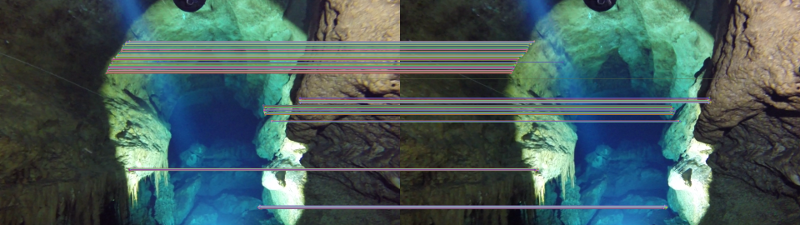
\includegraphics[width=.95\textwidth]{./figures/LT_0000_pngmatchesS}}
 	\caption{Select features matched at the boundary between left and right image of a stereo pair.}\vspace{-0.2in}
 	\label{fig:Matches}
 \end{figure}

\paragraph*{Sparse Stereo Reconstruction} The 3\hyp D structure of the cave boundaries is estimated for each stereo pair. For every point on the contour of the left image a SURF feature descriptor~\cite{Surf} is calculated using the left rectified image. Consequently, the same descriptor is matched on the right rectified image. Outlier rejection is facilitated by searching only locations at the same row and to the right of the left\hyp image feature's coordinates. As the camera calibration error is 0.8 pixels, it justifies the assumption above. Previous work on feature quality~\cite{ShiTomasi,Shkurti2011,RekleitisOceans2016} for underwater images indicated SURF~\cite{Surf} to be the most appropriate feature descriptor. Furthermore, the OpenCV Canny edge detector groups the edges in a list of continuous contours, as such consecutive points belonging to the same contour can be filtered for consistency.  Figure \ref{fig:Matches} presents select feature matches corresponding to the contours between the left and right image of a stereo pair.

\begin{figure*}[ht]
	\begin{center}
		\leavevmode
		\hspace*{-.2cm}\begin{tabular}{ccc}
			\subfloat[]{\fbox{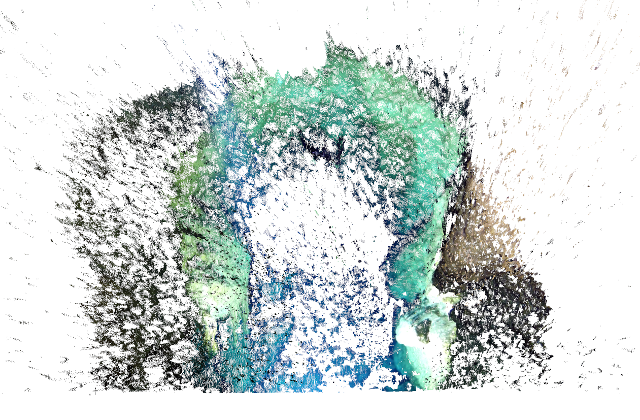
\includegraphics[height=0.14\textheight]{figures/sbm_straightS}}\label{fig:stereo1}}&
			\subfloat[]{\fbox{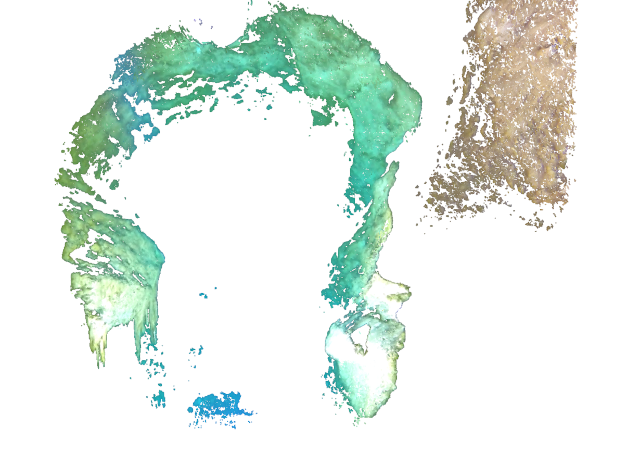
\includegraphics[height=0.14\textheight]{figures/threshold_straightS}}\label{fig:stereo2}}&
			\subfloat[]{\fbox{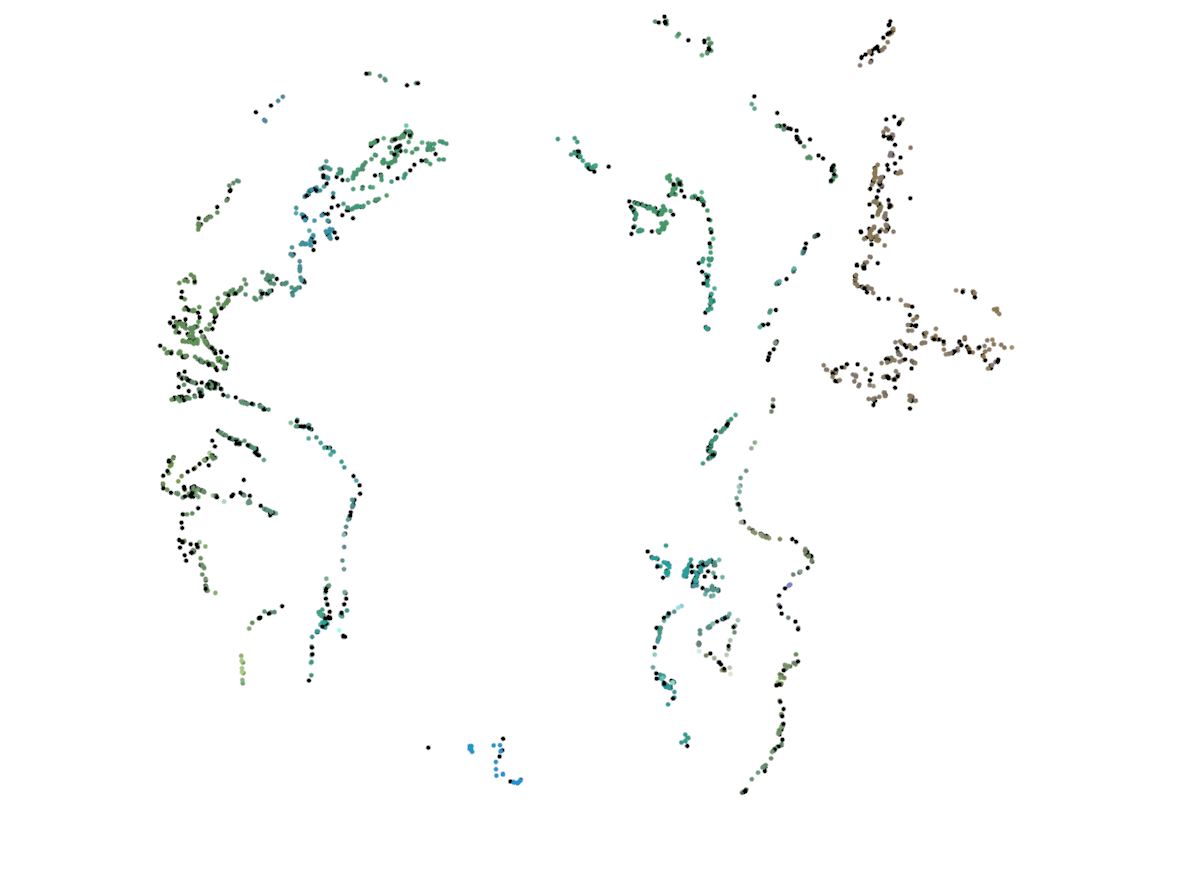
\includegraphics[height=0.14\textheight]{figures/contours_straight_larger}}\label{fig:stereo3}}\\
			\subfloat[]{\fbox{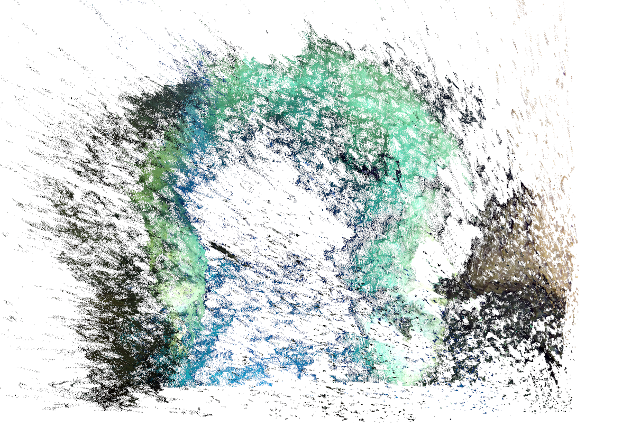
\includegraphics[height=0.14\textheight]{figures/sbm_shotgunS}}\label{fig:stereo4}}&
			\subfloat[]{\fbox{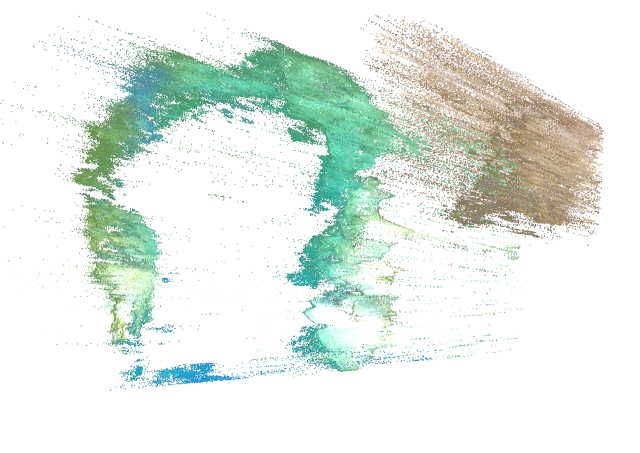
\includegraphics[height=0.14\textheight]{figures/threshold_shotgunS}}\label{fig:stereo5}}&
			\subfloat[]{\fbox{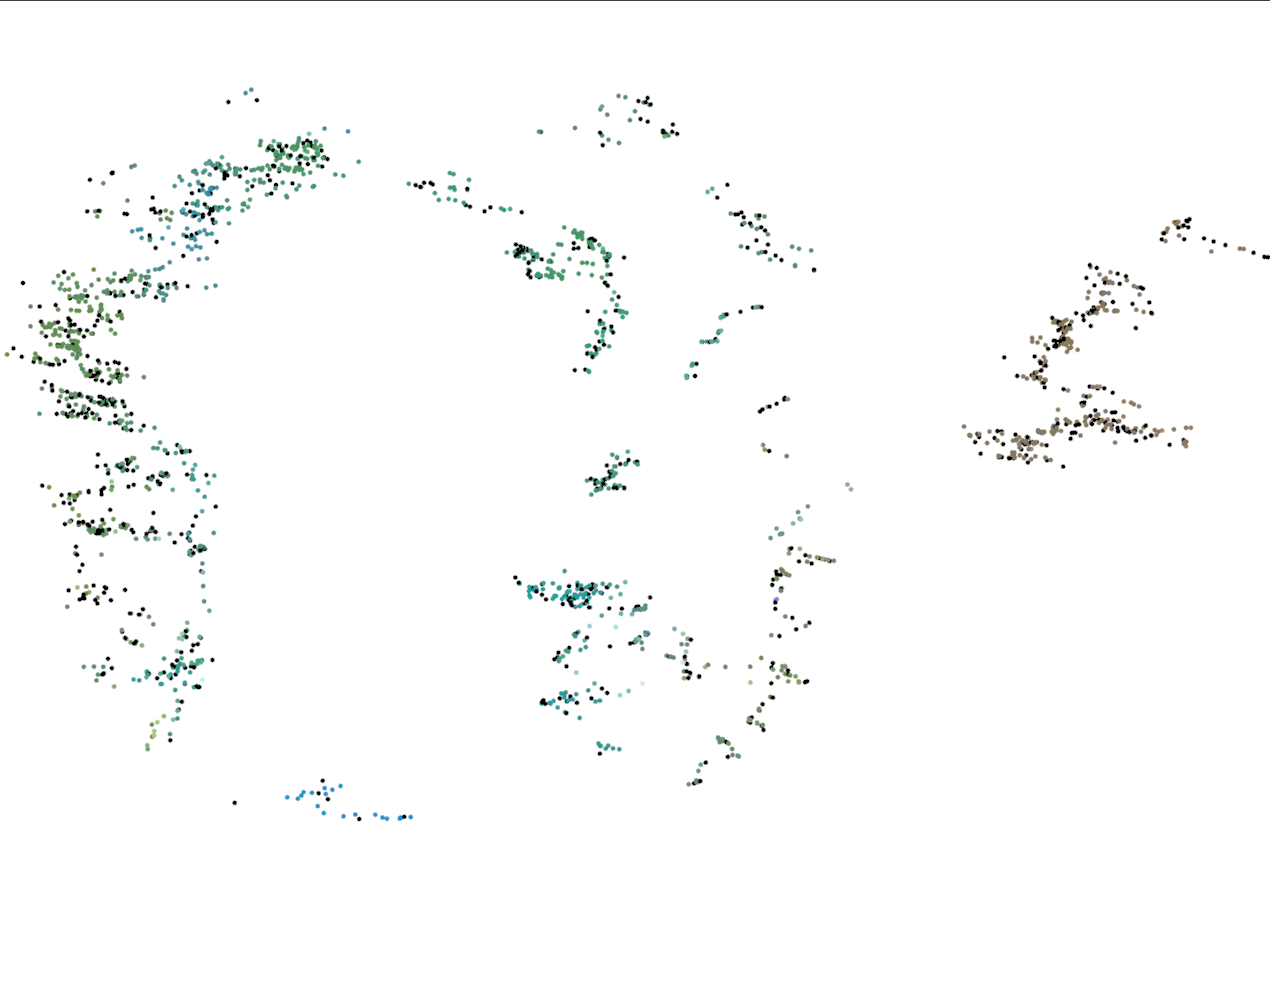
\includegraphics[height=0.14\textheight]{figures/contours_shotgun_larger}}\label{fig:stereo6}}
		\end{tabular}
	\end{center}
	\caption{Three different reconstructions from two different angles are presented. (a-c) Present a frontal view; (d-f) present a side view. \ref{fig:stereo1}, \ref{fig:stereo4} Disparity map of the Fig. \ref{fig:wire2} using the the OpenCV's semi-global block matching (SGBM) stereo algorithm.   \ref{fig:stereo2}, \ref{fig:stereo5} Applying the SGBM algorithm only to the lighted part.    \ref{fig:stereo3}, \ref{fig:stereo6} The contour in 3\hyp D using feature matches; see Fig. \ref{fig:Matches}. It is worth noting  elimination of outliers makes the contours much more distinct. }
	\label{fig:stereo}
\end{figure*}

Figure \ref{fig:stereo} presents a comparison of the performance of dense stereo reconstruction using OpenCV's semi-global block matching (SGBM) stereo algorithm~\cite{hirschmuller2008stereo} and the contour calculation. The standard output of dense stereo algorithms is a depth map, a normalized image where depth is quantified between 0 and 255; as such the values are discretized; see Figs. \ref{fig:stereo1},\ref{fig:stereo4} for the 3\hyp D reconstruction using the SGBM stereo algorithm on Fig. \ref{fig:wire2}. The noise is quite noticeable, Figs. \ref{fig:stereo2},\ref{fig:stereo5} present  the same reconstruction using only the lighted areas. Finally, Figs. \ref{fig:stereo3}, \ref{fig:stereo6} present  only the contours of high intensity variation extracted from Fig. \ref{fig:wire2} projected in 3\hyp D using SURF feature matching between left and right image. The noise is largely reduced, and the cave boundaries are clearly identifiable. While the first row of Fig. \ref{fig:stereo} presents a frontal view, and the error is not noticeable, the second row, presents a side view and the outliers are obvious. Currently, the corresponding points are calculated with pixel accuracy which results in disparity estimates that are integers. Consequently, the depth estimation is discretized and as it is inversely proportional to the distance of the camera there is a scattering effect. While this effect is strong during dense reconstructions, see Fig. \ref{fig:stereo3}, it is also present on the contour estimation; see Fig. \ref{fig:stereo4}
\section{Visual Odometry}\label{sec:pcvisodom}
 \begin{figure}[th]
 	\centering
 	\fbox{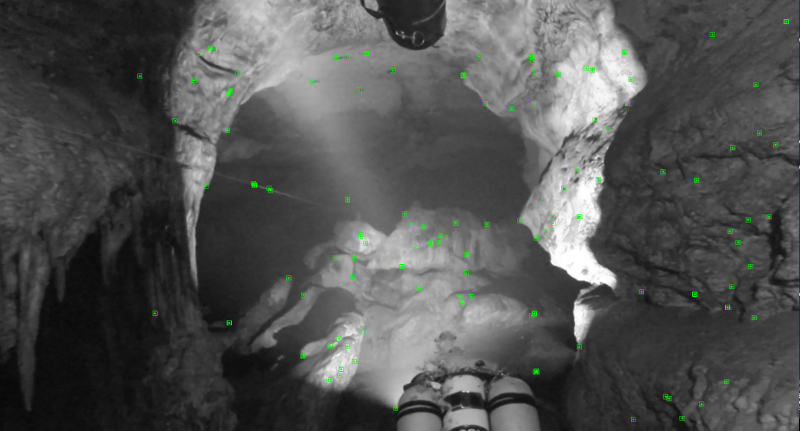
\includegraphics[width=0.9\textwidth]{./figures/OrbFeaturesS}}
 	\caption{ORB features tracked by ORB\hyp SLAM 2.}\vspace{-0.2in}
 	\label{fig:OrbFeatures}
\end{figure}

Brute force application of VO algorithms~\cite{da2009visual,Corke} is quite challenging in the underwater cave domain, due to the lighting variations and the sharp contrasts existing in the image, as discussed earlier. However, by thresholding the image, the areas of adequate illumination in the left and right camera feed can be used to apply one of the latest VO algorithms, ORB\hyp SLAM 2, a variant of ORB\hyp SLAM~\cite{ORB1,murTRO2015} for stereo vision. Figure \ref{fig:OrbFeatures} presents tracked features in the areas with higher illumination. It is worth noting that during some segments of the video the third diver swimming below the camera exhaled sending a cloud of bubbles in the field of view, however, the VO algorithm was robust enough to handle these dynamic features. This event highlighted one of the challenges of underwater vision. 

\begin{figure*}[ht]
	\begin{center}
		\leavevmode
		\begin{tabular}{cc}
			\subfloat[]{\fbox{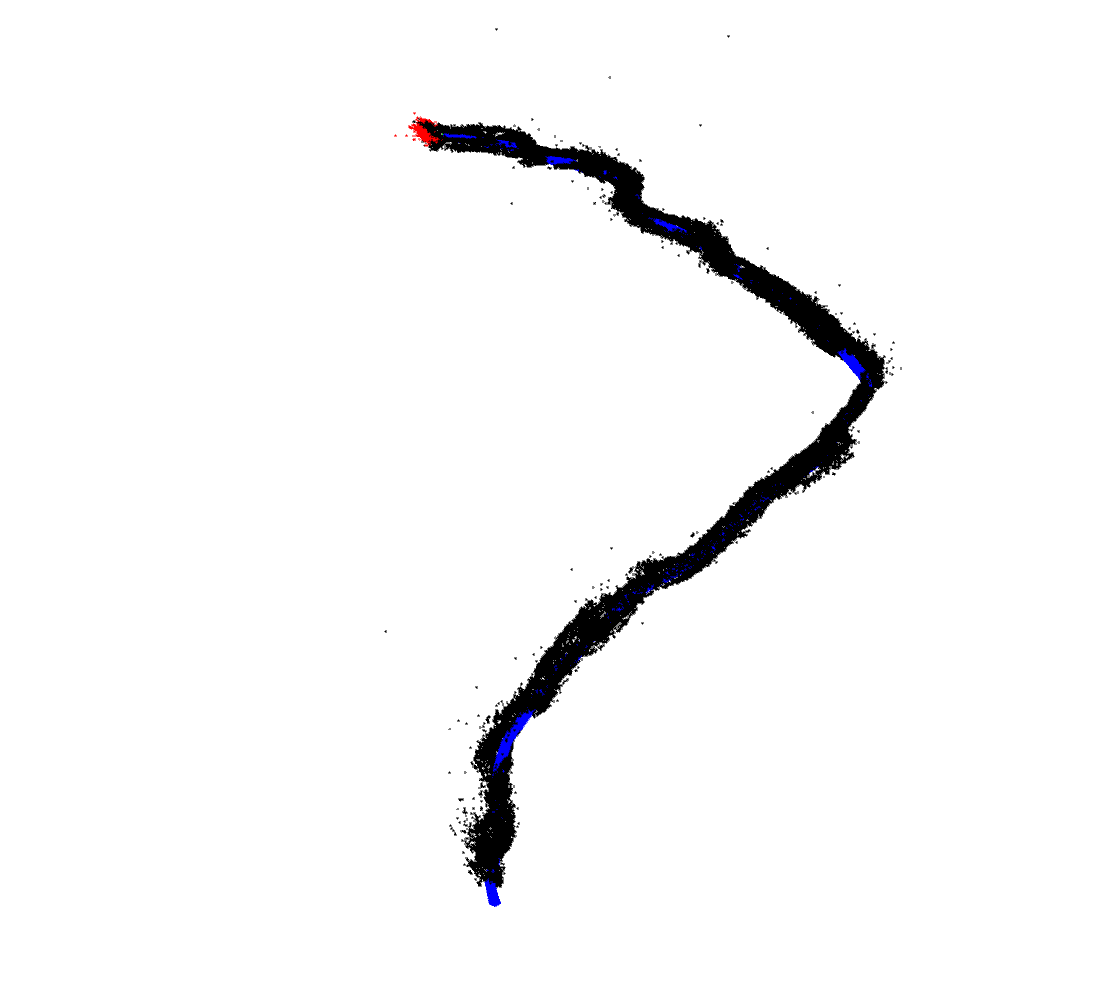
\includegraphics[height=0.41\textheight, clip=true, trim=3.0in 0.0in 2.0in 0.0in]{./figures/8_min_ORBSLAM}\label{fig:orb1}}}&
			\subfloat[]{\fbox{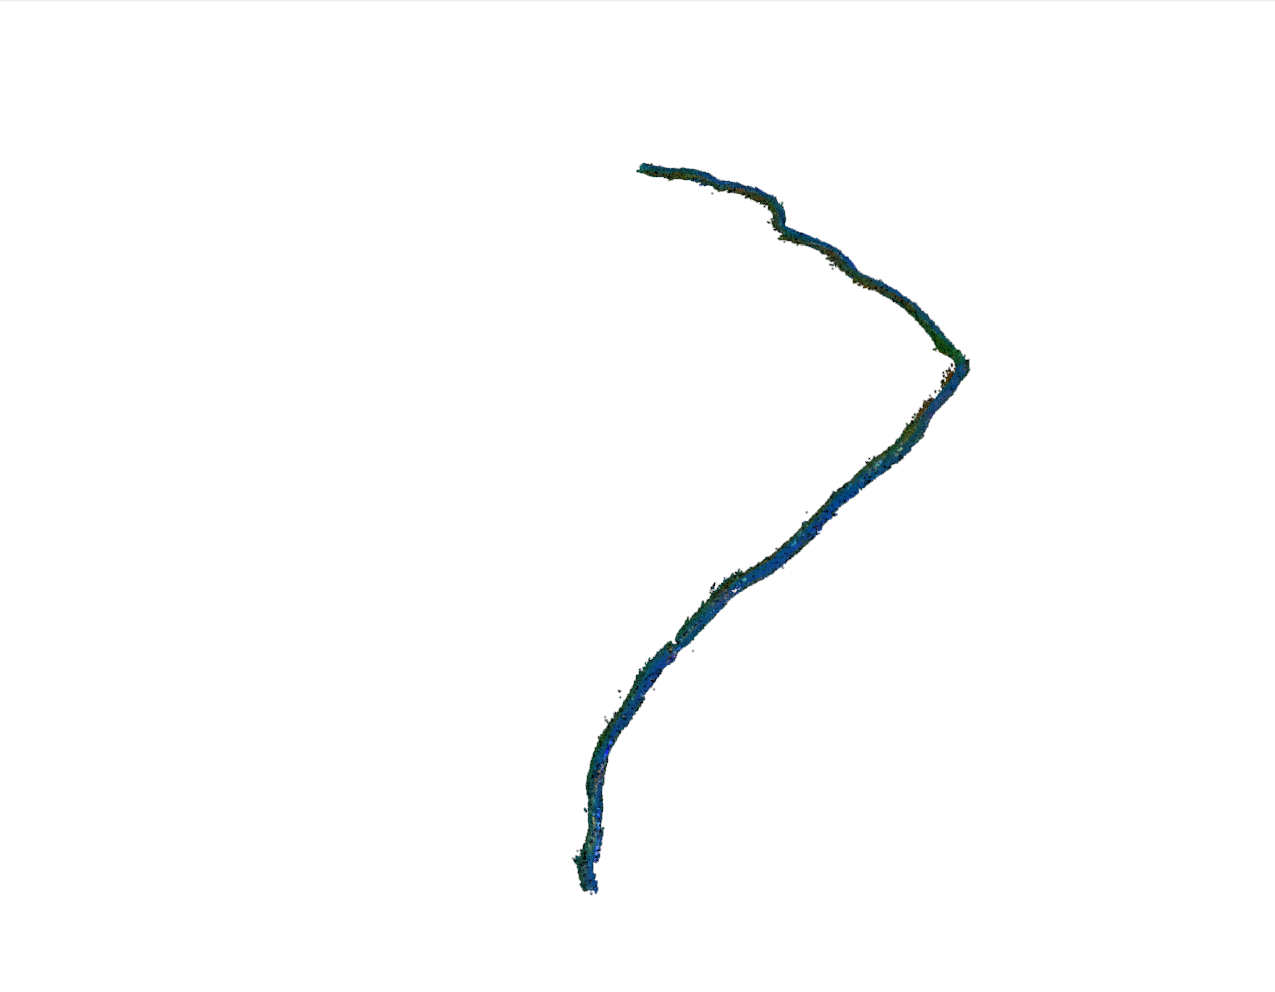
\includegraphics[height=0.41\textheight, clip=true, trim=5.0in 0.0in 2.50in 0.0in]{./figures/8_min_Our_Method}\label{fig:orb2}}}
		\end{tabular}
		\caption{\ref{fig:orb1} The trajectory calculated by ORB\hyp SLAM 2 of a 7 min 28 sec traversal and the 3\hyp D points estimated from ORB features. \ref{fig:orb2} The wireframe reconstructed from the proposed stereo algorithm. Please note, the reduced number of outliers compared to  \ref{fig:orb1}.}
		\label{fig:orb}
	\end{center}
\end{figure*}

Figure \ref{fig:orb} presents the trajectory of the stereo camera and the 3\hyp D position of stable features as extracted from ORB\hyp SLAM 2 from a trajectory of seven minutes, twenty eight seconds. While there was no ground truth, observing the video one gets a qualitative verification for the estimated trajectory. The estimated trajectory is then used as an input to produce a volumetric map by transforming the boundaries calculated above through space using the estimated pose of the stereo camera at each instant. It is clear that the contour based reconstruction; see Fig. \ref{fig:orb1}, has eliminated several outliers which were present in the ORB-SLAM reconstruction; see Fig. \ref{fig:orb2}. The next section presents results from an actual cave.
\section{Experimental Results}\label{sec:pcresults}
In January 2015, the authors requested from a cave exploration team in Mexico to acquire sample footage using a Dual Hero stereo camera from GoPro during a dive at an already explored cave. The selected cave is part of the Sistema Camilo, the 11th longest submerged cave system in the world, located at Quintana Roo, Yucatan peninsula, Mexico. The camera was mounted on a DPV and the video\hyp light was carried in different configurations in order to demonstrate alternative lighting schemes.

\paragraph*{Camera Calibration}As mentioned above, the stereo camera used utilizes a recording mode termed superview, which stretches the image in order to produce more aesthetically pleasing videos. Post\hyp processing all the calibration footage collected, error analysis showed, as expected, the error to slightly increase with distance; see Fig. \ref{fig:calError}. 

\begin{figure}[h]
	\begin{center}
		\leavevmode
		\hspace*{-.2cm}\begin{tabular}{cc}
			\subfloat[]{\fbox{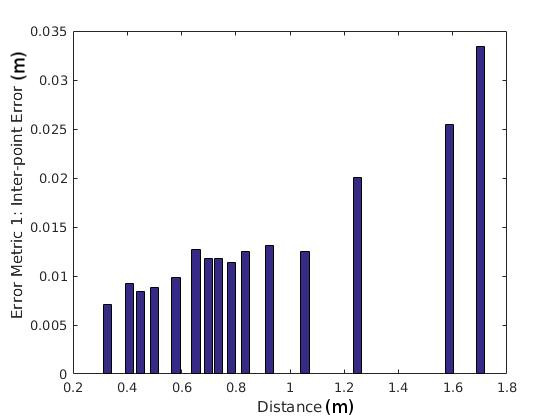
\includegraphics[width=0.47\textwidth]{./figures/error_metric1_edit.jpg}\label{fig:errMetric1}}}&
			\subfloat[]{\fbox{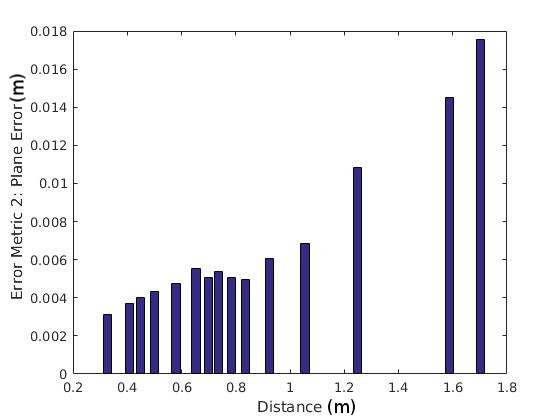
\includegraphics[width=0.47\textwidth]{./figures/error_metric2_edit.jpg}\label{fig:errMetric2}}}
		\end{tabular}
		\caption{\ref{fig:errMetric1} Average error of the inter-point distance of the target;  \ref{fig:errMetric2} Average error of the reconstructed points from the best plane fitting 3\hyp D points of the checkerboard. The results were from 4,000 images of the calibration target presented to the stereo camera underwater.}
		\label{fig:calError}
	\end{center}
\end{figure}

\paragraph*{Stereo Reconstruction}Figure \ref{fig:orb2} presents the 3\hyp D reconstruction of a long video of 7 min 28 sec. The structure corresponds with the cave morphology, however it is difficult to discern in the still image. Figure \ref{fig:tenSecDense} presents the 3\hyp D reconstruction of a cave segment from a short ten seconds traversal. The left and right walls are clearly identifiable, while the floor and ceiling are occluded from the two divers that swam in the field of view. 

\begin{figure*}[ht]
	\begin{center}
		\leavevmode
		\begin{tabular}{cc}
			\subfloat[]{{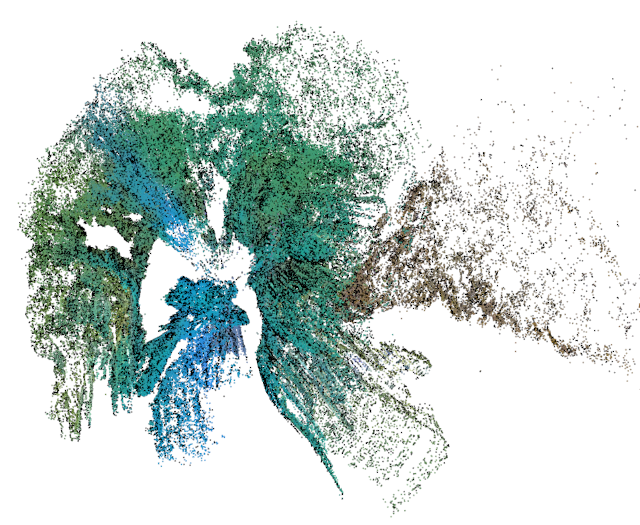
\includegraphics[width=0.75\textwidth]{./figures/dense_10sec_outsideS}\label{fig:ten1}}}\\
			\subfloat[]{{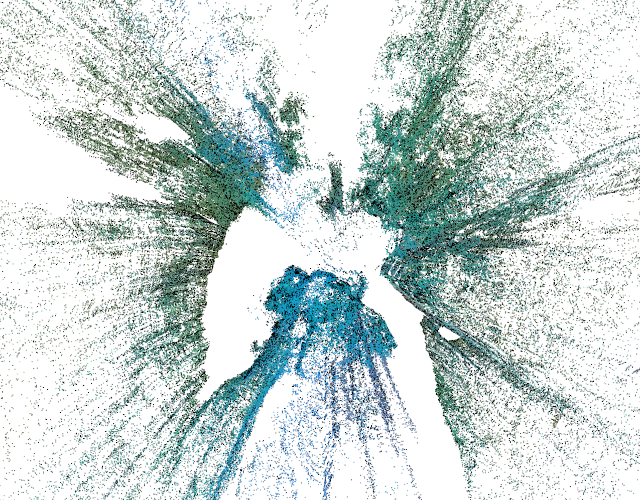
\includegraphics[width=0.75\textwidth]{./figures/dense_10sec_insideS}\label{fig:ten2}}}
		\end{tabular}
		\caption{\ref{fig:ten1} The 3\hyp D walls of the cave extracted from a short ten second traversal. \ref{fig:ten2} A second view more inside the reconstruction.}
		\label{fig:tenSecDense}
	\end{center}
\end{figure*}

\chapter{Surface Reconstruction}\label{chap:srecon}
\section{Overview}\label{sec:reconoverview}
A geometrically sound point cloud gives a lot of information about the 3\hyp D structure of cave. The shape can be easily inferred, and features of the cave such as stalagmites take shape. It is also easy to see how the cave system is shaped on a large scale when longer segments are constructed such as in \ref{fig:orb}. What a point cloud lacks though is information between all of the points. This space can be either large or small depending on the how many image frames were used to build the model. These empty spaces can cause visual problems if shapes loose their definition due to lack of information. If these models were to be used for robot integration as discussed earlier, the area of these holes cannot be used for any kind of sensing information. Due to this need for additional information in our reconstructed model, surface reconstruction is used in order to fill the empty spaces. Our reconstruction problem is not unique enough to warrant a brand new surface reconstruction technique. As will be explained in section \ref{sec:reconrelwork}, a lot of work has gone into the problem of surface reconstruction. We hope to identify the best method out there for our particular problem, and build upon those results to refine our final output even more. 

%The goal is a reconstruction of a full model that continuously defines the shape of the cave structure and overlays texture information to give visual definition to the shape.

\section{Related Work}\label{sec:reconrelwork}
Surface reconstruction is a problem that expands well beyond scene reconstruction from a camera. Many methods have developed for data collected with range scan datasets. Luckily these methods can often be applied generically to any kind of data set, but there are key components and limiting factors that make some better than others. Such data sets as those collected with underwater stereo images often fail under the constraints of popularized techniques. 

A subcategory of surface reconstruction techniques is that of point interpolation. In this category, the input data points would all represent points exactly on the surface of the reconstruction object. Because this is  in practice impossible without at least some minimal error, applications take measurement error into account, but assume it to be small. These methods are thus popular on range scan data sets where the volume of the data points is high, the surface is usually smooth, and the degree of error is often small. Popular methods include the cocone method~\cite{amenta2000simple} and the power crust method~\cite{amenta2001power} which use a piecewise linear approximation of the surface based on a Delaunay triangulation of the input points. Alternatively there is the ball-pivoting algorithm~\cite{817351}  which incrementally builds a surface based on the idea of a ball rolling across and intersecting points. These methods are also incredibly susceptible to noise due to their assumption that the points exactly lie on the object surface. This can mitigated by noise smoothing or popular point sampling techniques such as Poisson disk sampling~\cite{corsini2012efficient}, but the loss of data can result in an output to abstract from the true reconstruction. 

Alternative to point interpolation, there is also the category of algorithms that deal with point approximation. This removes the restriction that points must lie on the on the reconstruction object, and the methods are much more varied. Many of these techniques require knowledge of the point normals, which is absent information when generating input points from images. Thus methods have developed for determining and orienting the normals of points based on estimating the normal of a plane tangent to the surface~\cite{RusuDoctoralDissertation}. Known point normal information now introduces the use of approximation reconstruction techniques. Signed distance function approaches such as those developed by Hoppe et al.~\cite{Hoppe:1992:SRU:133994.134011,Hoppe:1995:SRU:221616} define a surface in implicit form and then allow for the extraction of a final triangulated mesh using popular approaches such as marching cubes~\cite{Lorensen:1987:MCH:37401.37422}. Instead of using a distance function, methods such as Poisson reconstruction~\cite{Kazhdan:2006:PSR:1281957.1281965} use indicator functions to define a water tight model. Lastly there are approaches using moving least-squares(MLS) which were introduced by Levin~\cite{levin2004mesh} and soon popularized through point set surfaces by Alexa et al.~\cite{alexa2003computing} All together these form a vast library of surface reconstruction techniques to use between the interpolation and approximation subcategories. 

With such a large volume of available solutions to the surface reconstruction problem, it is important to identify the best approach given a specific data set. In our case we need to identify a method that can deal with the sparsity of our point cloud volume while also not falling susceptible to noise. Other works have done similar data collection and reconstruction of underwater systems using cameras as their primary means of data collection. Johnson-Roberson et al.~\cite{johnson2010generation} used Delaunay triangulation to reconstruct individual top down stereo images of the sea floor. These individual reconstructions are then aggregated together using a Volumetric Range Image Processing (VRIP) technique developed by Curless and Levoy. Campos et al.~\cite{campos2014surface} introduced a method for 3D surface reconstruction with an emphasis on underwater optical mapping. This method is inspired by restricted Delaunay triangulation and is robust to noise and outliers often attributed with underwater data collection. Unfortunately these two methods have clear advantages. The former only scans directly below at the more or less flat ocean floor, while the latter builds a point set from a large collection of camera angles and locations. Another study by Tischenko~\cite{tishchenko_2010} used a range scan and collected data out of water, but compared the best approaches to reconstructing a hollow cylindrical point cloud shape. This is similar to the shape of our cave system and can thus prove useful. This study found the marching cubes implementation mentioned earlier by Hoppe to produce the most accurate reconstruction results. 


%Solutions to surface reconstruction from point clouds vary depending on the domain and the input data. Factors such as the density of the cloud, the kind of preliminary structural data coinciding with the cloud, and the noise of the cloud all define the approach used in reconstruction. Our method for point cloud generation creates a cylindrical shape for the cave at both a sparse and dense level depending on the number of input frames used. In both cases the cloud contains noise and lacks any predefined data on the values for the point normals. Previous work by Tishchenko ~\cite{tishchenko_2010} compares the advantages of certain surface reconstruction algorithms, and while the input clouds were generated above water and using a laser, they share the properties of forming a cylindrical shape without point normals and noise present. These comparisons highlight a method for calculating point normals based on point neighborhoods and distinguish a Marching Cubes surface reconstruction method by Hoppe as the appropriate approach to a problem with these parameters~\cite{Hoppe:1992:SRU:133994.134011,Hoppe:1995:SRU:221616}. Other techniques such as Poisson surface reconstruction and Delaunay triangulation are used heavily in the underwater domain ~\cite{campos2014surface}. 
%
%A powerful tool for implementing surface reconstruction techniques is the open source application Meshlab. Meshlab includes implementation of normal estimation, marching cubes ~\cite{guennebaud2008dynamic}, and Poisson reconstruction ~\cite{Kazhdan:2006:PSR:1281957.1281965}. It also includes an implementation of the Ball-Pivoting Algorithm ~\cite{mittlemanball} that produces interesting results, while still succumbing to the drawbacks highlighted in Tishchenko's comparison. Lastly, Meshlab also has an implementation of Poisson-disk sampling ~\cite{corsini2012efficient}. Sampling of point cloud sets allows reconstruction algorithms to avoid noise errors and unnecessary over fitting, but the dsrawback is a loss of accuracy from the volume of input points. Sampling has a varying effect on the output depending on the algorithm, and in cases of Ball-Pivoting the results are highly dependent on it. A challenge for all of these algorithms is that they rely on a set of input parameters that can vary the output. Finding the proper parameters introduces another level of complexity to outputting an accurate final mesh.
%\section{Related Work}\label{sec:reconrelwork}
Surface reconstruction is a problem that expands well beyond scene reconstruction from a camera. Many methods have developed for data collected with range scan datasets. Luckily these methods can often be applied generically to any kind of data set, but there are key components and limiting factors that make some better than others. Such data sets as those collected with underwater stereo images often fail under the constraints of popularized techniques. 

A subcategory of surface reconstruction techniques is that of point interpolation. In this category, the input data points would all represent points exactly on the surface of the reconstruction object. Because this is  in practice impossible without at least some minimal error, applications take measurement error into account, but assume it to be small. These methods are thus popular on range scan data sets where the volume of the data points is high, the surface is usually smooth, and the degree of error is often small. Popular methods include the cocone method~\cite{amenta2000simple} and the power crust method~\cite{amenta2001power} which use a piecewise linear approximation of the surface based on a Delaunay triangulation of the input points. Alternatively there is the ball-pivoting algorithm~\cite{817351}  which incrementally builds a surface based on the idea of a ball rolling across and intersecting points. These methods are also incredibly susceptible to noise due to their assumption that the points exactly lie on the object surface. This can mitigated by noise smoothing or popular point sampling techniques such as Poisson disk sampling~\cite{corsini2012efficient}, but the loss of data can result in an output to abstract from the true reconstruction. 

Alternative to point interpolation, there is also the category of algorithms that deal with point approximation. This removes the restriction that points must lie on the on the reconstruction object, and the methods are much more varied. Many of these techniques require knowledge of the point normals, which is absent information when generating input points from images. Thus methods have developed for determining and orienting the normals of points based on estimating the normal of a plane tangent to the surface~\cite{RusuDoctoralDissertation}. Known point normal information now introduces the use of approximation reconstruction techniques. Signed distance function approaches such as those developed by Hoppe et al.~\cite{Hoppe:1992:SRU:133994.134011,Hoppe:1995:SRU:221616} define a surface in implicit form and then allow for the extraction of a final triangulated mesh using popular approaches such as marching cubes~\cite{Lorensen:1987:MCH:37401.37422}. Instead of using a distance function, methods such as Poisson reconstruction~\cite{Kazhdan:2006:PSR:1281957.1281965} use indicator functions to define a water tight model. Lastly there are approaches using moving least-squares(MLS) which were introduced by Levin~\cite{levin2004mesh} and soon popularized through point set surfaces by Alexa et al.~\cite{alexa2003computing} All together these form a vast library of surface reconstruction techniques to use between the interpolation and approximation subcategories. 

With such a large volume of available solutions to the surface reconstruction problem, it is important to identify the best approach given a specific data set. In our case we need to identify a method that can deal with the sparsity of our point cloud volume while also not falling susceptible to noise. Other works have done similar data collection and reconstruction of underwater systems using cameras as their primary means of data collection. Johnson-Roberson et al.~\cite{johnson2010generation} used Delaunay triangulation to reconstruct individual top down stereo images of the sea floor. These individual reconstructions are then aggregated together using a Volumetric Range Image Processing (VRIP) technique developed by Curless and Levoy. Campos et al.~\cite{campos2014surface} introduced a method for 3D surface reconstruction with an emphasis on underwater optical mapping. This method is inspired by restricted Delaunay triangulation and is robust to noise and outliers often attributed with underwater data collection. Unfortunately these two methods have clear advantages. The former only scans directly below at the more or less flat ocean floor, while the latter builds a point set from a large collection of camera angles and locations. Another study by Tischenko~\cite{tishchenko_2010} used a range scan and collected data out of water, but compared the best approaches to reconstructing a hollow cylindrical point cloud shape. This is similar to the shape of our cave system and can thus prove useful. This study found the marching cubes implementation mentioned earlier by Hoppe to produce the most accurate reconstruction results. 


%Solutions to surface reconstruction from point clouds vary depending on the domain and the input data. Factors such as the density of the cloud, the kind of preliminary structural data coinciding with the cloud, and the noise of the cloud all define the approach used in reconstruction. Our method for point cloud generation creates a cylindrical shape for the cave at both a sparse and dense level depending on the number of input frames used. In both cases the cloud contains noise and lacks any predefined data on the values for the point normals. Previous work by Tishchenko ~\cite{tishchenko_2010} compares the advantages of certain surface reconstruction algorithms, and while the input clouds were generated above water and using a laser, they share the properties of forming a cylindrical shape without point normals and noise present. These comparisons highlight a method for calculating point normals based on point neighborhoods and distinguish a Marching Cubes surface reconstruction method by Hoppe as the appropriate approach to a problem with these parameters~\cite{Hoppe:1992:SRU:133994.134011,Hoppe:1995:SRU:221616}. Other techniques such as Poisson surface reconstruction and Delaunay triangulation are used heavily in the underwater domain ~\cite{campos2014surface}. 
%
%A powerful tool for implementing surface reconstruction techniques is the open source application Meshlab. Meshlab includes implementation of normal estimation, marching cubes ~\cite{guennebaud2008dynamic}, and Poisson reconstruction ~\cite{Kazhdan:2006:PSR:1281957.1281965}. It also includes an implementation of the Ball-Pivoting Algorithm ~\cite{mittlemanball} that produces interesting results, while still succumbing to the drawbacks highlighted in Tishchenko's comparison. Lastly, Meshlab also has an implementation of Poisson-disk sampling ~\cite{corsini2012efficient}. Sampling of point cloud sets allows reconstruction algorithms to avoid noise errors and unnecessary over fitting, but the dsrawback is a loss of accuracy from the volume of input points. Sampling has a varying effect on the output depending on the algorithm, and in cases of Ball-Pivoting the results are highly dependent on it. A challenge for all of these algorithms is that they rely on a set of input parameters that can vary the output. Finding the proper parameters introduces another level of complexity to outputting an accurate final mesh.
\section{Algorithm Comparison}\label{sec:reconalgcomp}
From a surface reconstruction perspective, the point clouds generated from our light ring model have a number of important characteristics. The only data outputted by stereo matching is the (x,y,z) coordinates of the image points in space with respect to their relative camera poses. These points can additionally coincide with RGB values from the image, but due to the nature of our data collected the colors are always some of the highest intensity pixel values and thus much of the texture detail is lost. Because no other data is currently saved with the point data, we lack information about the point normals. At the same time, there are often outlier points that make it to the stereo matching phase. One advantage of our method is that since we only project points on the ring of light which should be in a different location every frame, theoretically our points should have limited overlap. With these problem specifics and constraints defined, the task now becomes identifying a proper surface reconstruction technique to form our initial base mesh.

For the sake of rapid prototyping different reconstruction methods on our data set, tests were run using the application Meshlab. Meshalb has a number of the techniques discussed in \ref{sec:reconrelwork} built in making it a quick option for comparing the outputs. Tests run in Meshlab could not be integrated into our pipeline, but they helped identify the proper procedure. 

Our pipeline renders our point cloud using the Point Cloud Library(PCL). PCL has a number of additional functionalities that can help in the reconstruction phase. First off, statistical outlier removal can be applied to our points. Mean distances are computer for each point in regards to its neighboring points. Points whose mean distances exceed that of the global mean and standard deviation are labeled outliers and removed from the set. This eliminates points that were picked up by the feature detector in  the image processing stage, but whos spacial position would only distort the final reconstruction. Second, we can apply the normal calculation and orientation described in \ref{sec:reconrelwork}. The points we projected from the image are all on the inside of the cave, so all of the normals should be oriented inwards. PCL makes the assumption that normals are oriented towards the camera, which is exactly what we want since our camera moves through the inside of the cave. A subset of the resulting normals can be seen in \ref{fig:showing_normals}.

\begin{figure*}[ht]
	\begin{center}
		\leavevmode
		\begin{tabular}{cc}
			\subfloat[]{{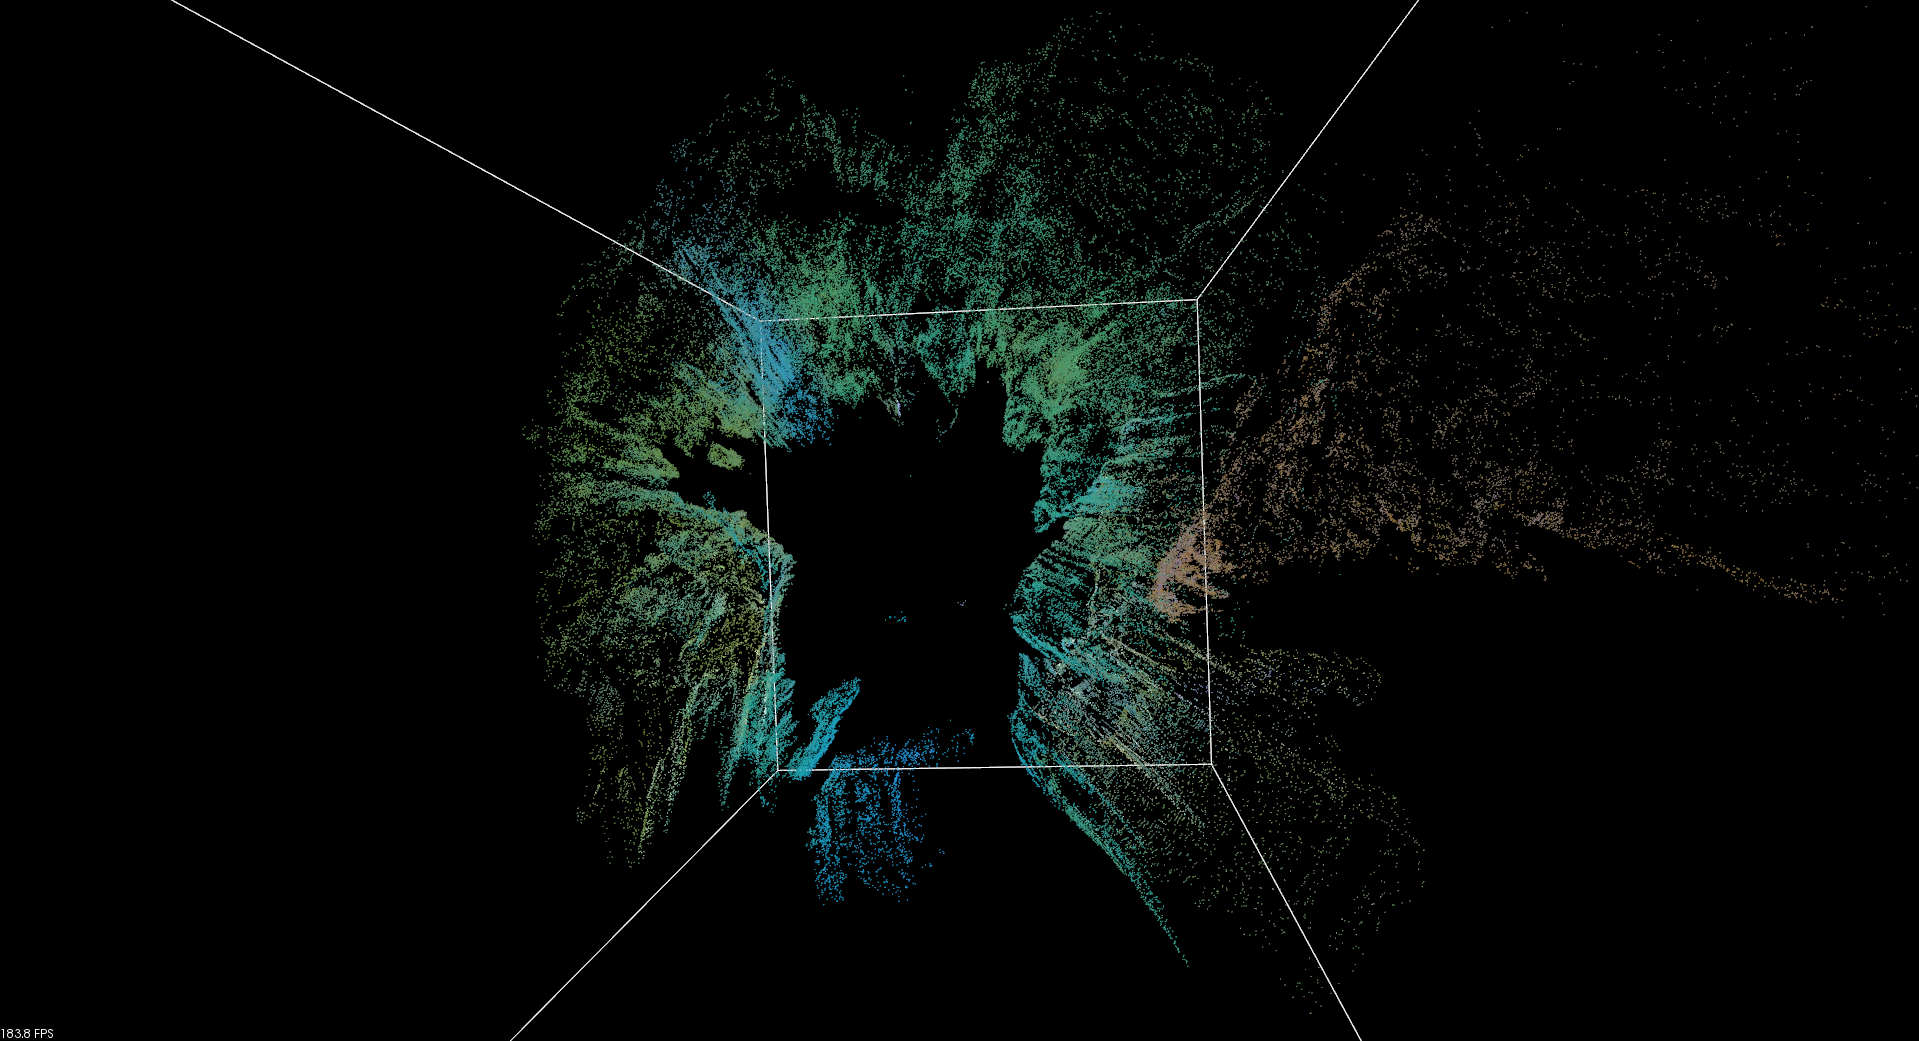
\includegraphics[width=0.95\textwidth]{./figures/normals_pcl_without}\label{fig:without_normals}}}\\
			\subfloat[]{{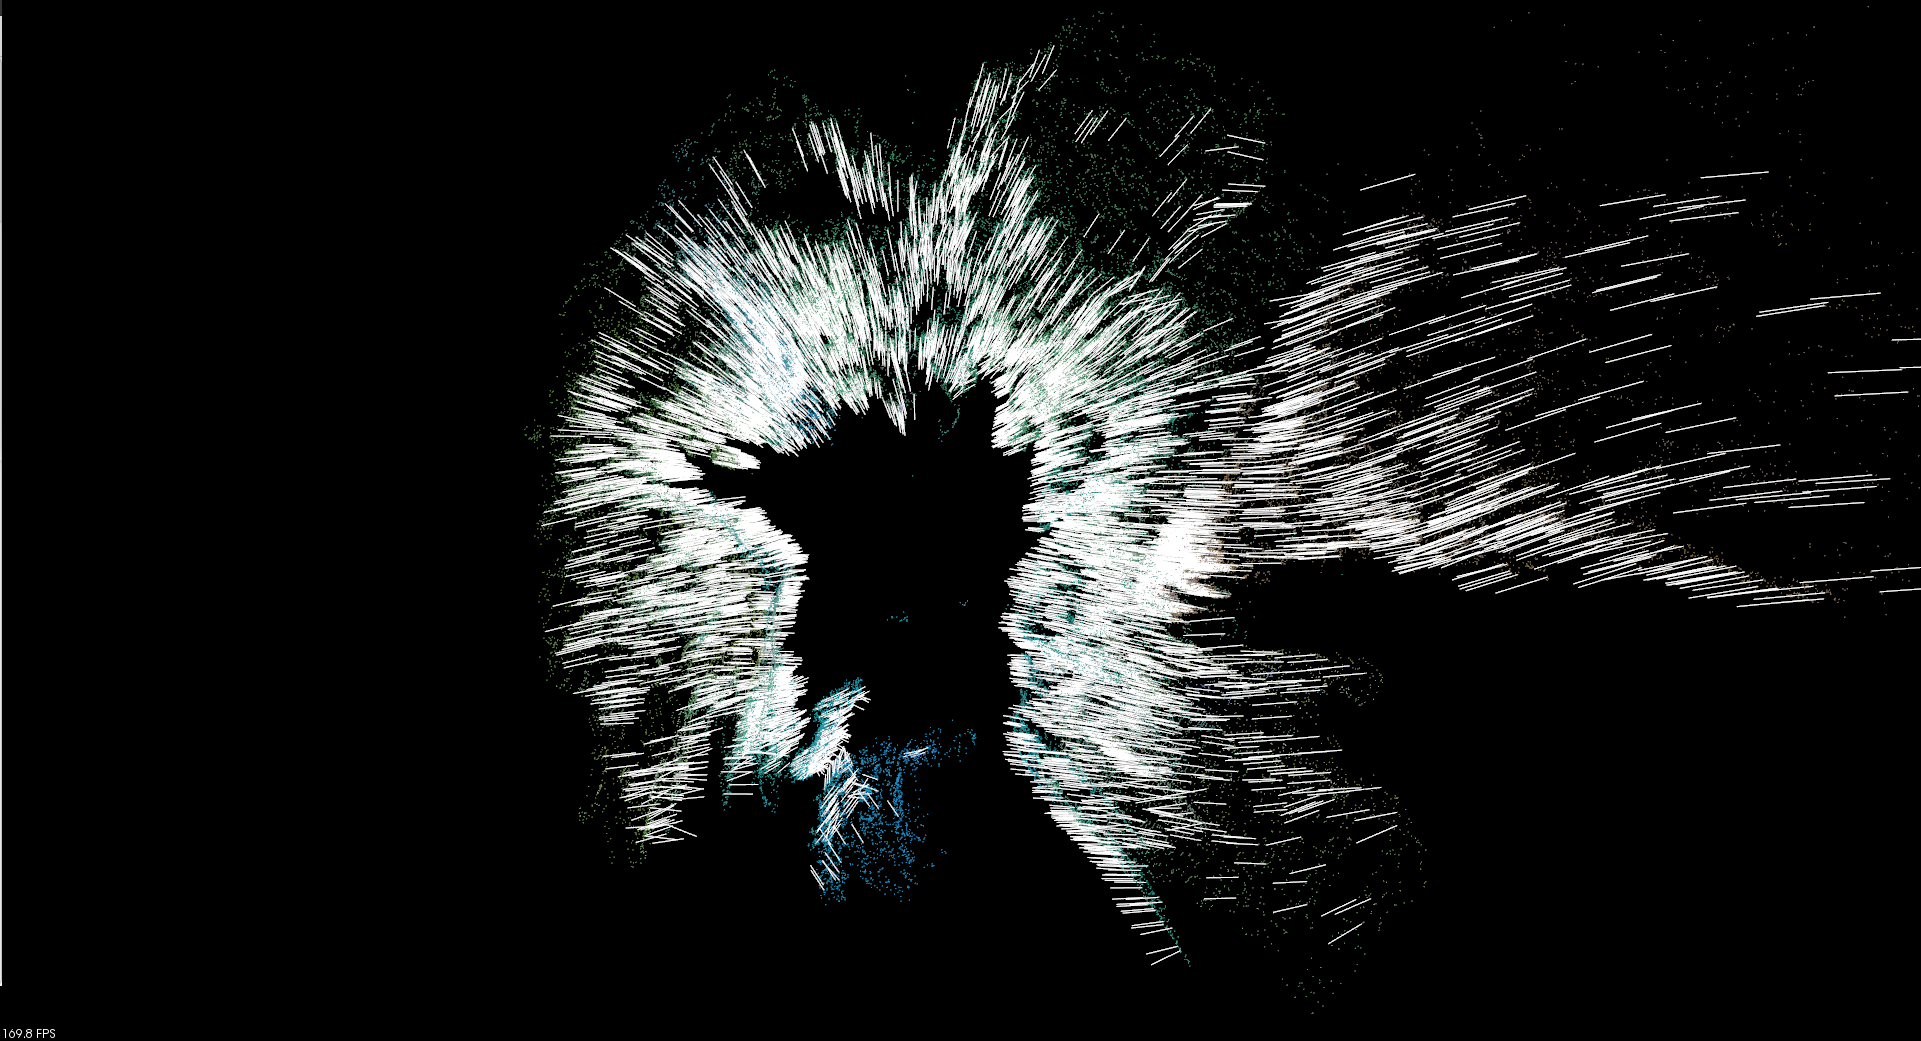
\includegraphics[width=0.95\textwidth]{./figures/normals_pcl_with}\label{fig:with_normals}}}
		\end{tabular}
		\caption{\ref{fig:without_normals} A point cloud segment of the ten second traversal. \ref{fig:with_normals} The same segment with white normal lines protruding inwards}
		\label{fig:showing_normals}
	\end{center}
\end{figure*}

Moving this normal oriented point cloud over to Meshlab allows us to now experiment with the different reconstruction techniques. These tests were run on the points generated from the first 100 frames of the ten second traversal video. Ultimately our reconstruction would never run on the full frame data set due to processing power constraints, so instead the cave would be generated in subsets and stitched together. 100 frames was enough to define the shape of the walls, and adding in more had minimal effect on the local outputs. Textures were generated using the RGB values of the input points. This looses a lot of the texture detail present in the images themselves, but a base model needed to be established first before creating a proper texture projection.  

An initial test was done using only Delaunay triangulation. This was the procedure that had been used on ocean floor mosaicking were the overall shape of the points was flatter. Unfortunately for our point cloud, Delaunay triangulation creates a completely incomprehensible mass. 

\begin{figure}[h]
	\centering
	\fbox{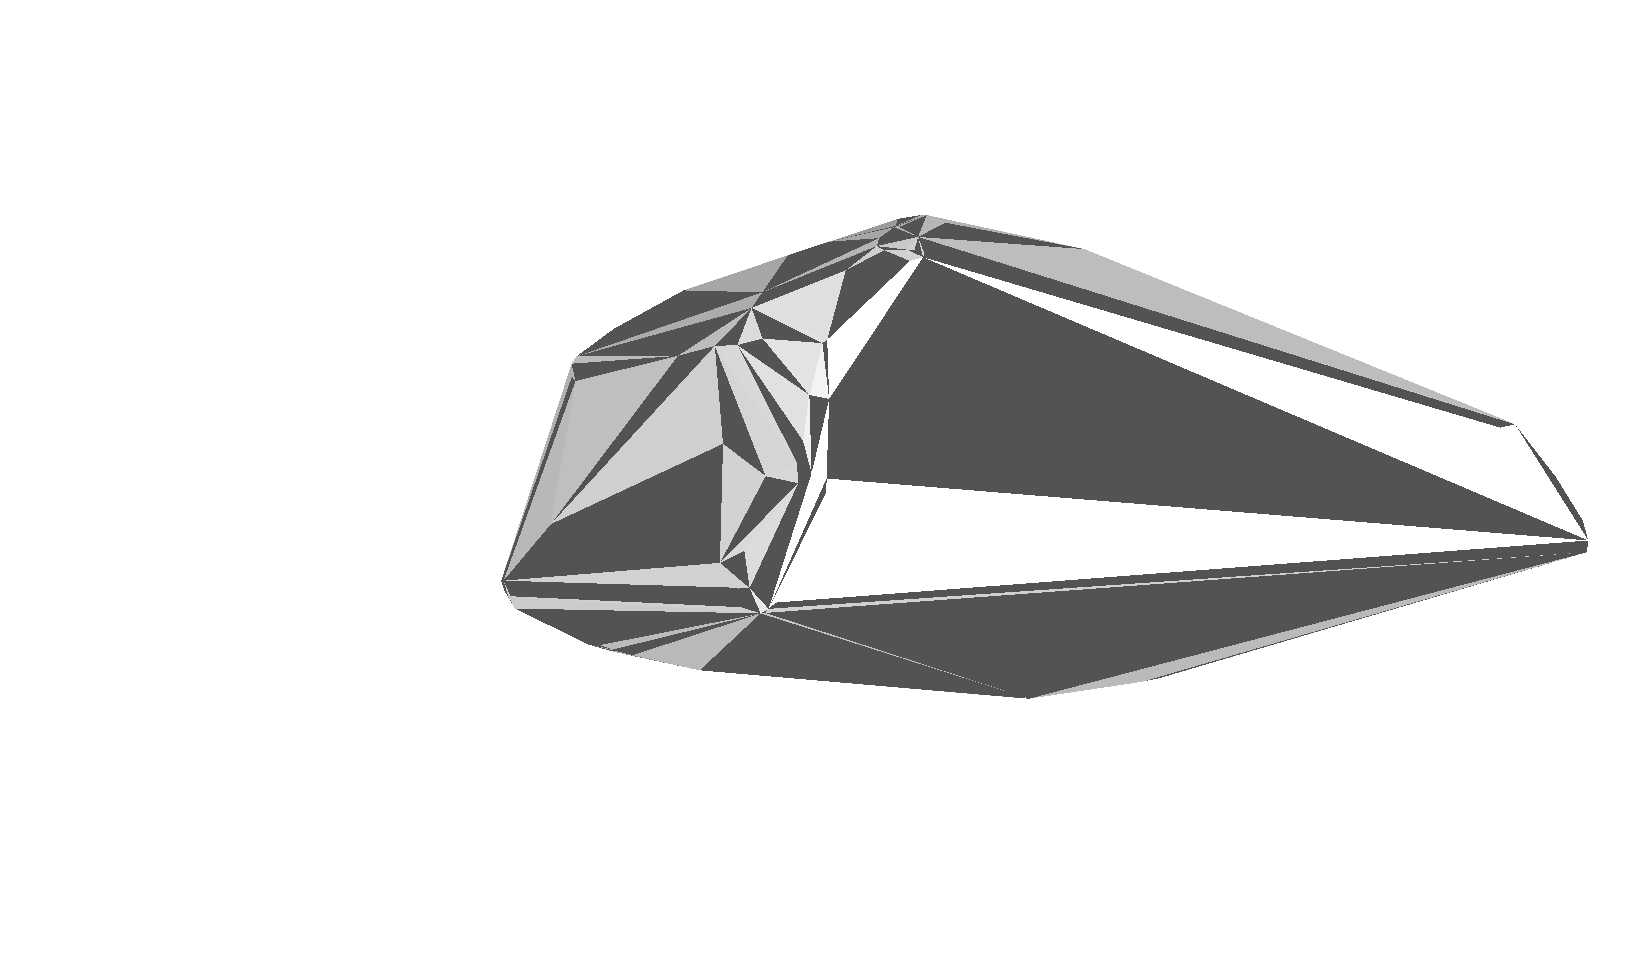
\includegraphics[width=0.95\columnwidth]{./figures/deltri01}}
	\caption{Results of running Delaunay triangulation.}
	\label{fig:deltri}
\end{figure}

\begin{figure*}[h]
	\begin{center}
		\leavevmode
		\begin{tabular}{ccc}
			\subfloat[]{\fbox{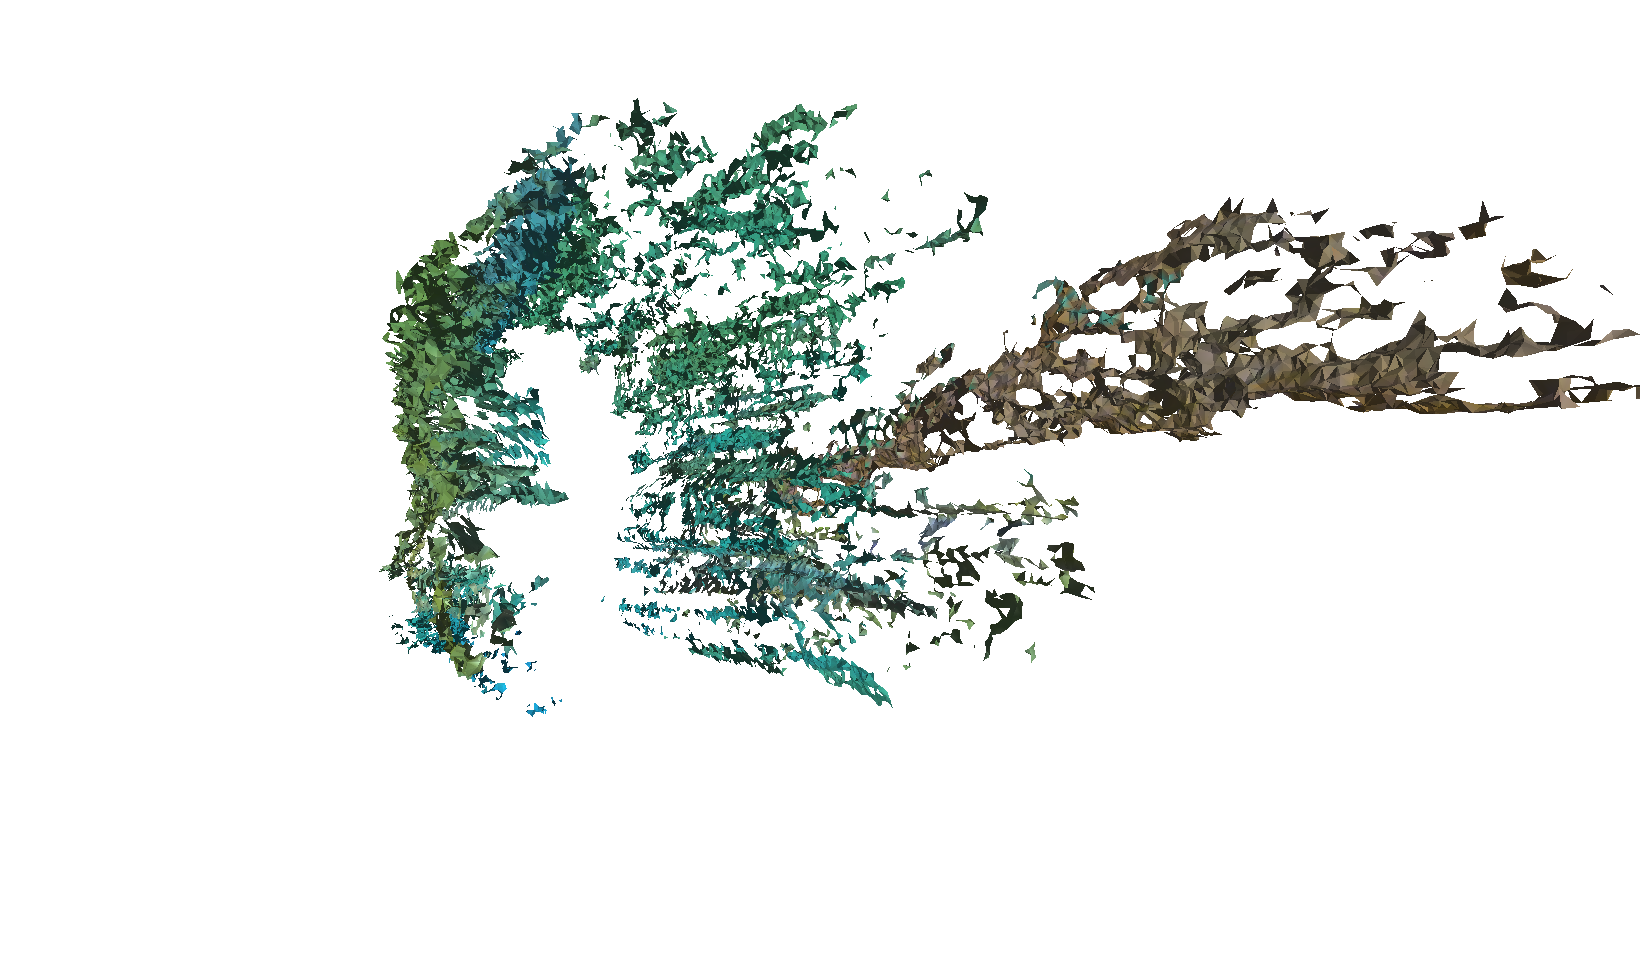
\includegraphics[width=0.55\textwidth]{figures/bp_all00}\label{fig:bp_all}}}\\
			\subfloat[]{\fbox{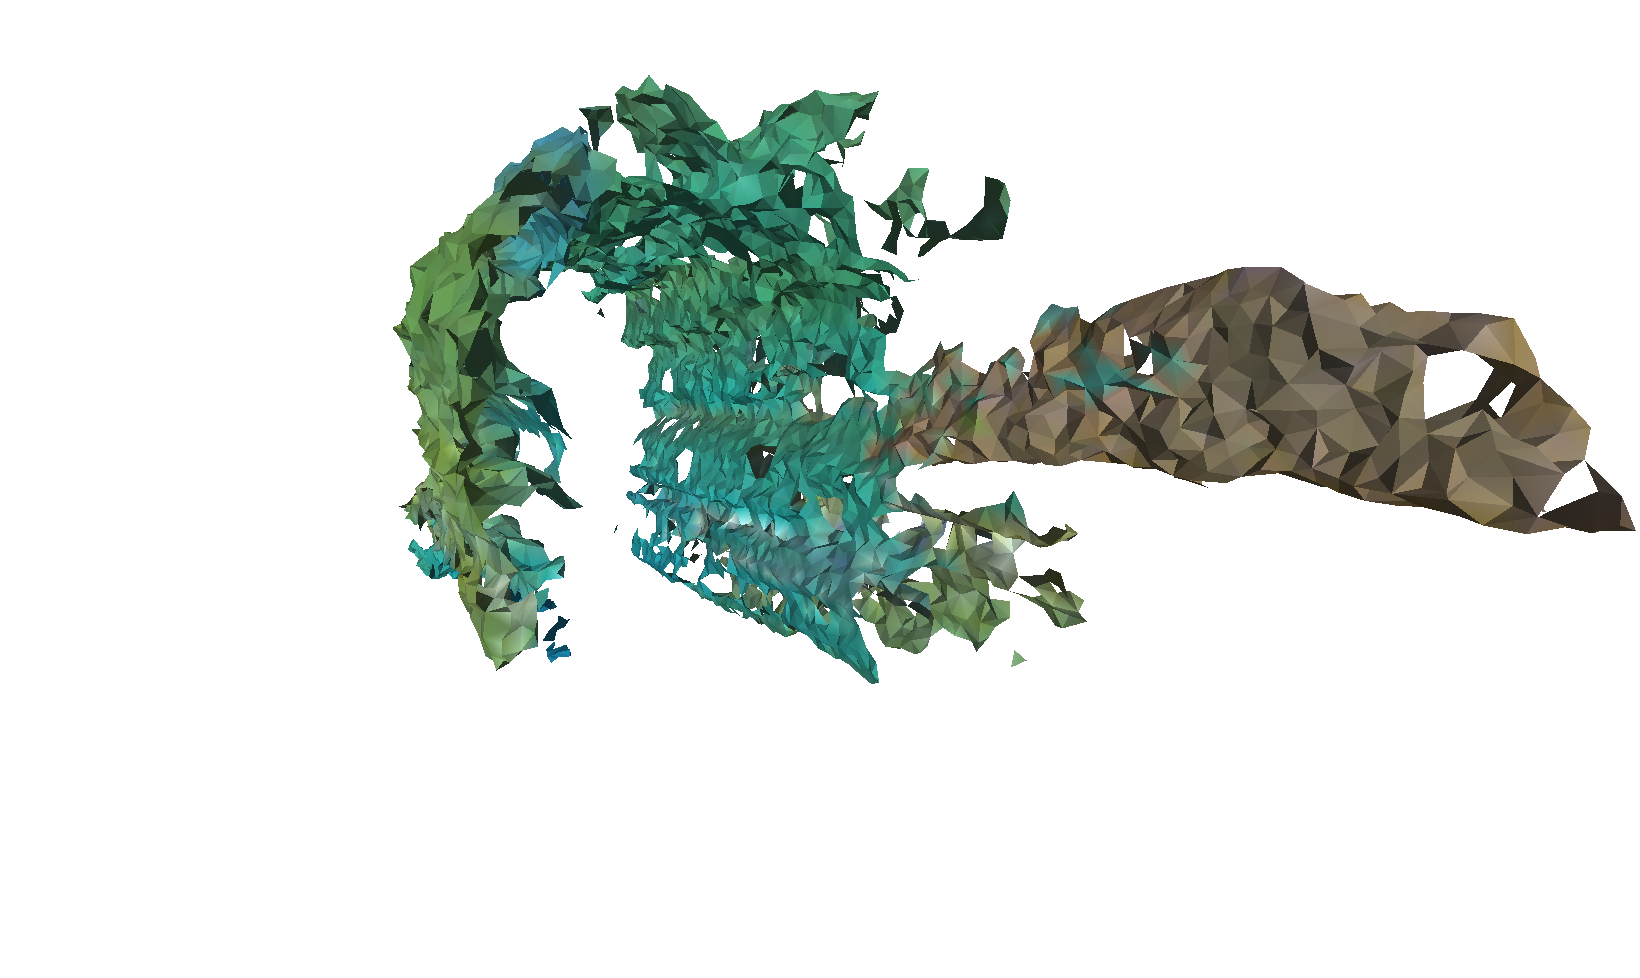
\includegraphics[width=0.55\textwidth]{figures/bp_tenthou00}\label{fig:bp_tenthou}}}\\
			\subfloat[]{\fbox{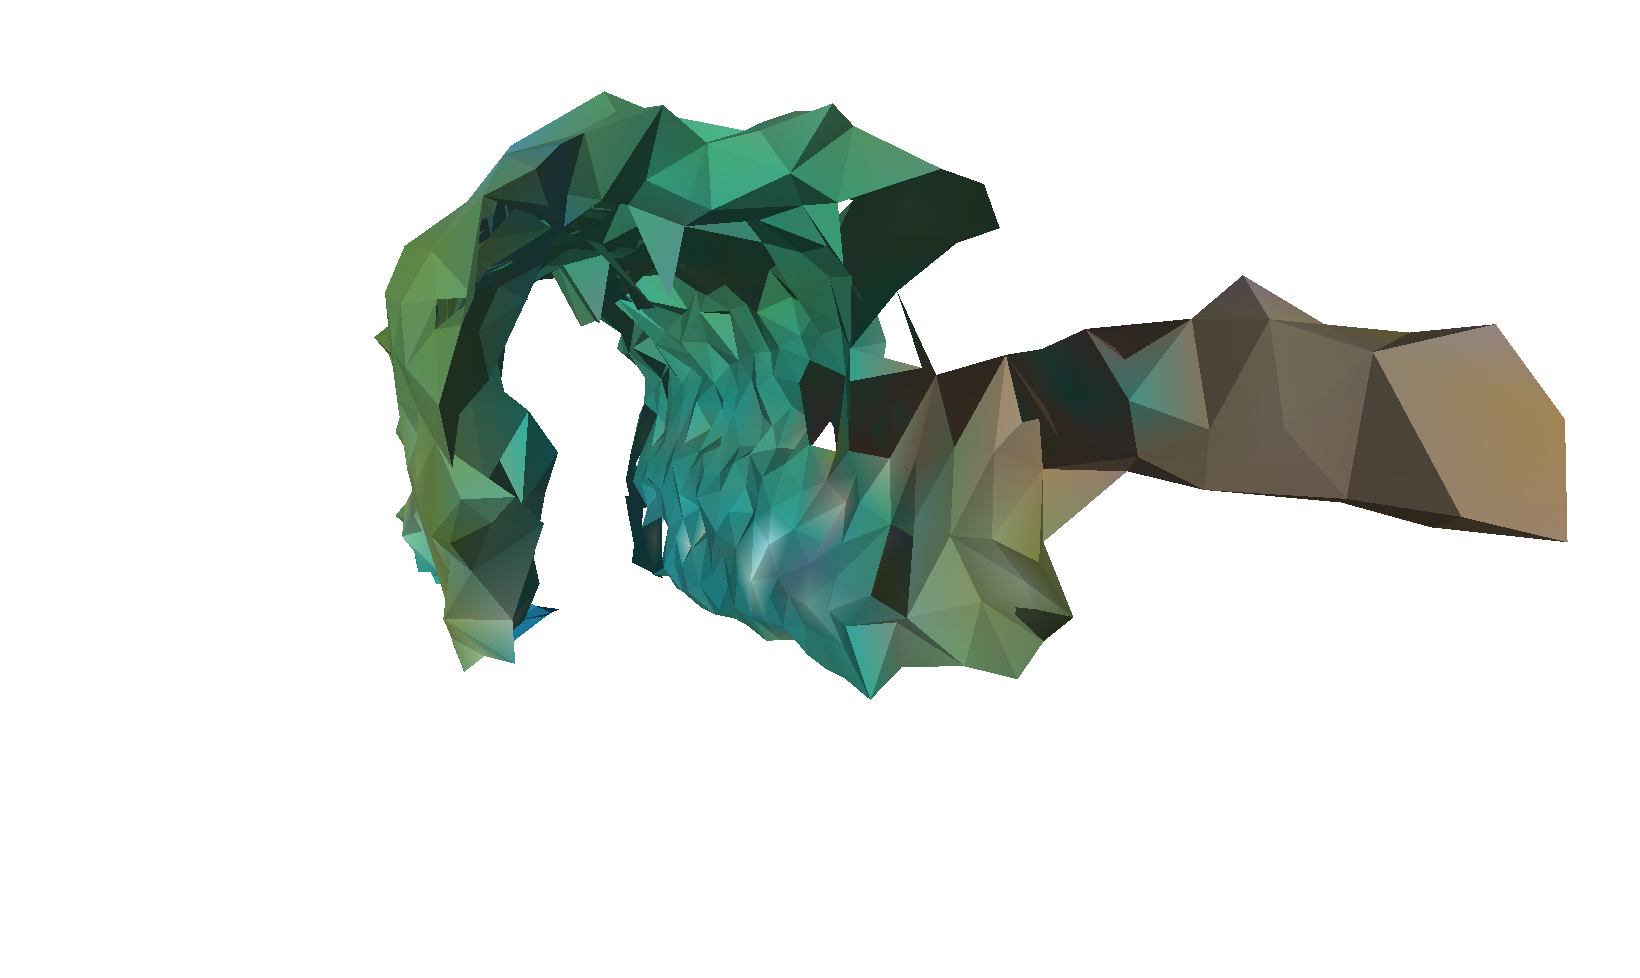
\includegraphics[width=0.55\textwidth]{figures/bp_thou01}\label{fig:bp_thou}}} 
		\end{tabular}
	\end{center}
	\caption{\ref{fig:bp_all} Ball-pivoting applied to the entire point set. \ref{fig:bp_tenthou} Applied to a 10,000 sampling. \ref{fig:bp_thou} Applied to 1,000 point sampling.}
	\label{fig:ballPivot}
\end{figure*}

If we try an interpolative method such as ball-pivoting, we see in \ref{fig:bp_all} that the results don't look much better than Delaunay triangulation. If we take sampling into account, though, dropping the total point count down from 100,000 points to 10,000 or 1,000 produces fast low res versions of the cave mesh as seen in \ref{fig:bp_tenthou} and \ref{fig:bp_thou} respectively. These can be useful in quickly generating surfaces that have at least some resemblance of the shape. 



Meshlab includes two marching-cubes based reconstruction approaches using MLS, algebraic point set surfaces (APSS)~\cite{guennebaud2007algebraic,guennebaud2008dynamic} and robust implicit MLS (RIMLS)~\cite{oztireli2009feature}. After adjusting the MLS filter scale, these methods generate the best reconstructions achieved. Both produce similar outputs, but the RIMLS method appears to create smoother surfaces in a more locations. These results are shown in \ref{fig:rimls}.

\begin{figure}[h]
	\centering
	\fbox{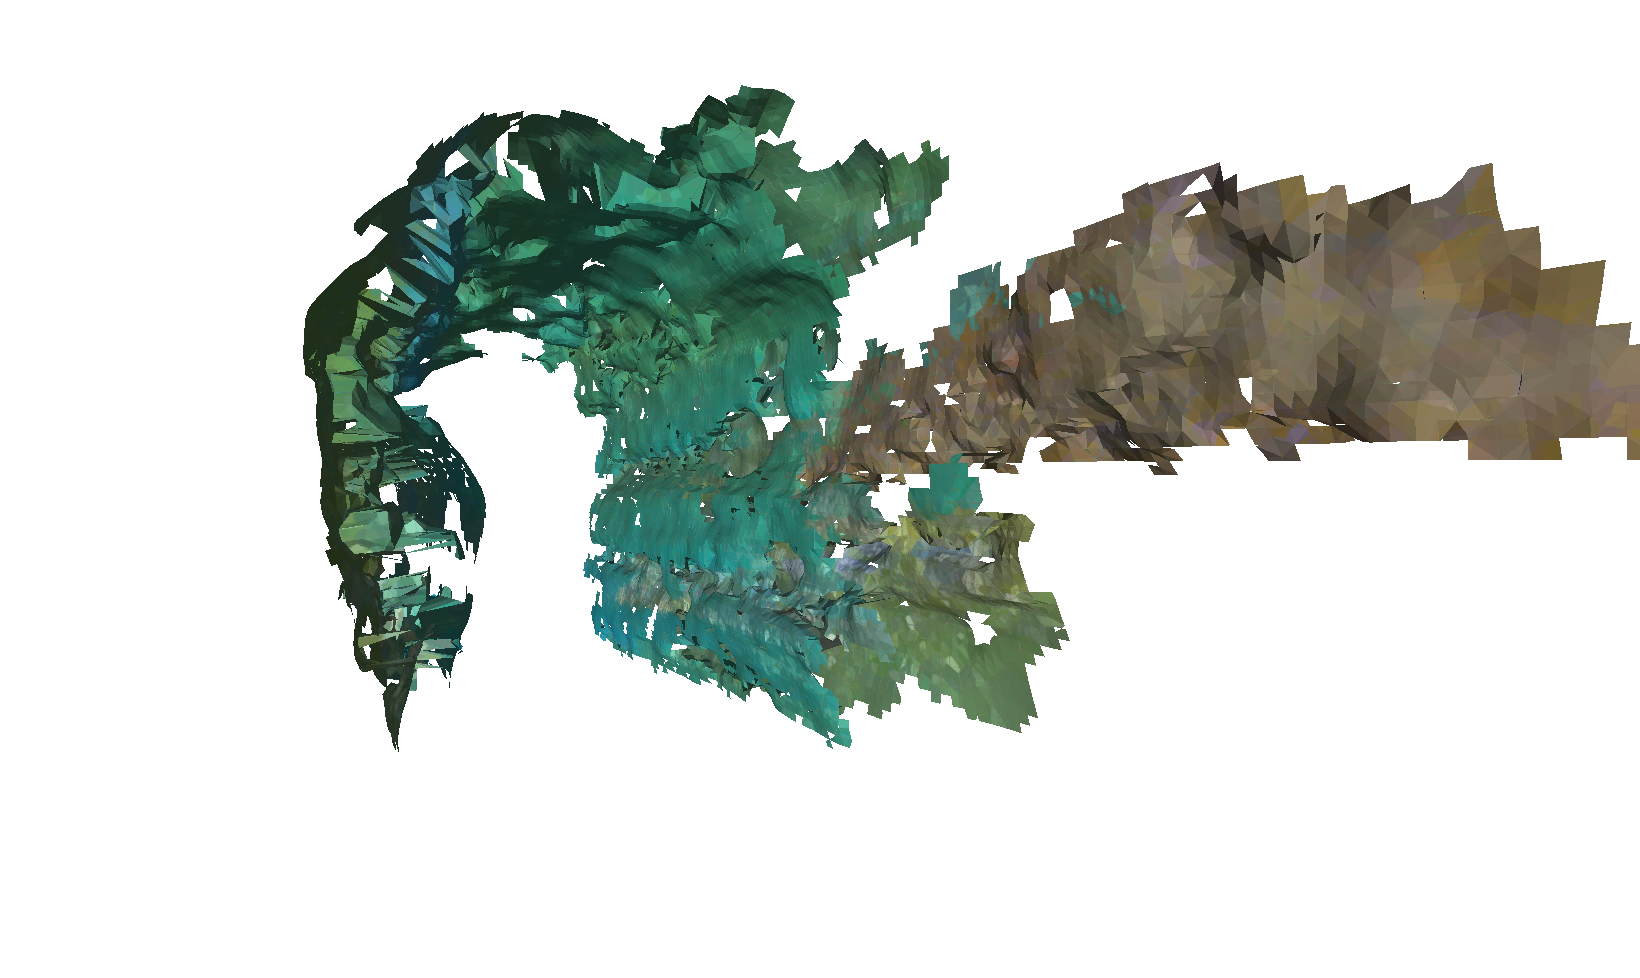
\includegraphics[width=0.95\columnwidth]{./figures/rimls00}}
	\caption{RIMLS marching cubes surface reconstruction}
	\label{fig:rimls}
\end{figure}

It is clear the shape of the cave is still not perfect. It is expected most of problems arise from our camera set up and lack of input data detail. Due to our small baseline, We loose a lot of accuracy as we move away from the camera. This is likely a cause for the misalignment occurring along the walls. These kinds of errors in our reprojection can cause reconstruction problems when points fall to closely to other points they shouldn't be near. Testing with other camera systems should shed light on areas of our reconstruction pipeline that can benefit from finer tuning. 

%\include{Squares}         %% The three sections of Chapter 1 
%\input{Cube}             %% are in the files Squares.tex,  
%\input{Hypercubes}	   %% Cubes.tex and Hypercubes.tex
       
                           
%\include{1mod4}
%\input{flying}
%\input{joins}
%\input{wattage}

%\include{3mod4}	          %% This chapter has 8 sections
%\input{bigtime}         %% You should give your sections
%\input{smalltime}       %% logical names, rather than
%\input{roadmap}         %% numbers. As you write, you might
%\input{overview}        %% decide to rearrange things. 
%\input{turnabout}       %% LaTeX can keep track of the
%\input{fairplay}        %% numbering for you.
%\input{roundup}

%\include{rest}
%\input{relax}
%\input{grin}


\chapter*{Conclusion}
\addcontentsline{toc}{chapter}{Conclusion}
This thesis presented contributions to the topics of camera calibration, stereo shape estimation, and surface reconstruction for the application of reconstructing 3\hyp D models of underwater cave systems. In order to help calibrate camera systems with extreme distortion such as the GoPro in SuperView mode, we studied calibration techniques that took into account the removal of outlier images. MATLAB's computer vision system toolbox was found the be the most effective way to handle the problems of high distortion systems, and a simplified OpenCV version of their outlier removal was ported over. With a successfully calibrated camera we presented the first ever reconstruction results from an underwater cave using a novel approach utilizing the artificial lighting of the scene as a tool to map the boundaries. This approach was applied on actual collected cave dive footage, and was effective in both producing a reconstruction and not interfering with the standard procedure the cave divers follow. Lastly the point cloud underwent a series of tests for surface reconstruction using a number of the most prominent techniques in the field.

We identified a number of areas for which future work can expand upon through the study of our tests and results. Different camera systems with a larger baseline and even more reduced calibration error will hopefully create more accurate reconstructions that in turn lead to more accurate surfaces. The inclusion of additional non obtrusive sensors such as sonar can also increase the accuracy of our results. 

Cave mapping is a problem with significant impact across a wide range of fields. Steps made towards increasing the accuracy and efficiency of these mappings, especially at a low cost and non-cumbersome level, is vital. This work introduces a pivotal first step towards achieving complete mappings..      %% Honors theses are required to 
                          %% have an unnumbered chapter
                          %% for conclusions.  The file
                          %% Conclusion.tex should begin
                          %%   
                          %% \chapter*{Conclusion}
                          %% followed by the appropriate
                          %% text.


\printbibliography %%  This is the command to use to
			       %%  insert the bibliography if you are using
                           %% the biblatex.sty package.  See the 
                           %% uscthesisdoc.pdf documentation for
                           %% for alternative bibliographic systems.     

\Appendix                 %% Use this command if you have one 
                          %% appendix. Use \Appendices if you 
                          %% have more than one.
	
\chapter{OpenCV Port}
%\section{OpenCV Port}
While the MATLAB Computer Vision system Toolbox is highly powerful and produced good results for our setup, there are drawbacks. Namely MATLAB is closed source software that requires payment to use. At the same time, MATLAB can be tedious to integrate with external applications and thus might not be ideal if camera calibration is only a part of a larger pipeline. OpenCV on the other hand is both widely used for a variety of image and computer visions applications, and is both open source and easy integrate. As noted earlier, OpenCV has implementations of camera calibration already and they are simple to use. Unfortunately they lack the user interface and built in outlier removal to make calibrating something like SuperView efficient. A similar implementation of the MATLAB outlier removal system was thus developed as an easy to use tool in OpenCV.

Because data visualization plays such a crucial role in identifying bad calibration input images, there needed to be a good way to generate interactive graphs of the OpenCV calibration results. This can be time consuming in C++, so alternatively python's Matplotlib library was used to recreate as similar output as possible to MATLAB's. OpenCV has both a C++ and a python library, but python was found to quite slow in calibrating large data sets. Due to this, a hybrid C++ and python application was created. The finalized control flow is as follows. 

\begin{enumerate}
	\item The C++ application reads in a set of input image pairs for calibration
	\item The calibration board corner points are detected and stored in an external file
	\item The first calibration run takes place and the reprojection error of every input image is stored in an external file along with the average reprojection error
	\item A python script reads the reprojection errors and plots them along with an average reprojection error line
	\item The user adjusts the average reprojection error line, selects outlier removal button, and the file of corner points is edited down to the new smaller set
	\item The C++ application reads in the corner points, avoiding time spent calculating the corner points again, and recalculates the reprojection errors with the new set
	\item The output is again used in the python script and the process is repeated
\end{enumerate}

Fig. \ref{fig:cvrepro} shows the plot generated by the OpenCV port, and the reprojection error for the image set of \ref{fig:results1}. After iterative outlier removals, the error is brought down from the original 2.83 to 1.02. This compares to MATLAB's error output of .51. Because MATLAB is a closed source application, the exact method for calibration can not be ported over directly. This means MATLAB's calibration probably involves a slightly refined calculation and optimization. OpenCV has trouble matching MATLAB's results and its speed, but compared, but this method still provides an open source alternative. These results match or are even better than hand picking input images and saves time eliminating bad options. 

\begin{figure}[th]
	\centering
	\fbox{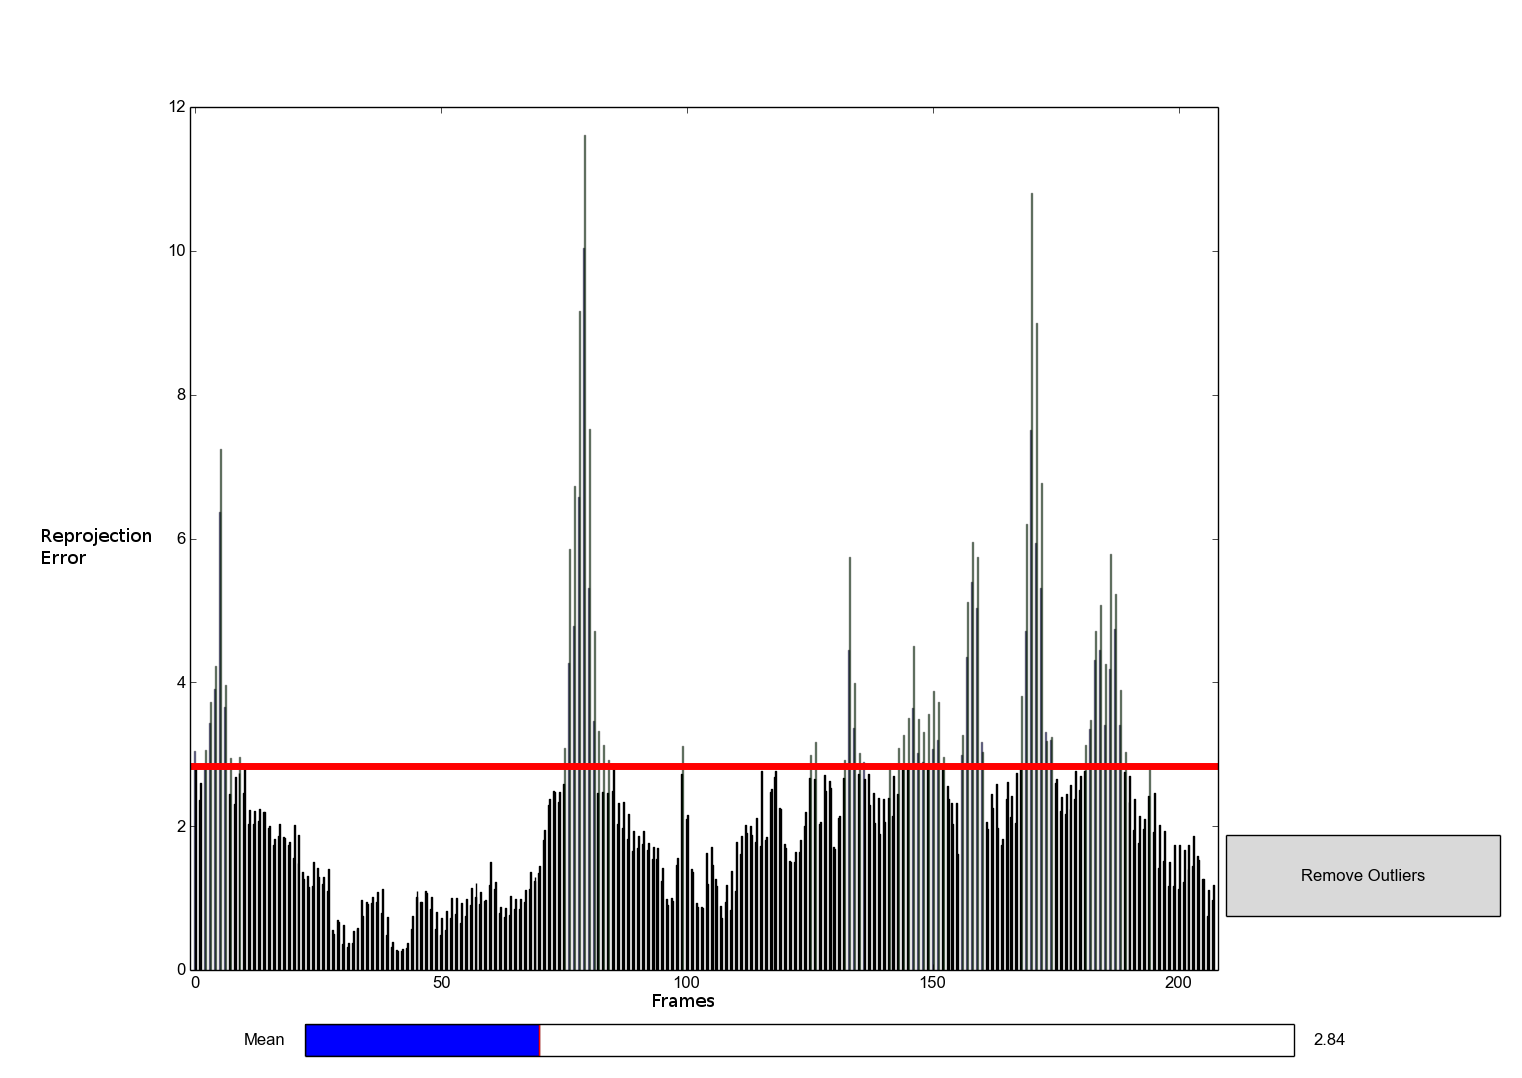
\includegraphics[width=0.95\textwidth]{./figures/allframes_axes_labels}}
	\caption{Initial reprojection errors plotted in python}
	\label{fig:cvrepro}
\end{figure}
%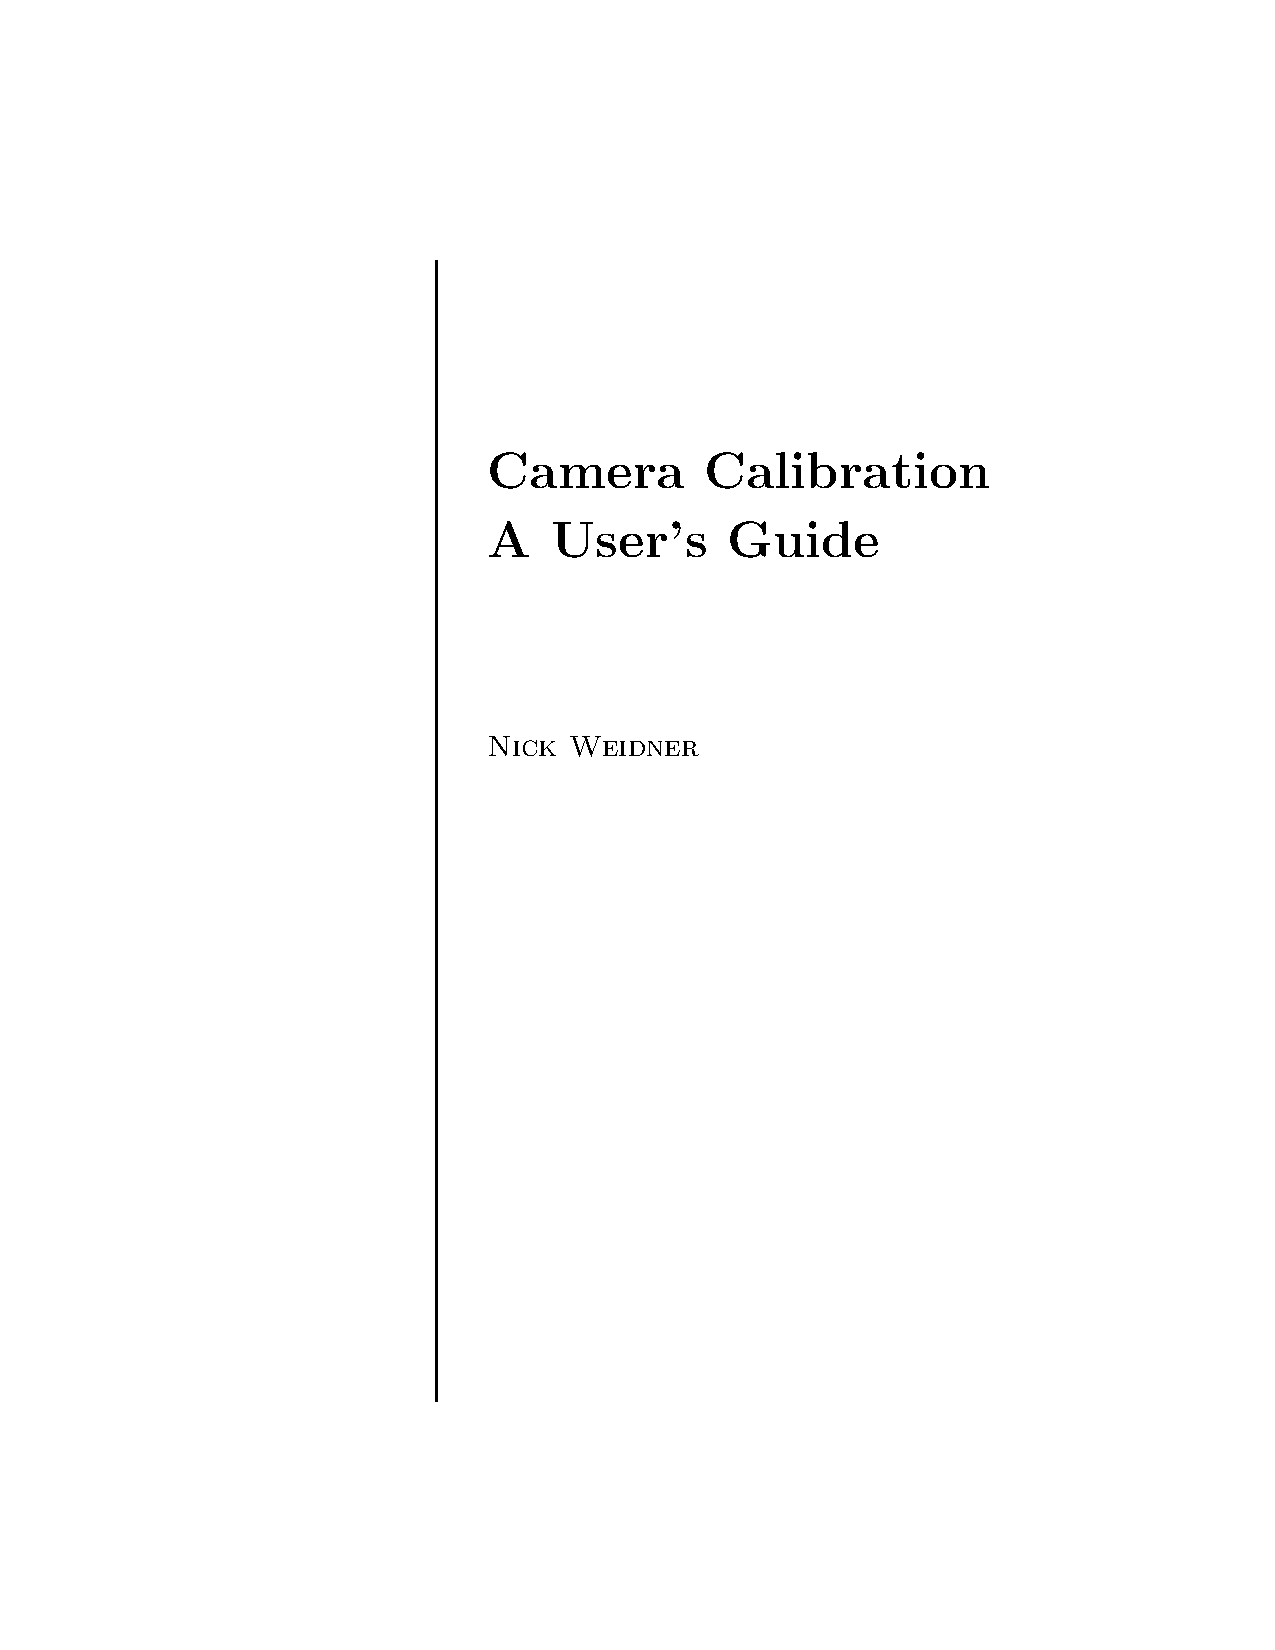
\includepdf[pages={1-},pagecommand=\thispagestyle{plain}]{weidner_CalibrationGuide.pdf}
%\documentclass{article}

\usepackage[utf8]{inputenc}
\usepackage[english]{babel}
\usepackage[english]{isodate}
\usepackage[parfill]{parskip}
\usepackage{graphicx}
\usepackage{amsmath}
\usepackage{listings}
\usepackage[hidelinks]{hyperref}
\usepackage{fixltx2e}
\usepackage{listings}

\setcounter{tocdepth}{4}
\setcounter{secnumdepth}{4}

\setlength\parindent{24pt}

\title{Camera Calibration}
\author{Nick Weidner}

\newcommand*{\titleGM}{\begingroup % Create the command for including the title page in the document
	\hbox{ % Horizontal box
		\hspace*{0.2\textwidth} % Whitespace to the left of the title page
		\rule{1pt}{\textheight} % Vertical line
		\hspace*{0.05\textwidth} % Whitespace between the vertical line and title page text
		\parbox[b]{0.75\textwidth}{ % Paragraph box which restricts text to less than the width of the page
			
			{\noindent\Huge\bfseries Camera Calibration \\[0.5\baselineskip] A User's Guide}\\[2\baselineskip] % Title
			{\large \textit{}}\\[4\baselineskip] % Tagline or further description
			{\Large \textsc{Nick Weidner}} % Author name
			
			\vspace{0.5\textheight} % Whitespace between the title block and the publisher
			{\noindent  \plogo}\\[\baselineskip] % Publisher and logo
}}
\endgroup}

\begin{document}
\pagestyle{empty}
\titleGM
\iffalse
\begin{titlepage}
	\vspace*{\stretch{1.0}}
	\begin{center}
		\Large\textbf{Camera Calibration, User's Guide}\\
		\large\textit{Nick Weidner}
	\end{center}
	\vspace*{\stretch{2.0}}
\end{titlepage}
\fi
	
\pagenumbering{Roman}
\tableofcontents
\newpage
\listoffigures
\newpage
\pagenumbering{arabic}

\section{Preface}

Camera Calibration is the backbone, and often first step in any project involving imaging from a camera. Images that are not corrected to account for camera parameters that cause distortion and misalignment are incorrect 2D mappings af the physical world. This means any spatial calculations made with these raw images will inaccurate. When correcting these images, it is practically impossible to accurately calculate a correction with zero error in the pixel values. Any error present can thus compound with all the later error accumulated from future calculations. This is why camera calibration is such a vital first step when working with images. While it may be considered by many to be a long and solved problem, no two data sets are one hundred percent alike. It is important to calibrate carefully, minimize error, and not take the process for granted unless ensue headaches down the road. 

This user's guide is structured to give anyone an overview of the tools out there, and approaches to use to get the best results when calibrating a camera. The two primary packages recommended here are OpenCV and the Matlab Computer Vision System Toolbox. There are a few other Matlab packages and other standard coding library packages out there that can do camera calibration, but they all work similarly on a fundamental level and this guide will address why these are highlighted and when to use which one. It is highly recommended to look over the underlying theory of camera calibration addressed in this guide as well. Many obstacles such as input and output problems can be easily resolved if one understand what goes on behind the scenes and avoids simply calling library functions and expecting an output. 

\section{Underlying Theory}

There are numerous resources on camera calibration in books, in papers, and across the web. A general overview is given here.

\subsection{Pinhole Camera}

We calibrate a camera to identify data on it's most important components. Important for image work at least. These components are...

\begin{itemize}
	\item Focal Length
	\begin{itemize}
		\item The distance from the center of a lens to the focus in the camera
	\end{itemize}
	\item Principal Point
	\begin{itemize}
		\item The location on the image from which the perspective is centered, usually the center of the image.
	\end{itemize}
	\item Distortion 
	\begin{itemize}
		\item How the image changes when it is projected through a lens
	\end{itemize}
	\item Base Line (in stereo systems)
	\begin{itemize}
		\item The distance between the focus of the left and right camera
	\end{itemize}
\end{itemize}
	
If we simplify our system to a pinhole camera model with no lens, then the 3D world maps to a 2D one like this. 

\begin{figure}[h]
	\centering
	\fbox{\includegraphics{./figures/camera_calibration_focal_point.png}}
	\caption{Pinhole camera model}
	\label{fig:pinhole}
\end{figure}

The model itself is mathematically represented as...

\[
sm' = A[R|t]M'
\]

or

\[ s 
\left[\begin{array}{c} u \\ v \\ 1 \end{array} \right]
=
\begin{bmatrix}
f_x & 0 & c_x \\ 0 & f_y & c_y \\ 0 & 0 & 1
\end{bmatrix}
\begin{bmatrix}
r_{11} & r_{12} & r_{13} & t_1 \\ r_{21} & r_{22} & r_{23} & t_2 \\ r_{31} & r_{32} & r_{33} & t_3
\end{bmatrix}
\left[\begin{array}{c} X \\ Y \\ Z \\ 1 \end{array} \right]
 \]
 
where:

\begin{itemize}
	\item (X,Y,Z) are coordinates of a 3D point in the world
	\item (u,v) are the coordinates of the same point projected as a pixel on the image
	\item (cx,cy) are the principal point coordinates
	\item fx, fy are the focal lengths in pixel units
\end{itemize}

The A matrix is often regarded as the camera matrix or a matrix of intrinsic parameters. These are the parameters within the camera itself. The \lstinline![R|t]! matrix is a matrix of extrinsic parameters and is used to describe the camera motion around a static scene in regards to rotation and translation. \lstinline![R|t]! translates coordinates of a point in (X,Y,Z) to a coordinate system that is fixed with respect to the camera. 

Using this simple model, a 3D coordinateat (X,Y,Z) can be represented as pixel coordinates u,v as...

\begin{align*}
u&=f_x \times \frac{X}{Z} + c_x & v&=f_y \times \frac{Y}{Z} + c_y
\end{align*}

\subsection{Distortion}

No modern day camera is as simplistic as a pinhole model, and the lens used introduces a wide variety of distortions. The most common forms of distortion arise from radial and tangential distortion. Radial distortion the distortion of light through the lens that causes the image to change it's shape. Tangential distortion is the distortion that arises when a cameras parts are not manufactured directly in line with each other, and the lens and sensor are not completely parallel. Tangential distortion is often minimal, but still worth taking into account. Radial distortion is often much more dramatic, and almost all cameras use a different enough lens that no two cameras have an identical mapping. 

Radial primarily shows up in these forms...

\begin{figure}[h]
	\centering
	\fbox{\includegraphics{./figures/calibration_radial_distortion.png}}
	\caption{Radial Distortion}
	\label{fig:radial}
\end{figure}

Barrel and pincushion distortion are mathematically quadratic and can be described by a quadratic polynomial. Depending on the exact shape of a physical lens,  quadratic system may not fit the shape exactly and a higher degree even polynomial fits better. Note an odd degree polynomial would not fit the shape of a lense.  Most practical lenses don't follow a degree higher than 6 because the distortion at a higher degree becomes so minimal. 

These distortions alter our pinhole model to...

\begin{align*}
x'&= X/Z & y'&= Y/Z & r^2 &= x'^2 + y'^2
\end{align*}

\[
x'' = x' \frac{1+k_1r^2+k_2r^4+k_3r^6}{1+k_4r^2+k_5r^4+k_6r^6} + 2p_1x'y' + p_2(r^2 + 2x'^2)
\]

\[
y'' = y' \frac{1+k_1r^2+k_2r^4+k_3r^6}{1+k_4r^2+k_5r^4+k_6r^6} + p_1(r^2+2y'^2) + 2p_2x'y'
\]

\begin{align*}
u &= f_x \times x'' + c_x & v&=f_y \times y'' + c_y
\end{align*}

Where k\textsubscript{1},k\textsubscript{2},... are the radial distortion values and p\textsubscript{1} and p\textsubscript{2} are the tangential distortion values. The equation shown above is specifically the underlying model for OpenCV camera calibration depending on whether the user wants 2, 3, or all 6 coefficients calculated. It is worth noting that the Matlab computer vision system toolbox uses the same model, but only uses 2 to 3 radial coefficients depending on the severity of the distortion. Both are based on the widely famous Brown-Conrady model for which takes in n radial distortion coefficients. 

An alternative distortion model has also been introduced in OpenCV called the fisheye camera model. This model alters the pinhole model to...

\begin{align*}
x'&= X/Z & y'&= Y/Z & r^2 &= x'^2 + y'^2 & \theta &= atan(r)
\end{align*}

\[
\theta_d = \theta(1+k_1\theta^2+k_2\theta^4+k_3\theta^6+k_4\theta^8)
\]

\begin{align*}
x'' &= \frac{\theta_d}{r} \times X & y'' &= \frac{\theta_d}{r} \times Y
\end{align*}

\begin{align*}
u &= f_x \times x'' + c_x & v&=f_y \times y'' + c_y
\end{align*}

This model lacks descriptive documentation of its behind the scenes in OpenCV, but it is based on a more generic camera model and calibration method for wide angle lenses. This has also been  implemented in another Matlab calibration package called the Camera Calibration Toolbox for Matlab.

\subsection{Calibration}

These models are great for transforming world points when we know all of the values, but the whole point of calibrating a camera is that we don't know what any of these values are. This is where the packages come into play. The functions in these packages are designed to take in points from the world and solve a curve fitting problem in order to identify the parameters that most accurately project a point. If not careful, curve fitting problems can inaccurately return solve for a local minimum. This means that parameters can be found that fit our data really well, but work horribly on additional data sets. This makes choosing the data sets very important and will be addressed more in depth later on. In the end, the values we return as our best fit for our data, are going to give off pixel error. This error states how many pixels off from where it should be a pixel is when run through our model. 

\subsection{Stereo}

When introducing another camera into the mix there are a few additional things to consider and calculate. The individual calibration still needs to be done and this is still done independently, nothing in this process is effected by the other camera. Once calibrated, though, the cameras need to be rectified, which means they need to be aligned either horizontally or vertically depending on their orientation. This creates a new camera matrix following the form...
	
\begin{align*}
C1 &=
\begin{bmatrix}
f_x & 0 & c_{x1} & 0\\ 0 & f_y & c_y & 0\\ 0 & 0 & 1 & 0
\end{bmatrix} &
C2 &=
\begin{bmatrix}
f_x & 0 & c_{x2} & T_x \times f\\ 0 & f_y & c_y & 0 \\ 0 & 0 & 1 & 0
\end{bmatrix}
\end{align*}

This is for the case of horizontal stereo and T\textsubscript{x} represents a horizontal shift in the cameras.This is important for calculating a disparity map which identifies the spacial differences of each pixel between the left and right image. 

\section{Getting Started}

Before starting camera calibration, a few things need to be set up and the proper tool for the job needs to be decided on. 

\subsection{Picking the Proper Tool}

In most cases, the basic OpenCV camera calibration functions will easily get the job done. Most cameras calibrate through a very straightforward pipeline and return good results. This is a good place to start if you are unsure. Calibration gets tricky when there is a significant amount of distortion in the camera lens. A fisheye or wide angle lens can sometimes return large error values on the standard OpenCV calibration functions. The OpenCV fisheye calibration functions work nicely here.

 Sometimes the distortion is so dramatic, though, OpenCV struggles to minimize the error. At least not without an exceedingly long and tedious testing process from the user. This is where Matlab shines. The Matlab computer vision system toolbox calibration tool has a built in error plot that helps you identify bad input images. There is no tool for OpenCV directly, so all images must be hand picked. This is usually fairly straight forward, but not on extremely distorted images. 
 
 The GoPro superview camera mode is an example of where Matlab is able to minimze the error, but not OpenCV. If using a GoPro camera make sure to check what mode the recording is done in. Superview is the default on some models, yet it serves practically no purpose when calibration needs to be done because the edges are eventually cropped down to the non superview size anyway and error is much better without it. Here is a short pro and con list of OpenCV vs Matlab.  

\begin{align*}
\begin{tabular}{r|p{0.4\textwidth}}
	OpenCV \\
	Pros & \begin{itemize}
		\item Open source
		\item Very configurable to needs of project
		\item Output is readily available and coincides with other Opencv functions 
		\item Both the standard and fisheye models operate in similar manners 
	\end{itemize} \\
	Cons & \begin{itemize}
		\item Input of images can be tedious
		\item Debugging can be more complicated 
		\item Configurability can make simple things overly confusing
		\item Fails on extremely distorted image sets like the GoPro superview
	\end{itemize}
\end{tabular}
\begin{tabular}{r|p{0.4\textwidth}}
	Matlab \\
	Pros & \begin{itemize}
		\item Easy to set up and use
		\item Easy to combine with other matlab functions 
		\item Error plotting tool makes image selection less tedious
		\item Has success on more distorted image sets like the GoPro superview
	\end{itemize} \\
	Cons & \begin{itemize}
		\item Requires a Matlab license and a package license for the tool
		\item Output data is tedious to use outside of Matlab
		\item Undistortion must be done in Matlab as well
	\end{itemize}
\end{tabular}
\end{align*}

Keep in mind what you intend to do with your data after the camera has been calibrated. If Matlab has all the functionality for what you are trying to do, it is probably easier to do everything in it. If you intend to use OpenCV later down the road, getting the proper results can be tedious from Matlab. For example, undistorted images can be produced with the undistorted parameters at any time once calculated. Matlab undistorts the images differently so any new image set using Matlab calibration parameters has to be run through matlab. There may be a way to do this properly in OpenCV, but none that I could find. 

\subsection{Setting Up}

To start using the Matlab tool, all that is required is Matlab version R2013b or later, and the Computer Vision System Toolbox. The full documentation for the tool can be found at \url{http://www.mathworks.com/help/vision/index.html}

For OpenCV, OpenCV 2.4 or 3.1 should be downloaded from \url{http://opencv.org/downloads.html}. This guide was written with OpenCV 3.1 in mind. I recommend having multiple installs on your machine in case anything comes up that is version specific. You should also download cmake from \url{https://cmake.org/} and create a CMakeList.txt like the following for your project.


\begin{lstlisting}[language=python, frame=single]
cmake_minimum_required(VERSION 3.1)
project( DisplayImage )
find_package( OpenCV REQUIRED )
add_executable( calibration calibration.cpp )
target_link_libraries( calibration ${OpenCV_LIBS} )
\end{lstlisting}

Some may prefer using python with OpenCV which has all of the camera calibration functions available as well. Python is much easier to get up and running quickly and the logical flow of the C++ code is the same. Keep in mind that when using the fisheye model, some of the python functions I found broken. 

The input for camera calibration can be either video or a series of images. Calibration works on a frame by frame basis so they is not much difference. There is a slight distinction, though. When reading video you either need to process every frame or a subset of frames across a common interval. This does not guarantee the optimal selection of input images, so it is recommended to separate videos out frame by frame and compile a set of input images. Matlab requires you to do this as there is no read video option in the toolbox. 

\section{Calibration Input}

Most of the making of breaking of good camera calibration comes from the input parameters. This section will look at how to choose good data, and common errors to avoid when doing so. 

\subsection{Brief Overview}

As mentioned before, calibration algorithms work by curve fitting and equation based on a set of input data. This input data is collected using a camera calibration board. 

\begin{figure}[h]
	\centering
	\fbox{\includegraphics[width=0.45\textwidth]{./figures/checkerboard_7x6_50x50cm-1.png}}
	\caption{7x6 Calibration Board}
	\label{fig:board}
\end{figure}

Using corner detection functions built into OpenCV and Matlab, we can identify the pixel coordinates of board corners on an image taken with a printed one. Taking images when the board is positioned at different distances, positions, and orientations, these corner points provide input for which coefficients can be fit to. 

\subsection{Picking Images}

To avoid the problem of local minimum that was discussed earlier, a wide range of board orientations should be used as input images. Calibration will work on a single image, but for any other images the undistorted will be horribly wrong. A good choice of input images are ones that cover the entirety of the image plane at a range of distances and orientations. This is an example of a low error image set I used to calibrate our underwater stereo rig cameras. 

\begin{figure}[h]
	\centering
	\fbox{\includegraphics[width=1\textwidth]{./figures/combine_images_final.jpg}}
	\caption{Mosaic of Good input images used}
	\label{fig:cornerselect}
\end{figure}

The most valuable ranges are the very close up and medium distance ranges since they cover the most image space. Ideally, try and get images of the board flat in the center, edges, and corners, and angled a few ways in the center, edges and corners both both distance ranges. You can also get a few at a farther distance. Ideally check the error you are getting with your image set and adjust accordingly. Preferred pixel error is less than 0.5. Anything larger than 1 should be examined for missing image coverage positions and anything larger than 5 probably needs a complete reexamining of the set.

There are a few problems that some times come up and can be easily avoided. Later on in calibration, points are oriented either horizontally or vertically and often for ease of use the entire set is oriented the same way. To avoid breaking calibration, keep the board either horizontal or vertical the entire time. Still angle it slightly to get data from skew, but don't angle it dramatically enough to throw off the orientation. 

To avoid any possible error accumulation, try and keep keep the board as flat as possible. It printed and attached to a surface, try and remove all wrinkles and bubbles underneath. Also move the board at a slow enough speed to avoid motion blur. Blurriness will hurt the accuracy of your corner collection and thus cause error in the calibration. 

Sometimes corners can be found to have one orientation on one image, and an upside down orientation on another. this breaks calibration so it is advised to print an odd by even numbered calibration board which looks difference when flipped 180 degrees around.

A reminder on stereo systems that the corners should be found in both the left and right images. For stereo calibration, both input sets need to be the same to line up or rectification could break. Going to the edge of one camera in a stereo system often cuts off corners from the other, so be wary. If possible, it is much easier to collect a good data set if you can view the video feed as it records. This way you can avoid moving outside the frame of either camera. 

\subsection{Corner Detection}

Corner detection in Matlab is simple. Given a directory with all the input images, specify the directory path and the physical distance between corner points in the units of choosing to the single or stereo calibration application and run. This will output all the found corners of which you can select to delete ones you deem inappropriately selected before calibrating. 

In OpenCV there is a little more involved. Assume we are working with a stereo system, but in a single camera system the process is the same with half the calls. All of this is also in the documentation found \url{http://docs.opencv.org/3.0-beta/modules/calib3d/doc/camera_calibration_and_3d_reconstruction.html}

\begin{lstlisting}[language=C++, frame=single, breaklines]
Size boardSize = Size(7,6);

bool lFoundCorner = false;
bool rFoundCorner = false;

lFoundCorner = findChessboardCorners(leftImage, boardSize, lCorners, CALIB_CB_ADAPTIVE_THRESH|CALIB_CB_NORMALIZE_IMAGE);
rFoundCorner = findChessboardCorners(rightImage, boardSize, rCorners, CALIB_CB_ADAPTIVE_THRESH|CALIB_CB_NORMALIZE_IMAGE);

if ( lFoundCorner && rFoundCorner ) {
	cornerSubPix(leftImage, lCorners, Size(11,11), Size(-1,-1),TermCriteria(TermCriteria::MAX_ITER|TermCriteria::EPS,30, 0.01));
	cornerSubPix(rightImage, rCorners, Size(11,11), Size(-1,-1),TermCriteria(TermCriteria::MAX_ITER|TermCriteria::EPS,30, 0.01));
	
	leftImagePoints.push_back(lCorners);
	rightImagePoints.push_back(rCorners);
	
	objectPoints.push_back(objectPoint);
}
\end{lstlisting}

This is run for each image read in and saved to leftImage and rightImage. The findChessboardCorners function identifies a board of size boardSize, does some adaptive thresholding and normalizing on the image to make it easier to identify corners, and then stores a vector of 2D points in lCorners and rCorners. This function returns a boolean so we know if it successfully found every point. To improve the accuracy of our calibration we calculate everything to subpixel accuracy using cornerSubPix. We add our vector of corner points to a vector of all sets of corner points across all the images to later calibrate across. Finally we add an objectPoint to a vector growing at the same rate as our corner points. These are the calibration pattern points in the calibration pattern coordinate space. We fill it earlier like this. 

\begin{lstlisting}[language=C++, frame=single, breaklines]
float squareWidth = 2.5;
float squareHeight = 2.5;

for (int i =0; i<6; i++) {
	for (int j = 0; j<7; j++) {
		objectPoint.push_back(Point3d(squareWidth*float(j),squareHeight*float(i),0));
	}
}
\end{lstlisting}

The width and height correlate to the actual board size in the unit of choice. In this case 2.5mm. This gives all the calculations physical grounding and creates a mapping between pixel distance and physical distance. It is important here that the height and width line up properly both in the size of each for loop and the value being multiplied. It was mentioned that the board should stay either horizontal or vertical the entire time. These points must line up with that direction or calibration will fail.

\section{Calibration}

With corners collected, there is now a data set to run through calibration. Assuming stereo again, we will now look at running the calibration. Running the calibration is often a straightforward practice, the most common problems come from bad data sets, or setting up something properly. 

\subsection{Matlab calibration}

Much like the other Matlab steps, the process is straightforward. With the bad calibration images removed by the user, select the parameters used for calibration. Radial distortion can be calculated using 2 or 3 coefficients, and it is recommended 3 be used when the distortion is more extreme. Also check whether or not the skew or tangential distortion should be calculated as well. Then select calibrate. 

\begin{figure}[h]
	\centering
	\fbox{\includegraphics[width=1\textwidth]{./figures/stereocalibrator_selection.png}}
	\caption{Output of the Matlab calibration (Not me)}
	\label{fig:matlabcal}
\end{figure}

This gives a detailed view the error across the image set, as well as a 3D plot of the boards in 3D space. Dragging the bar on the re-projection graph allows you to single out bad images and remove them from the set to then run the calibration again. Repeat this until results are satisfactory.

\subsection{OpenCV Standard Model}

For a non stereo system calibartion looks like this 

\begin{lstlisting}[language=C++, frame=single, breaklines]
double rms = calibrateCamera(objectPoints, imagePoints, imageSize, K1, D1, rvec, tvec, flags, TermCriteria(3,20,1e-6));
\end{lstlisting}

This function takes in the vector objectPoints and imagePoints filled during corner detection, and outputs the values to the image Mats for the camera matrix and distortion matrix, K1 and D1 respectively. The flags field has a number of different options to fix values or increase the number of calculating coefficients, but they are usually not needed. The TermCriteria is what causes the calibration to stop and return a result. Its second parameter is the number of iterations it should try and fit the equation before stopping, and the third parameter is the error value it should return if it reaches a point below it. The first parameter simply says to stop when either condition is met, which is usually the option to take. Finally, the rms double being returned is the error being returned with a unit of pixels. As stated, the preferred amount it below 0.5.

For a stereo system there are just a few more parameters. 

\begin{lstlisting}[language=C++, frame=single, breaklines]
double rms = stereoCalibrate(objectPoints, leftImagePoints, rightImagePoints, K1, D1, K2, D2, imageSize, R, T, E, F, flags, TermCriteria(2,20,1e-6));
\end{lstlisting}

The only differences here are we have two images, two camera and distortion matrices being returned, and then a number of matrices used in the rectification calculations. Some additional flags the stereo function has are flags to fix parameters and read them in from a single calibration run done on the individual cameras. This has no alternative result, though, if you just ran the standard calibrate on each camera and passed their parameters in versus calculating them through the stereo calibration function. Rectification looks like this. 

\begin{lstlisting}[language=C++, frame=single, breaklines]
stereoRectify(K1, D1,K2,D2,imageSize,R,T,R1,R2,P1,P2,QQ,CALIB_ZERO_DISPARITY, 1, imageSize);
\end{lstlisting}

Here a new rectification transform and projection matrix are created so that images can be aligned. The Q matrix is also created and will be explained briefly later on. The \url{CALIB_ZERO_DISPARITY} flag aligns the principal points of each image, and the last two commands tell the image to not crop itself any and define the image resolution of the finished image respectively. 

To view the final image all that's left to do is create a new mapping matrix for which can map the old images to new undistorted ones. 

\begin{lstlisting}[language=C++, frame=single, breaklines]
initUndistortRectifyMap(K1, D1, R1, P1, imageSize, CV_32F, lmapx, lmapy);

remap(image, undistort_img, lmapx, lmapy, cv::INTER_LINEAR);
\end{lstlisting}
	
This pipeline results in a newly distorted image with error equivalent to that of the calibration. Because the coefficients are all the same across images taken with the same camera, once calibrated the matrices created can be saved and read in to run through initUndistortRectifyMap and remap on a different image set. Again this can all be found with more specific documentation at \url{http://docs.opencv.org/3.0-beta/modules/calib3d/doc/camera_calibration_and_3d_reconstruction.html}

\subsection{OpenCV Fisheye Model}

The fisheye model is really not very different.

\begin{lstlisting}[language=C++, frame=single, breaklines]
double rms = cv::fisheye::calibrate(objectPoints, leftImagePoints, imageSize, K1, D1, rvecs, tvecs, flag, cv::TermCriteria(3, 20, 1e-6));
\end{lstlisting}

\begin{lstlisting}[language=C++, frame=single, breaklines]
double rms = cv::fisheye::stereoCalibrate(objectPoints, leftImagePoints, rightImagePoints, K1, D1, K2, D2, imageSize, R, T, flag, cv::TermCriteria(3, 20, 1e-6));
\end{lstlisting}

\begin{lstlisting}[language=C++, frame=single, breaklines]
cv::fisheye::stereoRectify(K1, D1, K2, D2, imageSize, R, T, R1, R2, P1, P2, Q, cv::CALIB_ZERO_DISPARITY, imageSize, 0.0, 1.0);
\end{lstlisting}

The input is the same throughout. It is worth noting, though, that there are useful flags for better outcomes on the fisheye::stereoCalibrate. \url{CALIB_RECOMPUTE_EXTRINSIC} will recalculate the extrinsic result after each iteration of the calculation and \url{CALIB_CHECK_COND} will check if the condition number is valid. The condition number is a way of checking how right or wrong a coefficient matches an equation. This will check whether the result will most likely be horrible adjust. The same fisheye equivalent functions can be used to undistort any image once the coefficients are found. 

Some problems that can arise with the fisheye model are that a lot more safegaurds were put into place to check for bad output. Many crashes that may occur when running the fisheye model only occur because the results are so off. The regular calibration function just runs with these and returns large error while the fisheye model crashes. This is usually an indication that there are issues with your input images and you should do some debugging on the corner detection to see if something is wrong there. Again all this documentation can be found at \url{http://docs.opencv.org/3.0-beta/modules/calib3d/doc/camera_calibration_and_3d_reconstruction.html}

\subsection{Q Matrix}

For anyone doing image reconstruction after the fact, the reconstruction matrix, or Q matrix, genererated by the stereoRectify function is vital. In the case of working with Matlab, the Q matrix is not generated for you so you need to know how to put it together yourself. Not only that, but it is useful in understanding what the matrix means so that you can check if the output of your calibration actually makes logical sense. The Q matrix looks like this. 

\[ Q = 
\begin{bmatrix}
1 & 0 & 0 & -c_x \\ 0 & 1 & 0 & -c_y \\ 0 & 0 & 0 & f \\ 0 & 0 & \frac{-1}{T_x} & \frac{(c_x-c_x')}{T_x}
\end{bmatrix}
\]

Here c\textsubscript{x} and c\textsubscript{y} are the coordinates of the principal point of the left camera assuming stereo matching was left camera dominant. c'\textsubscript{x} is the x coorindate of the principal point in the right camera which should be the same in a perfect scenario or if \url{CV_CALIB_ZERO_DISPARITY} was flagged in stereoRectify. f is the focal length of the dominant camera, and T\textsubscript{x} is the baseline. The baseline can also be located as the first value in the translation vector between the coordinate systems of the camera. If this value is not close to what you measure with a ruler, there is obviously a problem. 

\section{References}

\begin{thebibliography}{9}
\bibitem{brown}
Brown, D. C.\textit{Close-range camera calibration}.
Photogrammetric Engineering, 37(8):855-866, 1971.

\bibitem{oldone}
Conrady, A. E.
\textit{Lens-systems, decentered}.
Monthly Notices of the Royal Astronomical Society, Vol. 79, p.384-390, 1919.

\bibitem{fisheye}
Kannala J, Brandt SS. 
\textit{A generic camera model and calibration method for conventional, wide-angle, and fish-eye lenses}. IEEE Trans Pattern Anal Mach Intell. 2006;28(8):1335-40.

\bibitem{matlab}
Matlab,\url{https://www.mathworks.com/help/vision/ug/camera-calibration.html}

\bibitem{opencv}
OpenCV,\url{http://docs.opencv.org/3.0-beta/modules/calib3d/doc/camera_calibration_and_3d_reconstruction.html}

\end{thebibliography}
	
\end{document}
         %% Calls toolong.tex which contains
                          %% an appendix. After issuing the 
                        %% command \Appendix or \Appendices
                        %% you must use \input not \include
                        %% to load the first appendix.

\end{document}
%%%%%%%%%%%%%%%%%%%%%%%%%%%%%%%%%%%%%%%%%%%%%%%%%%%%%%%%%%%%%%%
